\documentclass[twoside]{book}

% Packages required by doxygen
\usepackage{fixltx2e}
\usepackage{calc}
\usepackage{doxygen}
\usepackage[export]{adjustbox} % also loads graphicx
\usepackage{graphicx}
\usepackage[utf8]{inputenc}
\usepackage{makeidx}
\usepackage{multicol}
\usepackage{multirow}
\PassOptionsToPackage{warn}{textcomp}
\usepackage{textcomp}
\usepackage[nointegrals]{wasysym}
\usepackage[table]{xcolor}

% Font selection
\usepackage[T1]{fontenc}
\usepackage[scaled=.90]{helvet}
\usepackage{courier}
\usepackage{amssymb}
\usepackage{sectsty}
\renewcommand{\familydefault}{\sfdefault}
\allsectionsfont{%
  \fontseries{bc}\selectfont%
  \color{darkgray}%
}
\renewcommand{\DoxyLabelFont}{%
  \fontseries{bc}\selectfont%
  \color{darkgray}%
}
\newcommand{\+}{\discretionary{\mbox{\scriptsize$\hookleftarrow$}}{}{}}

% Page & text layout
\usepackage{geometry}
\geometry{%
  a4paper,%
  top=2.5cm,%
  bottom=2.5cm,%
  left=2.5cm,%
  right=2.5cm%
}
\tolerance=750
\hfuzz=15pt
\hbadness=750
\setlength{\emergencystretch}{15pt}
\setlength{\parindent}{0cm}
\setlength{\parskip}{3ex plus 2ex minus 2ex}
\makeatletter
\renewcommand{\paragraph}{%
  \@startsection{paragraph}{4}{0ex}{-1.0ex}{1.0ex}{%
    \normalfont\normalsize\bfseries\SS@parafont%
  }%
}
\renewcommand{\subparagraph}{%
  \@startsection{subparagraph}{5}{0ex}{-1.0ex}{1.0ex}{%
    \normalfont\normalsize\bfseries\SS@subparafont%
  }%
}
\makeatother

% Headers & footers
\usepackage{fancyhdr}
\pagestyle{fancyplain}
\fancyhead[LE]{\fancyplain{}{\bfseries\thepage}}
\fancyhead[CE]{\fancyplain{}{}}
\fancyhead[RE]{\fancyplain{}{\bfseries\leftmark}}
\fancyhead[LO]{\fancyplain{}{\bfseries\rightmark}}
\fancyhead[CO]{\fancyplain{}{}}
\fancyhead[RO]{\fancyplain{}{\bfseries\thepage}}
\fancyfoot[LE]{\fancyplain{}{}}
\fancyfoot[CE]{\fancyplain{}{}}
\fancyfoot[RE]{\fancyplain{}{\bfseries\scriptsize Generated by Doxygen }}
\fancyfoot[LO]{\fancyplain{}{\bfseries\scriptsize Generated by Doxygen }}
\fancyfoot[CO]{\fancyplain{}{}}
\fancyfoot[RO]{\fancyplain{}{}}
\renewcommand{\footrulewidth}{0.4pt}
\renewcommand{\chaptermark}[1]{%
  \markboth{#1}{}%
}
\renewcommand{\sectionmark}[1]{%
  \markright{\thesection\ #1}%
}

% Indices & bibliography
\usepackage{natbib}
\usepackage[titles]{tocloft}
\setcounter{tocdepth}{3}
\setcounter{secnumdepth}{5}
\makeindex

% Hyperlinks (required, but should be loaded last)
\usepackage{ifpdf}
\ifpdf
  \usepackage[pdftex,pagebackref=true]{hyperref}
\else
  \usepackage[ps2pdf,pagebackref=true]{hyperref}
\fi
\hypersetup{%
  colorlinks=true,%
  linkcolor=blue,%
  citecolor=blue,%
  unicode%
}

% Custom commands
\newcommand{\clearemptydoublepage}{%
  \newpage{\pagestyle{empty}\cleardoublepage}%
}

\usepackage{caption}
\captionsetup{labelsep=space,justification=centering,font={bf},singlelinecheck=off,skip=4pt,position=top}

%===== C O N T E N T S =====

\begin{document}

% Titlepage & ToC
\hypersetup{pageanchor=false,
             bookmarksnumbered=true,
             pdfencoding=unicode
            }
\pagenumbering{roman}
\begin{titlepage}
\vspace*{7cm}
\begin{center}%
{\Large Calendar }\\
\vspace*{1cm}
{\large Generated by Doxygen 1.8.11}\\
\end{center}
\end{titlepage}
\clearemptydoublepage
\tableofcontents
\clearemptydoublepage
\pagenumbering{arabic}
\hypersetup{pageanchor=true}

%--- Begin generated contents ---
\chapter{Namespace Index}
\section{Namespace List}
Here is a list of all namespaces with brief descriptions\+:\begin{DoxyCompactList}
\item\contentsline{section}{\hyperlink{namespaceUi}{Ui} }{\pageref{namespaceUi}}{}
\end{DoxyCompactList}

\chapter{Hierarchical Index}
\section{Class Hierarchy}
This inheritance list is sorted roughly, but not completely, alphabetically\+:\begin{DoxyCompactList}
\item \contentsline{section}{Html}{\pageref{classHtml}}{}
\item Q\+Dialog\begin{DoxyCompactList}
\item \contentsline{section}{Help}{\pageref{classHelp}}{}
\end{DoxyCompactList}
\item Q\+Label\begin{DoxyCompactList}
\item \contentsline{section}{Label\+With\+Click}{\pageref{classLabelWithClick}}{}
\end{DoxyCompactList}
\item Q\+Main\+Window\begin{DoxyCompactList}
\item \contentsline{section}{Main\+Window}{\pageref{classMainWindow}}{}
\end{DoxyCompactList}
\item Q\+Mime\+Data\begin{DoxyCompactList}
\item \contentsline{section}{Drag\+Data}{\pageref{classDragData}}{}
\end{DoxyCompactList}
\item Q\+Object\begin{DoxyCompactList}
\item \contentsline{section}{Data}{\pageref{classData}}{}
\item \contentsline{section}{File}{\pageref{classFile}}{}
\item \contentsline{section}{Task}{\pageref{classTask}}{}
\end{DoxyCompactList}
\item Q\+Widget\begin{DoxyCompactList}
\item \contentsline{section}{File\+Display}{\pageref{classFileDisplay}}{}
\item \contentsline{section}{Side\+Bar}{\pageref{classSideBar}}{}
\begin{DoxyCompactList}
\item \contentsline{section}{Task\+Bar}{\pageref{classTaskBar}}{}
\item \contentsline{section}{Tile\+Bar}{\pageref{classTileBar}}{}
\end{DoxyCompactList}
\item \contentsline{section}{Task\+Display}{\pageref{classTaskDisplay}}{}
\item \contentsline{section}{Tile}{\pageref{classTile}}{}
\end{DoxyCompactList}
\end{DoxyCompactList}

\chapter{Class Index}
\section{Class List}
Here are the classes, structs, unions and interfaces with brief descriptions\+:\begin{DoxyCompactList}
\item\contentsline{section}{\hyperlink{classData}{Data} \\*Manage all user data and save it as J\+S\+ON format }{\pageref{classData}}{}
\item\contentsline{section}{\hyperlink{classDragData}{Drag\+Data} \\*Create a file and return its url when requested }{\pageref{classDragData}}{}
\item\contentsline{section}{\hyperlink{classFile}{File} \\*A file dragged in by user. Encode its content in Base64 }{\pageref{classFile}}{}
\item\contentsline{section}{\hyperlink{classFileDisplay}{File\+Display} \\*Display a file dragged in by user }{\pageref{classFileDisplay}}{}
\item\contentsline{section}{\hyperlink{classHelp}{Help} }{\pageref{classHelp}}{}
\item\contentsline{section}{\hyperlink{classHtml}{Html} \\*Add H\+T\+ML flavor to a string }{\pageref{classHtml}}{}
\item\contentsline{section}{\hyperlink{classLabelWithClick}{Label\+With\+Click} }{\pageref{classLabelWithClick}}{}
\item\contentsline{section}{\hyperlink{classMainWindow}{Main\+Window} }{\pageref{classMainWindow}}{}
\item\contentsline{section}{\hyperlink{classSideBar}{Side\+Bar} \\*Base class for side bar besides a day or a task }{\pageref{classSideBar}}{}
\item\contentsline{section}{\hyperlink{classTask}{Task} \\*A task defined by user }{\pageref{classTask}}{}
\item\contentsline{section}{\hyperlink{classTaskBar}{Task\+Bar} \\*Provide an interface for users to interact with tasks }{\pageref{classTaskBar}}{}
\item\contentsline{section}{\hyperlink{classTaskDisplay}{Task\+Display} \\*Display and edit a task }{\pageref{classTaskDisplay}}{}
\item\contentsline{section}{\hyperlink{classTile}{Tile} \\*A grid cell response for a day }{\pageref{classTile}}{}
\item\contentsline{section}{\hyperlink{classTileBar}{Tile\+Bar} \\*The side bar besides a day in the calendar }{\pageref{classTileBar}}{}
\end{DoxyCompactList}

\chapter{File Index}
\section{File List}
Here is a list of all files with brief descriptions\+:\begin{DoxyCompactList}
\item\contentsline{section}{\hyperlink{data_8cpp}{data.\+cpp} }{\pageref{data_8cpp}}{}
\item\contentsline{section}{\hyperlink{data_8h}{data.\+h} }{\pageref{data_8h}}{}
\item\contentsline{section}{\hyperlink{dragdata_8cpp}{dragdata.\+cpp} }{\pageref{dragdata_8cpp}}{}
\item\contentsline{section}{\hyperlink{dragdata_8h}{dragdata.\+h} }{\pageref{dragdata_8h}}{}
\item\contentsline{section}{\hyperlink{file_8cpp}{file.\+cpp} }{\pageref{file_8cpp}}{}
\item\contentsline{section}{\hyperlink{file_8h}{file.\+h} }{\pageref{file_8h}}{}
\item\contentsline{section}{\hyperlink{filedisplay_8cpp}{filedisplay.\+cpp} }{\pageref{filedisplay_8cpp}}{}
\item\contentsline{section}{\hyperlink{filedisplay_8h}{filedisplay.\+h} }{\pageref{filedisplay_8h}}{}
\item\contentsline{section}{\hyperlink{help_8cpp}{help.\+cpp} }{\pageref{help_8cpp}}{}
\item\contentsline{section}{\hyperlink{help_8h}{help.\+h} }{\pageref{help_8h}}{}
\item\contentsline{section}{\hyperlink{html_8cpp}{html.\+cpp} }{\pageref{html_8cpp}}{}
\item\contentsline{section}{\hyperlink{html_8h}{html.\+h} }{\pageref{html_8h}}{}
\item\contentsline{section}{\hyperlink{labelwithclick_8cpp}{labelwithclick.\+cpp} }{\pageref{labelwithclick_8cpp}}{}
\item\contentsline{section}{\hyperlink{labelwithclick_8h}{labelwithclick.\+h} }{\pageref{labelwithclick_8h}}{}
\item\contentsline{section}{\hyperlink{main_8cpp}{main.\+cpp} }{\pageref{main_8cpp}}{}
\item\contentsline{section}{\hyperlink{mainwindow_8cpp}{mainwindow.\+cpp} }{\pageref{mainwindow_8cpp}}{}
\item\contentsline{section}{\hyperlink{mainwindow_8h}{mainwindow.\+h} }{\pageref{mainwindow_8h}}{}
\item\contentsline{section}{\hyperlink{sidebar_8cpp}{sidebar.\+cpp} }{\pageref{sidebar_8cpp}}{}
\item\contentsline{section}{\hyperlink{sidebar_8h}{sidebar.\+h} }{\pageref{sidebar_8h}}{}
\item\contentsline{section}{\hyperlink{task_8cpp}{task.\+cpp} }{\pageref{task_8cpp}}{}
\item\contentsline{section}{\hyperlink{task_8h}{task.\+h} }{\pageref{task_8h}}{}
\item\contentsline{section}{\hyperlink{taskbar_8cpp}{taskbar.\+cpp} }{\pageref{taskbar_8cpp}}{}
\item\contentsline{section}{\hyperlink{taskbar_8h}{taskbar.\+h} }{\pageref{taskbar_8h}}{}
\item\contentsline{section}{\hyperlink{taskdisplay_8cpp}{taskdisplay.\+cpp} }{\pageref{taskdisplay_8cpp}}{}
\item\contentsline{section}{\hyperlink{taskdisplay_8h}{taskdisplay.\+h} }{\pageref{taskdisplay_8h}}{}
\item\contentsline{section}{\hyperlink{tile_8cpp}{tile.\+cpp} }{\pageref{tile_8cpp}}{}
\item\contentsline{section}{\hyperlink{tile_8h}{tile.\+h} }{\pageref{tile_8h}}{}
\item\contentsline{section}{\hyperlink{tilebar_8cpp}{tilebar.\+cpp} }{\pageref{tilebar_8cpp}}{}
\item\contentsline{section}{\hyperlink{tilebar_8h}{tilebar.\+h} }{\pageref{tilebar_8h}}{}
\end{DoxyCompactList}

\chapter{Namespace Documentation}
\hypertarget{namespaceUi}{}\section{Ui Namespace Reference}
\label{namespaceUi}\index{Ui@{Ui}}

\chapter{Class Documentation}
\hypertarget{classData}{}\section{Data Class Reference}
\label{classData}\index{Data@{Data}}


Manage all user data and save it as J\+S\+ON format.  




{\ttfamily \#include $<$data.\+h$>$}



Inheritance diagram for Data\+:
\nopagebreak
\begin{figure}[H]
\begin{center}
\leavevmode
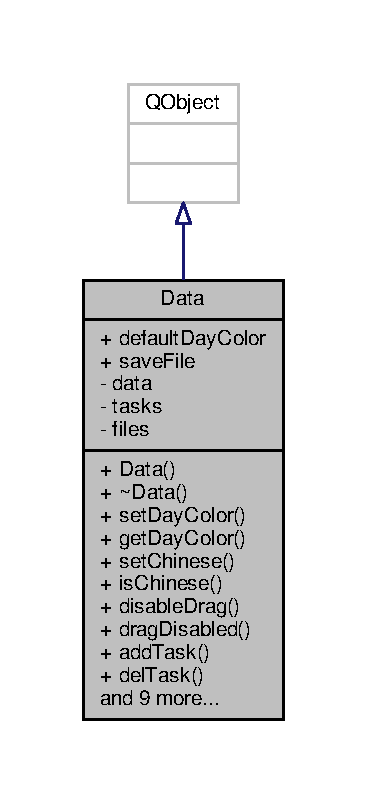
\includegraphics[width=176pt]{classData__inherit__graph}
\end{center}
\end{figure}


Collaboration diagram for Data\+:
\nopagebreak
\begin{figure}[H]
\begin{center}
\leavevmode
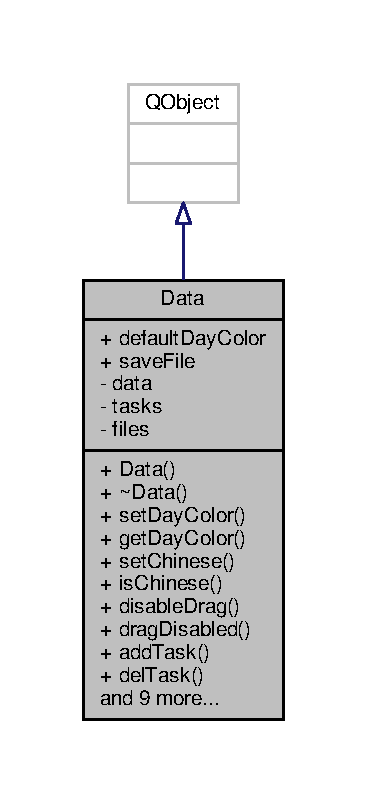
\includegraphics[width=176pt]{classData__coll__graph}
\end{center}
\end{figure}
\subsection*{Public Member Functions}
\begin{DoxyCompactItemize}
\item 
\hyperlink{classData_aaa7fad49e389b8fc445a6af43629609f}{Data} (Q\+Object $\ast$parent)
\begin{DoxyCompactList}\small\item\em Retrieve data from file. \end{DoxyCompactList}\item 
\hyperlink{classData_aab31956423290f0d62dcca47ab4d16dd}{$\sim$\+Data} ()
\begin{DoxyCompactList}\small\item\em Save data to file. \end{DoxyCompactList}\item 
void \hyperlink{classData_add1cb88caf02345f55126fd9ca934c3e}{set\+Day\+Color} (const Q\+Date \&day, const Q\+Color \&color)
\item 
Q\+Color \hyperlink{classData_a46470cbe33c14e9f24c8427e257a311e}{get\+Day\+Color} (const Q\+Date \&day) const 
\item 
void \hyperlink{classData_a051034d0bb71172fc8bbb3b395d2fe33}{set\+Chinese} (bool chinese)
\item 
bool \hyperlink{classData_ae538200aa5edaec5d01ee80bcda3f042}{is\+Chinese} () const 
\item 
void \hyperlink{classData_a8ece00071d9093892b80f1c994f99fb5}{disable\+Drag} (bool disable)
\item 
bool \hyperlink{classData_a5acaf7bb5f48c325240035351fe6b9bc}{drag\+Disabled} () const 
\item 
void \hyperlink{classData_a1a124e38871f90a177ddc34841c8e919}{add\+Task} (const Q\+Date \&day)
\begin{DoxyCompactList}\small\item\em Initialize a task for a day. \end{DoxyCompactList}\item 
void \hyperlink{classData_a16e96a143863d25e3dbcd875199e17f2}{del\+Task} (int index)
\begin{DoxyCompactList}\small\item\em Delete a task. \end{DoxyCompactList}\item 
Q\+List$<$ int $>$ \hyperlink{classData_aaf5830615d5abadbcb79f34dd89d4e0b}{find\+Task} (const Q\+Date \&day) const 
\begin{DoxyCompactList}\small\item\em Return indices of tasks for a day. \end{DoxyCompactList}\item 
const \hyperlink{classTask}{Task} $\ast$ \hyperlink{classData_ad46736016dc5ea00f2a98592e44e58f0}{task\+At} (int index) const 
\begin{DoxyCompactList}\small\item\em Get a task by index. \end{DoxyCompactList}\item 
\hyperlink{classTask}{Task} $\ast$ \hyperlink{classData_a4009575e5594138ae5b2d736480f46d2}{task\+At} (int index)
\item 
const Q\+List$<$ \hyperlink{classTask}{Task} $\ast$ $>$ \& \hyperlink{classData_a4e41f32520d3fc33a76d2e1eeda77883}{all\+Tasks} () const 
\begin{DoxyCompactList}\small\item\em Return all tasks. \end{DoxyCompactList}\item 
int \hyperlink{classData_aa571f90439e6d2890a94f86fc2324821}{add\+File} (const Q\+Date \&date, const Q\+Url \&path)
\begin{DoxyCompactList}\small\item\em Attach a file to a day. \end{DoxyCompactList}\item 
Q\+List$<$ \hyperlink{classFile}{File} $\ast$ $>$ \hyperlink{classData_af806515016b248a38ad33582509ffef5}{get\+File} (const Q\+Date \&date)
\item 
\hyperlink{classFile}{File} $\ast$ \hyperlink{classData_af5184411eed2650b9af48e21915c307f}{get\+File} (const Q\+Date \&date, int index)
\item 
void \hyperlink{classData_af027d735856b6505cf94ac3420700390}{del\+File} (const Q\+Date \&date, int index)
\item 
const Q\+Map$<$ Q\+Date, Q\+List$<$ \hyperlink{classFile}{File} $\ast$ $>$ $>$ \& \hyperlink{classData_a2a4f70a2e889f7f2a80a252571438030}{all\+Files} () const 
\begin{DoxyCompactList}\small\item\em return all files \end{DoxyCompactList}\end{DoxyCompactItemize}
\subsection*{Public Attributes}
\begin{DoxyCompactItemize}
\item 
const Q\+Color \hyperlink{classData_a5baa18f96bc11fe93566709af7fe16ba}{default\+Day\+Color} = Q\+Color(0x\+E0, 0x\+F\+F, 0x85, 0x\+D0)
\end{DoxyCompactItemize}
\subsection*{Static Public Attributes}
\begin{DoxyCompactItemize}
\item 
static constexpr const char $\ast$ \hyperlink{classData_a6781153c24e007e3540acf077fcbd2f7}{save\+File} = \char`\"{}savedcalendar.\+json\char`\"{}
\begin{DoxyCompactList}\small\item\em \hyperlink{classFile}{File} to save data. \end{DoxyCompactList}\end{DoxyCompactItemize}
\subsection*{Private Attributes}
\begin{DoxyCompactItemize}
\item 
Q\+Json\+Object \hyperlink{classData_ab6755adb48780d2aa2affe7497abe239}{data}
\item 
Q\+List$<$ \hyperlink{classTask}{Task} $\ast$ $>$ \hyperlink{classData_a532f7e91418f13e2f67dd3a47ff890f4}{tasks}
\item 
Q\+Map$<$ Q\+Date, Q\+List$<$ \hyperlink{classFile}{File} $\ast$ $>$ $>$ \hyperlink{classData_a5c3557bd928d1681876b174a5d7c3db9}{files}
\end{DoxyCompactItemize}


\subsection{Detailed Description}
Manage all user data and save it as J\+S\+ON format. 

\subsection{Constructor \& Destructor Documentation}
\index{Data@{Data}!Data@{Data}}
\index{Data@{Data}!Data@{Data}}
\subsubsection[{\texorpdfstring{Data(\+Q\+Object $\ast$parent)}{Data(QObject *parent)}}]{\setlength{\rightskip}{0pt plus 5cm}Data\+::\+Data (
\begin{DoxyParamCaption}
\item[{Q\+Object $\ast$}]{parent}
\end{DoxyParamCaption}
)\hspace{0.3cm}{\ttfamily [explicit]}}\hypertarget{classData_aaa7fad49e389b8fc445a6af43629609f}{}\label{classData_aaa7fad49e389b8fc445a6af43629609f}


Retrieve data from file. 

\index{Data@{Data}!````~Data@{$\sim$\+Data}}
\index{````~Data@{$\sim$\+Data}!Data@{Data}}
\subsubsection[{\texorpdfstring{$\sim$\+Data()}{~Data()}}]{\setlength{\rightskip}{0pt plus 5cm}Data\+::$\sim$\+Data (
\begin{DoxyParamCaption}
{}
\end{DoxyParamCaption}
)}\hypertarget{classData_aab31956423290f0d62dcca47ab4d16dd}{}\label{classData_aab31956423290f0d62dcca47ab4d16dd}


Save data to file. 



\subsection{Member Function Documentation}
\index{Data@{Data}!add\+File@{add\+File}}
\index{add\+File@{add\+File}!Data@{Data}}
\subsubsection[{\texorpdfstring{add\+File(const Q\+Date \&date, const Q\+Url \&path)}{addFile(const QDate &date, const QUrl &path)}}]{\setlength{\rightskip}{0pt plus 5cm}int Data\+::add\+File (
\begin{DoxyParamCaption}
\item[{const Q\+Date \&}]{date, }
\item[{const Q\+Url \&}]{path}
\end{DoxyParamCaption}
)}\hypertarget{classData_aa571f90439e6d2890a94f86fc2324821}{}\label{classData_aa571f90439e6d2890a94f86fc2324821}


Attach a file to a day. 

\begin{DoxyReturn}{Returns}
\+: index 
\end{DoxyReturn}
\index{Data@{Data}!add\+Task@{add\+Task}}
\index{add\+Task@{add\+Task}!Data@{Data}}
\subsubsection[{\texorpdfstring{add\+Task(const Q\+Date \&day)}{addTask(const QDate &day)}}]{\setlength{\rightskip}{0pt plus 5cm}void Data\+::add\+Task (
\begin{DoxyParamCaption}
\item[{const Q\+Date \&}]{day}
\end{DoxyParamCaption}
)}\hypertarget{classData_a1a124e38871f90a177ddc34841c8e919}{}\label{classData_a1a124e38871f90a177ddc34841c8e919}


Initialize a task for a day. 

\index{Data@{Data}!all\+Files@{all\+Files}}
\index{all\+Files@{all\+Files}!Data@{Data}}
\subsubsection[{\texorpdfstring{all\+Files() const }{allFiles() const }}]{\setlength{\rightskip}{0pt plus 5cm}const Q\+Map$<$ Q\+Date, Q\+List$<$ {\bf File} $\ast$ $>$ $>$ \& Data\+::all\+Files (
\begin{DoxyParamCaption}
{}
\end{DoxyParamCaption}
) const}\hypertarget{classData_a2a4f70a2e889f7f2a80a252571438030}{}\label{classData_a2a4f70a2e889f7f2a80a252571438030}


return all files 

\index{Data@{Data}!all\+Tasks@{all\+Tasks}}
\index{all\+Tasks@{all\+Tasks}!Data@{Data}}
\subsubsection[{\texorpdfstring{all\+Tasks() const }{allTasks() const }}]{\setlength{\rightskip}{0pt plus 5cm}const Q\+List$<$ {\bf Task} $\ast$ $>$ \& Data\+::all\+Tasks (
\begin{DoxyParamCaption}
{}
\end{DoxyParamCaption}
) const}\hypertarget{classData_a4e41f32520d3fc33a76d2e1eeda77883}{}\label{classData_a4e41f32520d3fc33a76d2e1eeda77883}


Return all tasks. 

\index{Data@{Data}!del\+File@{del\+File}}
\index{del\+File@{del\+File}!Data@{Data}}
\subsubsection[{\texorpdfstring{del\+File(const Q\+Date \&date, int index)}{delFile(const QDate &date, int index)}}]{\setlength{\rightskip}{0pt plus 5cm}void Data\+::del\+File (
\begin{DoxyParamCaption}
\item[{const Q\+Date \&}]{date, }
\item[{int}]{index}
\end{DoxyParamCaption}
)}\hypertarget{classData_af027d735856b6505cf94ac3420700390}{}\label{classData_af027d735856b6505cf94ac3420700390}
\index{Data@{Data}!del\+Task@{del\+Task}}
\index{del\+Task@{del\+Task}!Data@{Data}}
\subsubsection[{\texorpdfstring{del\+Task(int index)}{delTask(int index)}}]{\setlength{\rightskip}{0pt plus 5cm}void Data\+::del\+Task (
\begin{DoxyParamCaption}
\item[{int}]{index}
\end{DoxyParamCaption}
)}\hypertarget{classData_a16e96a143863d25e3dbcd875199e17f2}{}\label{classData_a16e96a143863d25e3dbcd875199e17f2}


Delete a task. 

\index{Data@{Data}!disable\+Drag@{disable\+Drag}}
\index{disable\+Drag@{disable\+Drag}!Data@{Data}}
\subsubsection[{\texorpdfstring{disable\+Drag(bool disable)}{disableDrag(bool disable)}}]{\setlength{\rightskip}{0pt plus 5cm}void Data\+::disable\+Drag (
\begin{DoxyParamCaption}
\item[{bool}]{disable}
\end{DoxyParamCaption}
)}\hypertarget{classData_a8ece00071d9093892b80f1c994f99fb5}{}\label{classData_a8ece00071d9093892b80f1c994f99fb5}
\index{Data@{Data}!drag\+Disabled@{drag\+Disabled}}
\index{drag\+Disabled@{drag\+Disabled}!Data@{Data}}
\subsubsection[{\texorpdfstring{drag\+Disabled() const }{dragDisabled() const }}]{\setlength{\rightskip}{0pt plus 5cm}bool Data\+::drag\+Disabled (
\begin{DoxyParamCaption}
{}
\end{DoxyParamCaption}
) const}\hypertarget{classData_a5acaf7bb5f48c325240035351fe6b9bc}{}\label{classData_a5acaf7bb5f48c325240035351fe6b9bc}
\index{Data@{Data}!find\+Task@{find\+Task}}
\index{find\+Task@{find\+Task}!Data@{Data}}
\subsubsection[{\texorpdfstring{find\+Task(const Q\+Date \&day) const }{findTask(const QDate &day) const }}]{\setlength{\rightskip}{0pt plus 5cm}Q\+List$<$ int $>$ Data\+::find\+Task (
\begin{DoxyParamCaption}
\item[{const Q\+Date \&}]{day}
\end{DoxyParamCaption}
) const}\hypertarget{classData_aaf5830615d5abadbcb79f34dd89d4e0b}{}\label{classData_aaf5830615d5abadbcb79f34dd89d4e0b}


Return indices of tasks for a day. 

\index{Data@{Data}!get\+Day\+Color@{get\+Day\+Color}}
\index{get\+Day\+Color@{get\+Day\+Color}!Data@{Data}}
\subsubsection[{\texorpdfstring{get\+Day\+Color(const Q\+Date \&day) const }{getDayColor(const QDate &day) const }}]{\setlength{\rightskip}{0pt plus 5cm}Q\+Color Data\+::get\+Day\+Color (
\begin{DoxyParamCaption}
\item[{const Q\+Date \&}]{day}
\end{DoxyParamCaption}
) const}\hypertarget{classData_a46470cbe33c14e9f24c8427e257a311e}{}\label{classData_a46470cbe33c14e9f24c8427e257a311e}
\index{Data@{Data}!get\+File@{get\+File}}
\index{get\+File@{get\+File}!Data@{Data}}
\subsubsection[{\texorpdfstring{get\+File(const Q\+Date \&date)}{getFile(const QDate &date)}}]{\setlength{\rightskip}{0pt plus 5cm}Q\+List$<$ {\bf File} $\ast$ $>$ Data\+::get\+File (
\begin{DoxyParamCaption}
\item[{const Q\+Date \&}]{date}
\end{DoxyParamCaption}
)}\hypertarget{classData_af806515016b248a38ad33582509ffef5}{}\label{classData_af806515016b248a38ad33582509ffef5}
\index{Data@{Data}!get\+File@{get\+File}}
\index{get\+File@{get\+File}!Data@{Data}}
\subsubsection[{\texorpdfstring{get\+File(const Q\+Date \&date, int index)}{getFile(const QDate &date, int index)}}]{\setlength{\rightskip}{0pt plus 5cm}{\bf File} $\ast$ Data\+::get\+File (
\begin{DoxyParamCaption}
\item[{const Q\+Date \&}]{date, }
\item[{int}]{index}
\end{DoxyParamCaption}
)}\hypertarget{classData_af5184411eed2650b9af48e21915c307f}{}\label{classData_af5184411eed2650b9af48e21915c307f}
\index{Data@{Data}!is\+Chinese@{is\+Chinese}}
\index{is\+Chinese@{is\+Chinese}!Data@{Data}}
\subsubsection[{\texorpdfstring{is\+Chinese() const }{isChinese() const }}]{\setlength{\rightskip}{0pt plus 5cm}bool Data\+::is\+Chinese (
\begin{DoxyParamCaption}
{}
\end{DoxyParamCaption}
) const}\hypertarget{classData_ae538200aa5edaec5d01ee80bcda3f042}{}\label{classData_ae538200aa5edaec5d01ee80bcda3f042}
\index{Data@{Data}!set\+Chinese@{set\+Chinese}}
\index{set\+Chinese@{set\+Chinese}!Data@{Data}}
\subsubsection[{\texorpdfstring{set\+Chinese(bool chinese)}{setChinese(bool chinese)}}]{\setlength{\rightskip}{0pt plus 5cm}void Data\+::set\+Chinese (
\begin{DoxyParamCaption}
\item[{bool}]{chinese}
\end{DoxyParamCaption}
)}\hypertarget{classData_a051034d0bb71172fc8bbb3b395d2fe33}{}\label{classData_a051034d0bb71172fc8bbb3b395d2fe33}
\index{Data@{Data}!set\+Day\+Color@{set\+Day\+Color}}
\index{set\+Day\+Color@{set\+Day\+Color}!Data@{Data}}
\subsubsection[{\texorpdfstring{set\+Day\+Color(const Q\+Date \&day, const Q\+Color \&color)}{setDayColor(const QDate &day, const QColor &color)}}]{\setlength{\rightskip}{0pt plus 5cm}void Data\+::set\+Day\+Color (
\begin{DoxyParamCaption}
\item[{const Q\+Date \&}]{day, }
\item[{const Q\+Color \&}]{color}
\end{DoxyParamCaption}
)}\hypertarget{classData_add1cb88caf02345f55126fd9ca934c3e}{}\label{classData_add1cb88caf02345f55126fd9ca934c3e}
\index{Data@{Data}!task\+At@{task\+At}}
\index{task\+At@{task\+At}!Data@{Data}}
\subsubsection[{\texorpdfstring{task\+At(int index) const }{taskAt(int index) const }}]{\setlength{\rightskip}{0pt plus 5cm}const {\bf Task} $\ast$ Data\+::task\+At (
\begin{DoxyParamCaption}
\item[{int}]{index}
\end{DoxyParamCaption}
) const}\hypertarget{classData_ad46736016dc5ea00f2a98592e44e58f0}{}\label{classData_ad46736016dc5ea00f2a98592e44e58f0}


Get a task by index. 

\index{Data@{Data}!task\+At@{task\+At}}
\index{task\+At@{task\+At}!Data@{Data}}
\subsubsection[{\texorpdfstring{task\+At(int index)}{taskAt(int index)}}]{\setlength{\rightskip}{0pt plus 5cm}{\bf Task} $\ast$ Data\+::task\+At (
\begin{DoxyParamCaption}
\item[{int}]{index}
\end{DoxyParamCaption}
)}\hypertarget{classData_a4009575e5594138ae5b2d736480f46d2}{}\label{classData_a4009575e5594138ae5b2d736480f46d2}


\subsection{Member Data Documentation}
\index{Data@{Data}!data@{data}}
\index{data@{data}!Data@{Data}}
\subsubsection[{\texorpdfstring{data}{data}}]{\setlength{\rightskip}{0pt plus 5cm}Q\+Json\+Object Data\+::data\hspace{0.3cm}{\ttfamily [private]}}\hypertarget{classData_ab6755adb48780d2aa2affe7497abe239}{}\label{classData_ab6755adb48780d2aa2affe7497abe239}
\index{Data@{Data}!default\+Day\+Color@{default\+Day\+Color}}
\index{default\+Day\+Color@{default\+Day\+Color}!Data@{Data}}
\subsubsection[{\texorpdfstring{default\+Day\+Color}{defaultDayColor}}]{\setlength{\rightskip}{0pt plus 5cm}const Q\+Color Data\+::default\+Day\+Color = Q\+Color(0x\+E0, 0x\+F\+F, 0x85, 0x\+D0)}\hypertarget{classData_a5baa18f96bc11fe93566709af7fe16ba}{}\label{classData_a5baa18f96bc11fe93566709af7fe16ba}
\index{Data@{Data}!files@{files}}
\index{files@{files}!Data@{Data}}
\subsubsection[{\texorpdfstring{files}{files}}]{\setlength{\rightskip}{0pt plus 5cm}Q\+Map$<$ Q\+Date, Q\+List$<${\bf File}$\ast$$>$ $>$ Data\+::files\hspace{0.3cm}{\ttfamily [private]}}\hypertarget{classData_a5c3557bd928d1681876b174a5d7c3db9}{}\label{classData_a5c3557bd928d1681876b174a5d7c3db9}
\index{Data@{Data}!save\+File@{save\+File}}
\index{save\+File@{save\+File}!Data@{Data}}
\subsubsection[{\texorpdfstring{save\+File}{saveFile}}]{\setlength{\rightskip}{0pt plus 5cm}constexpr const char$\ast$ Data\+::save\+File = \char`\"{}savedcalendar.\+json\char`\"{}\hspace{0.3cm}{\ttfamily [static]}}\hypertarget{classData_a6781153c24e007e3540acf077fcbd2f7}{}\label{classData_a6781153c24e007e3540acf077fcbd2f7}


\hyperlink{classFile}{File} to save data. 

\index{Data@{Data}!tasks@{tasks}}
\index{tasks@{tasks}!Data@{Data}}
\subsubsection[{\texorpdfstring{tasks}{tasks}}]{\setlength{\rightskip}{0pt plus 5cm}Q\+List$<${\bf Task}$\ast$$>$ Data\+::tasks\hspace{0.3cm}{\ttfamily [private]}}\hypertarget{classData_a532f7e91418f13e2f67dd3a47ff890f4}{}\label{classData_a532f7e91418f13e2f67dd3a47ff890f4}


The documentation for this class was generated from the following files\+:\begin{DoxyCompactItemize}
\item 
\hyperlink{data_8h}{data.\+h}\item 
\hyperlink{data_8cpp}{data.\+cpp}\end{DoxyCompactItemize}

\hypertarget{classDragData}{}\section{Drag\+Data Class Reference}
\label{classDragData}\index{Drag\+Data@{Drag\+Data}}


Create a file and return its url when requested.  




{\ttfamily \#include $<$dragdata.\+h$>$}



Inheritance diagram for Drag\+Data\+:
\nopagebreak
\begin{figure}[H]
\begin{center}
\leavevmode
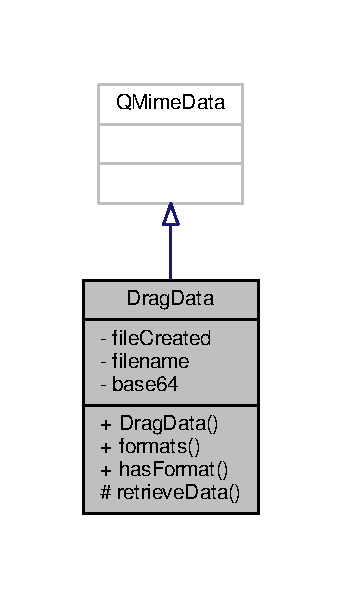
\includegraphics[width=164pt]{classDragData__inherit__graph}
\end{center}
\end{figure}


Collaboration diagram for Drag\+Data\+:
\nopagebreak
\begin{figure}[H]
\begin{center}
\leavevmode
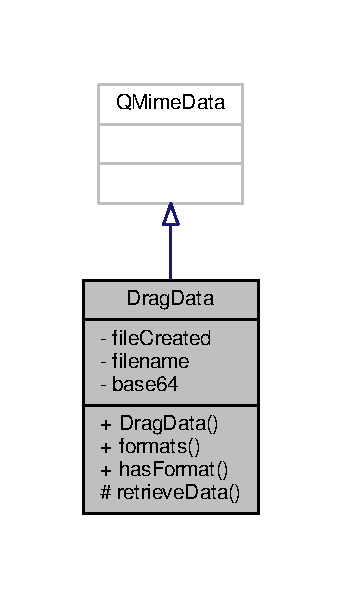
\includegraphics[width=164pt]{classDragData__coll__graph}
\end{center}
\end{figure}
\subsection*{Public Member Functions}
\begin{DoxyCompactItemize}
\item 
\hyperlink{classDragData_a09c41f96b24d51674b88d17168b33d78}{Drag\+Data} (const Q\+String \&\+\_\+filename, const Q\+String \+\_\+base64)
\item 
Q\+String\+List \hyperlink{classDragData_ae8564afb0c0f5fb2868c39d9a922974e}{formats} () const override
\item 
bool \hyperlink{classDragData_a02f40827e954229013d893ec7c148a96}{has\+Format} (const Q\+String \&mime\+Type) const override
\end{DoxyCompactItemize}
\subsection*{Protected Member Functions}
\begin{DoxyCompactItemize}
\item 
Q\+Variant \hyperlink{classDragData_abb3bb5ffb7ac287fe5c14d5d5a29831d}{retrieve\+Data} (const Q\+String \&mimetype, Q\+Variant\+::\+Type preferred\+Type) const override
\end{DoxyCompactItemize}
\subsection*{Private Attributes}
\begin{DoxyCompactItemize}
\item 
bool \hyperlink{classDragData_a2037ac6c96051425bc5c810f560ebc96}{file\+Created}
\begin{DoxyCompactList}\small\item\em Only create temporary file once. \end{DoxyCompactList}\item 
Q\+String \hyperlink{classDragData_a3ec29e3d1a3a05e44582a724244256f5}{filename}
\item 
Q\+String \hyperlink{classDragData_a96f7b850cb7dfed17dc74057340384e3}{base64}
\begin{DoxyCompactList}\small\item\em file content in Base64 \end{DoxyCompactList}\end{DoxyCompactItemize}


\subsection{Detailed Description}
Create a file and return its url when requested. 

\subsection{Constructor \& Destructor Documentation}
\index{Drag\+Data@{Drag\+Data}!Drag\+Data@{Drag\+Data}}
\index{Drag\+Data@{Drag\+Data}!Drag\+Data@{Drag\+Data}}
\subsubsection[{\texorpdfstring{Drag\+Data(const Q\+String \&\+\_\+filename, const Q\+String \+\_\+base64)}{DragData(const QString &_filename, const QString _base64)}}]{\setlength{\rightskip}{0pt plus 5cm}Drag\+Data\+::\+Drag\+Data (
\begin{DoxyParamCaption}
\item[{const Q\+String \&}]{\+\_\+filename, }
\item[{const Q\+String}]{\+\_\+base64}
\end{DoxyParamCaption}
)}\hypertarget{classDragData_a09c41f96b24d51674b88d17168b33d78}{}\label{classDragData_a09c41f96b24d51674b88d17168b33d78}


\subsection{Member Function Documentation}
\index{Drag\+Data@{Drag\+Data}!formats@{formats}}
\index{formats@{formats}!Drag\+Data@{Drag\+Data}}
\subsubsection[{\texorpdfstring{formats() const override}{formats() const override}}]{\setlength{\rightskip}{0pt plus 5cm}Q\+String\+List Drag\+Data\+::formats (
\begin{DoxyParamCaption}
{}
\end{DoxyParamCaption}
) const\hspace{0.3cm}{\ttfamily [override]}}\hypertarget{classDragData_ae8564afb0c0f5fb2868c39d9a922974e}{}\label{classDragData_ae8564afb0c0f5fb2868c39d9a922974e}
\index{Drag\+Data@{Drag\+Data}!has\+Format@{has\+Format}}
\index{has\+Format@{has\+Format}!Drag\+Data@{Drag\+Data}}
\subsubsection[{\texorpdfstring{has\+Format(const Q\+String \&mime\+Type) const override}{hasFormat(const QString &mimeType) const override}}]{\setlength{\rightskip}{0pt plus 5cm}bool Drag\+Data\+::has\+Format (
\begin{DoxyParamCaption}
\item[{const Q\+String \&}]{mime\+Type}
\end{DoxyParamCaption}
) const\hspace{0.3cm}{\ttfamily [override]}}\hypertarget{classDragData_a02f40827e954229013d893ec7c148a96}{}\label{classDragData_a02f40827e954229013d893ec7c148a96}
\index{Drag\+Data@{Drag\+Data}!retrieve\+Data@{retrieve\+Data}}
\index{retrieve\+Data@{retrieve\+Data}!Drag\+Data@{Drag\+Data}}
\subsubsection[{\texorpdfstring{retrieve\+Data(const Q\+String \&mimetype, Q\+Variant\+::\+Type preferred\+Type) const override}{retrieveData(const QString &mimetype, QVariant::Type preferredType) const override}}]{\setlength{\rightskip}{0pt plus 5cm}Q\+Variant Drag\+Data\+::retrieve\+Data (
\begin{DoxyParamCaption}
\item[{const Q\+String \&}]{mimetype, }
\item[{Q\+Variant\+::\+Type}]{preferred\+Type}
\end{DoxyParamCaption}
) const\hspace{0.3cm}{\ttfamily [override]}, {\ttfamily [protected]}}\hypertarget{classDragData_abb3bb5ffb7ac287fe5c14d5d5a29831d}{}\label{classDragData_abb3bb5ffb7ac287fe5c14d5d5a29831d}


\subsection{Member Data Documentation}
\index{Drag\+Data@{Drag\+Data}!base64@{base64}}
\index{base64@{base64}!Drag\+Data@{Drag\+Data}}
\subsubsection[{\texorpdfstring{base64}{base64}}]{\setlength{\rightskip}{0pt plus 5cm}Q\+String Drag\+Data\+::base64\hspace{0.3cm}{\ttfamily [private]}}\hypertarget{classDragData_a96f7b850cb7dfed17dc74057340384e3}{}\label{classDragData_a96f7b850cb7dfed17dc74057340384e3}


file content in Base64 

\index{Drag\+Data@{Drag\+Data}!file\+Created@{file\+Created}}
\index{file\+Created@{file\+Created}!Drag\+Data@{Drag\+Data}}
\subsubsection[{\texorpdfstring{file\+Created}{fileCreated}}]{\setlength{\rightskip}{0pt plus 5cm}bool Drag\+Data\+::file\+Created\hspace{0.3cm}{\ttfamily [mutable]}, {\ttfamily [private]}}\hypertarget{classDragData_a2037ac6c96051425bc5c810f560ebc96}{}\label{classDragData_a2037ac6c96051425bc5c810f560ebc96}


Only create temporary file once. 

\index{Drag\+Data@{Drag\+Data}!filename@{filename}}
\index{filename@{filename}!Drag\+Data@{Drag\+Data}}
\subsubsection[{\texorpdfstring{filename}{filename}}]{\setlength{\rightskip}{0pt plus 5cm}Q\+String Drag\+Data\+::filename\hspace{0.3cm}{\ttfamily [private]}}\hypertarget{classDragData_a3ec29e3d1a3a05e44582a724244256f5}{}\label{classDragData_a3ec29e3d1a3a05e44582a724244256f5}


The documentation for this class was generated from the following files\+:\begin{DoxyCompactItemize}
\item 
\hyperlink{dragdata_8h}{dragdata.\+h}\item 
\hyperlink{dragdata_8cpp}{dragdata.\+cpp}\end{DoxyCompactItemize}

\hypertarget{classFile}{}\section{File Class Reference}
\label{classFile}\index{File@{File}}


A file dragged in by user. Encode its content in Base64.  




{\ttfamily \#include $<$file.\+h$>$}



Inheritance diagram for File\+:
\nopagebreak
\begin{figure}[H]
\begin{center}
\leavevmode
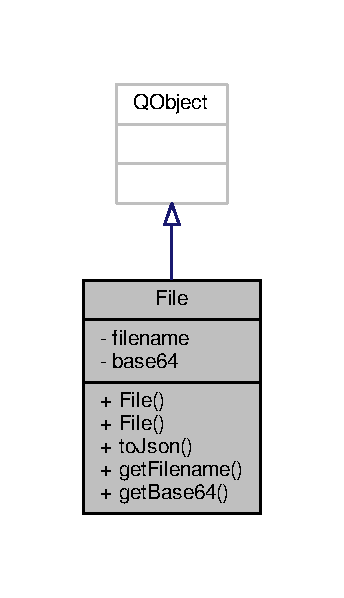
\includegraphics[width=165pt]{classFile__inherit__graph}
\end{center}
\end{figure}


Collaboration diagram for File\+:
\nopagebreak
\begin{figure}[H]
\begin{center}
\leavevmode
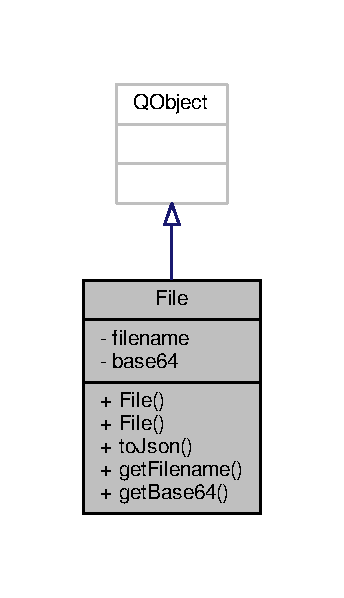
\includegraphics[width=165pt]{classFile__coll__graph}
\end{center}
\end{figure}
\subsection*{Public Member Functions}
\begin{DoxyCompactItemize}
\item 
\hyperlink{classFile_af0347154cd72c6e3d7081c5d6be094b6}{File} (Q\+Json\+Value\+Ref json, Q\+Object $\ast$parent)
\item 
\hyperlink{classFile_aae009478998b830041fef4a1fb5157a9}{File} (const Q\+Url \&path, Q\+Object $\ast$parent)
\item 
Q\+Json\+Value \hyperlink{classFile_a8bae9c09c895961d8a51fc31b92877ec}{to\+Json} () const 
\item 
const Q\+String \& \hyperlink{classFile_aa870c4efb7add8f3617309a21adc728a}{get\+Filename} () const 
\item 
const Q\+String \& \hyperlink{classFile_afb5e504133cc25beed457a52b6c28a8d}{get\+Base64} () const 
\end{DoxyCompactItemize}
\subsection*{Private Attributes}
\begin{DoxyCompactItemize}
\item 
Q\+String \hyperlink{classFile_aa57d3c49fb1dd72a1df15c1033a9c0a4}{filename}
\item 
Q\+String \hyperlink{classFile_a84fadb8b406869284dc6fd09c9de36a2}{base64}
\end{DoxyCompactItemize}


\subsection{Detailed Description}
A file dragged in by user. Encode its content in Base64. 

\subsection{Constructor \& Destructor Documentation}
\index{File@{File}!File@{File}}
\index{File@{File}!File@{File}}
\subsubsection[{\texorpdfstring{File(\+Q\+Json\+Value\+Ref json, Q\+Object $\ast$parent)}{File(QJsonValueRef json, QObject *parent)}}]{\setlength{\rightskip}{0pt plus 5cm}File\+::\+File (
\begin{DoxyParamCaption}
\item[{Q\+Json\+Value\+Ref}]{json, }
\item[{Q\+Object $\ast$}]{parent}
\end{DoxyParamCaption}
)\hspace{0.3cm}{\ttfamily [explicit]}}\hypertarget{classFile_af0347154cd72c6e3d7081c5d6be094b6}{}\label{classFile_af0347154cd72c6e3d7081c5d6be094b6}
\index{File@{File}!File@{File}}
\index{File@{File}!File@{File}}
\subsubsection[{\texorpdfstring{File(const Q\+Url \&path, Q\+Object $\ast$parent)}{File(const QUrl &path, QObject *parent)}}]{\setlength{\rightskip}{0pt plus 5cm}File\+::\+File (
\begin{DoxyParamCaption}
\item[{const Q\+Url \&}]{path, }
\item[{Q\+Object $\ast$}]{parent}
\end{DoxyParamCaption}
)\hspace{0.3cm}{\ttfamily [explicit]}}\hypertarget{classFile_aae009478998b830041fef4a1fb5157a9}{}\label{classFile_aae009478998b830041fef4a1fb5157a9}


\subsection{Member Function Documentation}
\index{File@{File}!get\+Base64@{get\+Base64}}
\index{get\+Base64@{get\+Base64}!File@{File}}
\subsubsection[{\texorpdfstring{get\+Base64() const }{getBase64() const }}]{\setlength{\rightskip}{0pt plus 5cm}const Q\+String \& File\+::get\+Base64 (
\begin{DoxyParamCaption}
{}
\end{DoxyParamCaption}
) const}\hypertarget{classFile_afb5e504133cc25beed457a52b6c28a8d}{}\label{classFile_afb5e504133cc25beed457a52b6c28a8d}
\index{File@{File}!get\+Filename@{get\+Filename}}
\index{get\+Filename@{get\+Filename}!File@{File}}
\subsubsection[{\texorpdfstring{get\+Filename() const }{getFilename() const }}]{\setlength{\rightskip}{0pt plus 5cm}const Q\+String \& File\+::get\+Filename (
\begin{DoxyParamCaption}
{}
\end{DoxyParamCaption}
) const}\hypertarget{classFile_aa870c4efb7add8f3617309a21adc728a}{}\label{classFile_aa870c4efb7add8f3617309a21adc728a}
\index{File@{File}!to\+Json@{to\+Json}}
\index{to\+Json@{to\+Json}!File@{File}}
\subsubsection[{\texorpdfstring{to\+Json() const }{toJson() const }}]{\setlength{\rightskip}{0pt plus 5cm}Q\+Json\+Value File\+::to\+Json (
\begin{DoxyParamCaption}
{}
\end{DoxyParamCaption}
) const}\hypertarget{classFile_a8bae9c09c895961d8a51fc31b92877ec}{}\label{classFile_a8bae9c09c895961d8a51fc31b92877ec}


\subsection{Member Data Documentation}
\index{File@{File}!base64@{base64}}
\index{base64@{base64}!File@{File}}
\subsubsection[{\texorpdfstring{base64}{base64}}]{\setlength{\rightskip}{0pt plus 5cm}Q\+String File\+::base64\hspace{0.3cm}{\ttfamily [private]}}\hypertarget{classFile_a84fadb8b406869284dc6fd09c9de36a2}{}\label{classFile_a84fadb8b406869284dc6fd09c9de36a2}
\index{File@{File}!filename@{filename}}
\index{filename@{filename}!File@{File}}
\subsubsection[{\texorpdfstring{filename}{filename}}]{\setlength{\rightskip}{0pt plus 5cm}Q\+String File\+::filename\hspace{0.3cm}{\ttfamily [private]}}\hypertarget{classFile_aa57d3c49fb1dd72a1df15c1033a9c0a4}{}\label{classFile_aa57d3c49fb1dd72a1df15c1033a9c0a4}


The documentation for this class was generated from the following files\+:\begin{DoxyCompactItemize}
\item 
\hyperlink{file_8h}{file.\+h}\item 
\hyperlink{file_8cpp}{file.\+cpp}\end{DoxyCompactItemize}

\hypertarget{classFileDisplay}{}\section{File\+Display Class Reference}
\label{classFileDisplay}\index{File\+Display@{File\+Display}}


Display a file dragged in by user.  




{\ttfamily \#include $<$filedisplay.\+h$>$}



Inheritance diagram for File\+Display\+:
\nopagebreak
\begin{figure}[H]
\begin{center}
\leavevmode
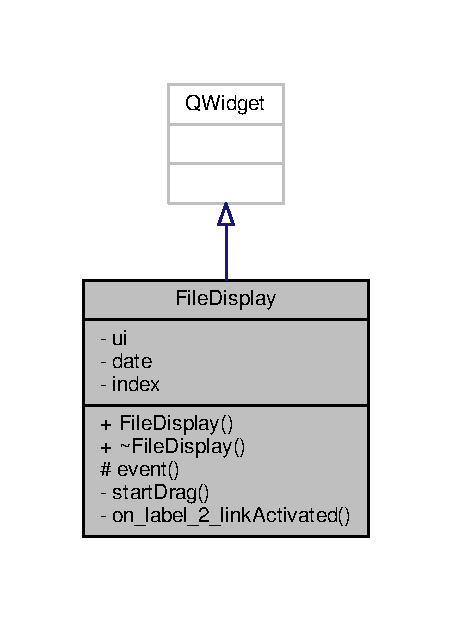
\includegraphics[width=217pt]{classFileDisplay__inherit__graph}
\end{center}
\end{figure}


Collaboration diagram for File\+Display\+:
\nopagebreak
\begin{figure}[H]
\begin{center}
\leavevmode
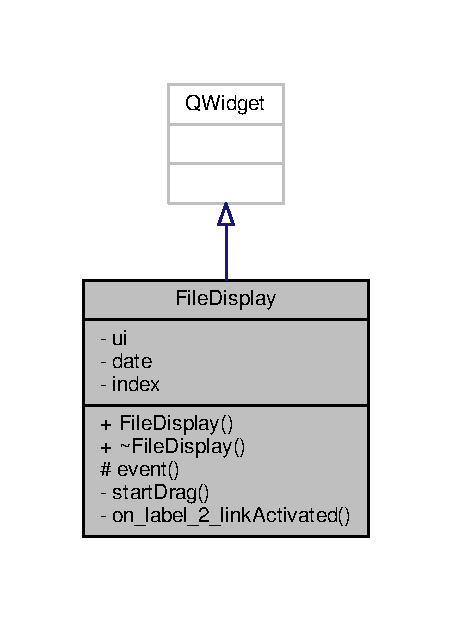
\includegraphics[width=217pt]{classFileDisplay__coll__graph}
\end{center}
\end{figure}
\subsection*{Signals}
\begin{DoxyCompactItemize}
\item 
void \hyperlink{classFileDisplay_a82b770665aa3e87b8945871e65124c16}{require\+Refresh} ()
\end{DoxyCompactItemize}
\subsection*{Public Member Functions}
\begin{DoxyCompactItemize}
\item 
\hyperlink{classFileDisplay_a78758d0d7cf80cbe6f6a400cc9bb2bcd}{File\+Display} (const Q\+Date \&\+\_\+date, int \+\_\+index, Q\+Widget $\ast$parent)
\item 
\hyperlink{classFileDisplay_a57b1b3b135ad210a87ff04c7652dd846}{$\sim$\+File\+Display} ()
\end{DoxyCompactItemize}
\subsection*{Protected Member Functions}
\begin{DoxyCompactItemize}
\item 
bool \hyperlink{classFileDisplay_a679e676c4496c0b441753c5e6670be81}{event} (Q\+Event $\ast$event) override
\end{DoxyCompactItemize}
\subsection*{Private Slots}
\begin{DoxyCompactItemize}
\item 
void \hyperlink{classFileDisplay_aaffa2b93339b7a84b8af28847fa1f099}{start\+Drag} ()
\item 
void \hyperlink{classFileDisplay_a62f53655eacd44d1026f7fe7808e7a1f}{on\+\_\+label\+\_\+2\+\_\+link\+Activated} (const Q\+String \&link)
\end{DoxyCompactItemize}
\subsection*{Private Attributes}
\begin{DoxyCompactItemize}
\item 
Ui\+::\+File\+Display $\ast$ \hyperlink{classFileDisplay_a0f69fef4d0c94b979e55dd8d97f196c7}{ui}
\item 
Q\+Date \hyperlink{classFileDisplay_a0a82f6e8e67ad36ef80575ec6be86372}{date}
\item 
int \hyperlink{classFileDisplay_aceb0af801357d0fff3b09bd1285136f7}{index}
\end{DoxyCompactItemize}


\subsection{Detailed Description}
Display a file dragged in by user. 

\subsection{Constructor \& Destructor Documentation}
\index{File\+Display@{File\+Display}!File\+Display@{File\+Display}}
\index{File\+Display@{File\+Display}!File\+Display@{File\+Display}}
\subsubsection[{\texorpdfstring{File\+Display(const Q\+Date \&\+\_\+date, int \+\_\+index, Q\+Widget $\ast$parent)}{FileDisplay(const QDate &_date, int _index, QWidget *parent)}}]{\setlength{\rightskip}{0pt plus 5cm}File\+Display\+::\+File\+Display (
\begin{DoxyParamCaption}
\item[{const Q\+Date \&}]{\+\_\+date, }
\item[{int}]{\+\_\+index, }
\item[{Q\+Widget $\ast$}]{parent}
\end{DoxyParamCaption}
)\hspace{0.3cm}{\ttfamily [explicit]}}\hypertarget{classFileDisplay_a78758d0d7cf80cbe6f6a400cc9bb2bcd}{}\label{classFileDisplay_a78758d0d7cf80cbe6f6a400cc9bb2bcd}
\index{File\+Display@{File\+Display}!````~File\+Display@{$\sim$\+File\+Display}}
\index{````~File\+Display@{$\sim$\+File\+Display}!File\+Display@{File\+Display}}
\subsubsection[{\texorpdfstring{$\sim$\+File\+Display()}{~FileDisplay()}}]{\setlength{\rightskip}{0pt plus 5cm}File\+Display\+::$\sim$\+File\+Display (
\begin{DoxyParamCaption}
{}
\end{DoxyParamCaption}
)}\hypertarget{classFileDisplay_a57b1b3b135ad210a87ff04c7652dd846}{}\label{classFileDisplay_a57b1b3b135ad210a87ff04c7652dd846}


\subsection{Member Function Documentation}
\index{File\+Display@{File\+Display}!event@{event}}
\index{event@{event}!File\+Display@{File\+Display}}
\subsubsection[{\texorpdfstring{event(\+Q\+Event $\ast$event) override}{event(QEvent *event) override}}]{\setlength{\rightskip}{0pt plus 5cm}bool File\+Display\+::event (
\begin{DoxyParamCaption}
\item[{Q\+Event $\ast$}]{event}
\end{DoxyParamCaption}
)\hspace{0.3cm}{\ttfamily [override]}, {\ttfamily [protected]}}\hypertarget{classFileDisplay_a679e676c4496c0b441753c5e6670be81}{}\label{classFileDisplay_a679e676c4496c0b441753c5e6670be81}
\index{File\+Display@{File\+Display}!on\+\_\+label\+\_\+2\+\_\+link\+Activated@{on\+\_\+label\+\_\+2\+\_\+link\+Activated}}
\index{on\+\_\+label\+\_\+2\+\_\+link\+Activated@{on\+\_\+label\+\_\+2\+\_\+link\+Activated}!File\+Display@{File\+Display}}
\subsubsection[{\texorpdfstring{on\+\_\+label\+\_\+2\+\_\+link\+Activated}{on_label_2_linkActivated}}]{\setlength{\rightskip}{0pt plus 5cm}void File\+Display\+::on\+\_\+label\+\_\+2\+\_\+link\+Activated (
\begin{DoxyParamCaption}
\item[{const Q\+String \&}]{link}
\end{DoxyParamCaption}
)\hspace{0.3cm}{\ttfamily [private]}, {\ttfamily [slot]}}\hypertarget{classFileDisplay_a62f53655eacd44d1026f7fe7808e7a1f}{}\label{classFileDisplay_a62f53655eacd44d1026f7fe7808e7a1f}
\index{File\+Display@{File\+Display}!require\+Refresh@{require\+Refresh}}
\index{require\+Refresh@{require\+Refresh}!File\+Display@{File\+Display}}
\subsubsection[{\texorpdfstring{require\+Refresh}{requireRefresh}}]{\setlength{\rightskip}{0pt plus 5cm}void File\+Display\+::require\+Refresh (
\begin{DoxyParamCaption}
{}
\end{DoxyParamCaption}
)\hspace{0.3cm}{\ttfamily [signal]}}\hypertarget{classFileDisplay_a82b770665aa3e87b8945871e65124c16}{}\label{classFileDisplay_a82b770665aa3e87b8945871e65124c16}
\index{File\+Display@{File\+Display}!start\+Drag@{start\+Drag}}
\index{start\+Drag@{start\+Drag}!File\+Display@{File\+Display}}
\subsubsection[{\texorpdfstring{start\+Drag}{startDrag}}]{\setlength{\rightskip}{0pt plus 5cm}void File\+Display\+::start\+Drag (
\begin{DoxyParamCaption}
{}
\end{DoxyParamCaption}
)\hspace{0.3cm}{\ttfamily [private]}, {\ttfamily [slot]}}\hypertarget{classFileDisplay_aaffa2b93339b7a84b8af28847fa1f099}{}\label{classFileDisplay_aaffa2b93339b7a84b8af28847fa1f099}


\subsection{Member Data Documentation}
\index{File\+Display@{File\+Display}!date@{date}}
\index{date@{date}!File\+Display@{File\+Display}}
\subsubsection[{\texorpdfstring{date}{date}}]{\setlength{\rightskip}{0pt plus 5cm}Q\+Date File\+Display\+::date\hspace{0.3cm}{\ttfamily [private]}}\hypertarget{classFileDisplay_a0a82f6e8e67ad36ef80575ec6be86372}{}\label{classFileDisplay_a0a82f6e8e67ad36ef80575ec6be86372}
\index{File\+Display@{File\+Display}!index@{index}}
\index{index@{index}!File\+Display@{File\+Display}}
\subsubsection[{\texorpdfstring{index}{index}}]{\setlength{\rightskip}{0pt plus 5cm}int File\+Display\+::index\hspace{0.3cm}{\ttfamily [private]}}\hypertarget{classFileDisplay_aceb0af801357d0fff3b09bd1285136f7}{}\label{classFileDisplay_aceb0af801357d0fff3b09bd1285136f7}
\index{File\+Display@{File\+Display}!ui@{ui}}
\index{ui@{ui}!File\+Display@{File\+Display}}
\subsubsection[{\texorpdfstring{ui}{ui}}]{\setlength{\rightskip}{0pt plus 5cm}Ui\+::\+File\+Display$\ast$ File\+Display\+::ui\hspace{0.3cm}{\ttfamily [private]}}\hypertarget{classFileDisplay_a0f69fef4d0c94b979e55dd8d97f196c7}{}\label{classFileDisplay_a0f69fef4d0c94b979e55dd8d97f196c7}


The documentation for this class was generated from the following files\+:\begin{DoxyCompactItemize}
\item 
\hyperlink{filedisplay_8h}{filedisplay.\+h}\item 
\hyperlink{filedisplay_8cpp}{filedisplay.\+cpp}\end{DoxyCompactItemize}

\hypertarget{classHelp}{}\section{Help Class Reference}
\label{classHelp}\index{Help@{Help}}


{\ttfamily \#include $<$help.\+h$>$}



Inheritance diagram for Help\+:
\nopagebreak
\begin{figure}[H]
\begin{center}
\leavevmode
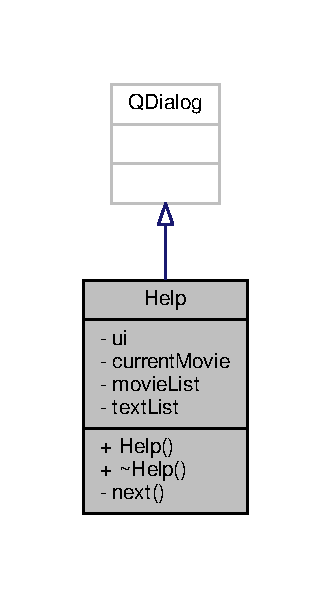
\includegraphics[width=159pt]{classHelp__inherit__graph}
\end{center}
\end{figure}


Collaboration diagram for Help\+:
\nopagebreak
\begin{figure}[H]
\begin{center}
\leavevmode
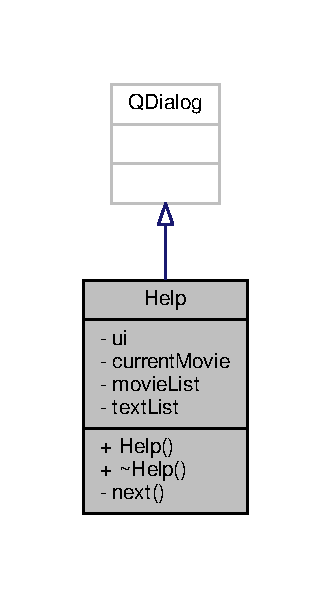
\includegraphics[width=159pt]{classHelp__coll__graph}
\end{center}
\end{figure}
\subsection*{Public Member Functions}
\begin{DoxyCompactItemize}
\item 
\hyperlink{classHelp_a7359f816eb2dab34e4c7017e36c9654d}{Help} (Q\+Widget $\ast$parent=0)
\item 
\hyperlink{classHelp_a123b4195136758782058cb78cbd0baf7}{$\sim$\+Help} ()
\end{DoxyCompactItemize}
\subsection*{Private Slots}
\begin{DoxyCompactItemize}
\item 
void \hyperlink{classHelp_a22bf8a30b57727d051b07e81cbcf08af}{next} ()
\end{DoxyCompactItemize}
\subsection*{Private Attributes}
\begin{DoxyCompactItemize}
\item 
Ui\+::\+Help $\ast$ \hyperlink{classHelp_a2b64cd3a7d7dc1e6d44c575d4df6dc0d}{ui}
\item 
int \hyperlink{classHelp_a0c024355540423400020e10b1b59f8b6}{current\+Movie}
\item 
const Q\+List$<$ Q\+Movie $\ast$ $>$ \hyperlink{classHelp_add4de4d4640b971e5e80fac57f027099}{movie\+List}
\item 
const Q\+List$<$ Q\+String $>$ \hyperlink{classHelp_a0c53a50be73195a84b7828ff0f576430}{text\+List}
\end{DoxyCompactItemize}


\subsection{Constructor \& Destructor Documentation}
\index{Help@{Help}!Help@{Help}}
\index{Help@{Help}!Help@{Help}}
\subsubsection[{\texorpdfstring{Help(\+Q\+Widget $\ast$parent=0)}{Help(QWidget *parent=0)}}]{\setlength{\rightskip}{0pt plus 5cm}Help\+::\+Help (
\begin{DoxyParamCaption}
\item[{Q\+Widget $\ast$}]{parent = {\ttfamily 0}}
\end{DoxyParamCaption}
)\hspace{0.3cm}{\ttfamily [explicit]}}\hypertarget{classHelp_a7359f816eb2dab34e4c7017e36c9654d}{}\label{classHelp_a7359f816eb2dab34e4c7017e36c9654d}
\index{Help@{Help}!````~Help@{$\sim$\+Help}}
\index{````~Help@{$\sim$\+Help}!Help@{Help}}
\subsubsection[{\texorpdfstring{$\sim$\+Help()}{~Help()}}]{\setlength{\rightskip}{0pt plus 5cm}Help\+::$\sim$\+Help (
\begin{DoxyParamCaption}
{}
\end{DoxyParamCaption}
)}\hypertarget{classHelp_a123b4195136758782058cb78cbd0baf7}{}\label{classHelp_a123b4195136758782058cb78cbd0baf7}


\subsection{Member Function Documentation}
\index{Help@{Help}!next@{next}}
\index{next@{next}!Help@{Help}}
\subsubsection[{\texorpdfstring{next}{next}}]{\setlength{\rightskip}{0pt plus 5cm}void Help\+::next (
\begin{DoxyParamCaption}
{}
\end{DoxyParamCaption}
)\hspace{0.3cm}{\ttfamily [private]}, {\ttfamily [slot]}}\hypertarget{classHelp_a22bf8a30b57727d051b07e81cbcf08af}{}\label{classHelp_a22bf8a30b57727d051b07e81cbcf08af}


\subsection{Member Data Documentation}
\index{Help@{Help}!current\+Movie@{current\+Movie}}
\index{current\+Movie@{current\+Movie}!Help@{Help}}
\subsubsection[{\texorpdfstring{current\+Movie}{currentMovie}}]{\setlength{\rightskip}{0pt plus 5cm}int Help\+::current\+Movie\hspace{0.3cm}{\ttfamily [private]}}\hypertarget{classHelp_a0c024355540423400020e10b1b59f8b6}{}\label{classHelp_a0c024355540423400020e10b1b59f8b6}
\index{Help@{Help}!movie\+List@{movie\+List}}
\index{movie\+List@{movie\+List}!Help@{Help}}
\subsubsection[{\texorpdfstring{movie\+List}{movieList}}]{\setlength{\rightskip}{0pt plus 5cm}const Q\+List$<$Q\+Movie$\ast$$>$ Help\+::movie\+List\hspace{0.3cm}{\ttfamily [private]}}\hypertarget{classHelp_add4de4d4640b971e5e80fac57f027099}{}\label{classHelp_add4de4d4640b971e5e80fac57f027099}
{\bfseries Initial value\+:}
\begin{DoxyCode}
= \{
        \textcolor{keyword}{new} QMovie(\textcolor{stringliteral}{":/video/change-color.gif"}, \textcolor{stringliteral}{"GIF"}, \textcolor{keyword}{this}),
        \textcolor{keyword}{new} QMovie(\textcolor{stringliteral}{":/video/add-task.gif"}, \textcolor{stringliteral}{"GIF"}, \textcolor{keyword}{this}),
        \textcolor{keyword}{new} QMovie(\textcolor{stringliteral}{":/video/del-task.gif"}, \textcolor{stringliteral}{"GIF"}, \textcolor{keyword}{this}),
        \textcolor{keyword}{new} QMovie(\textcolor{stringliteral}{":/video/drag-files.gif"}, \textcolor{stringliteral}{"GIF"}, \textcolor{keyword}{this}),
        \textcolor{keyword}{new} QMovie(\textcolor{stringliteral}{":/video/export-import.gif"}, \textcolor{stringliteral}{"GIF"}, \textcolor{keyword}{this}),
        \textcolor{keyword}{new} QMovie(\textcolor{stringliteral}{":/video/pin.gif"}, \textcolor{stringliteral}{"GIF"}, \textcolor{keyword}{this}),
        \textcolor{keyword}{new} QMovie(\textcolor{stringliteral}{":/video/mode.gif"}, \textcolor{stringliteral}{"GIF"}, \textcolor{keyword}{this})
    \}
\end{DoxyCode}
\index{Help@{Help}!text\+List@{text\+List}}
\index{text\+List@{text\+List}!Help@{Help}}
\subsubsection[{\texorpdfstring{text\+List}{textList}}]{\setlength{\rightskip}{0pt plus 5cm}const Q\+List$<$Q\+String$>$ Help\+::text\+List\hspace{0.3cm}{\ttfamily [private]}}\hypertarget{classHelp_a0c53a50be73195a84b7828ff0f576430}{}\label{classHelp_a0c53a50be73195a84b7828ff0f576430}
{\bfseries Initial value\+:}
\begin{DoxyCode}
= \{
        tr(\textcolor{stringliteral}{"Double-click on a day to set its color."}),
        tr(\textcolor{stringliteral}{"Add a task and set it as repeated optionally."}),
        tr(\textcolor{stringliteral}{"Delete a task just for a day or delete all repeated tasks."}),
        tr(\textcolor{stringliteral}{"Drag files into or out from a day."}),
        tr(\textcolor{stringliteral}{"Export or import all configurations."}),
        tr(\textcolor{stringliteral}{"Drag and pin the calendar."}),
        tr(\textcolor{stringliteral}{"View the calendar in different mode."})
    \}
\end{DoxyCode}
\index{Help@{Help}!ui@{ui}}
\index{ui@{ui}!Help@{Help}}
\subsubsection[{\texorpdfstring{ui}{ui}}]{\setlength{\rightskip}{0pt plus 5cm}Ui\+::\+Help$\ast$ Help\+::ui\hspace{0.3cm}{\ttfamily [private]}}\hypertarget{classHelp_a2b64cd3a7d7dc1e6d44c575d4df6dc0d}{}\label{classHelp_a2b64cd3a7d7dc1e6d44c575d4df6dc0d}


The documentation for this class was generated from the following files\+:\begin{DoxyCompactItemize}
\item 
\hyperlink{help_8h}{help.\+h}\item 
\hyperlink{help_8cpp}{help.\+cpp}\end{DoxyCompactItemize}

\hypertarget{classHtml}{}\section{Html Class Reference}
\label{classHtml}\index{Html@{Html}}


Add H\+T\+ML flavor to a string.  




{\ttfamily \#include $<$html.\+h$>$}



Collaboration diagram for Html\+:
\nopagebreak
\begin{figure}[H]
\begin{center}
\leavevmode
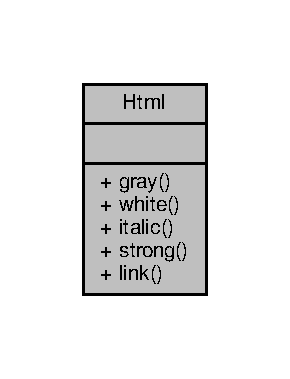
\includegraphics[width=139pt]{classHtml__coll__graph}
\end{center}
\end{figure}
\subsection*{Static Public Member Functions}
\begin{DoxyCompactItemize}
\item 
static Q\+String \hyperlink{classHtml_a4e22ddd91517477b1746f61b337f7d26}{gray} (Q\+String str)
\begin{DoxyCompactList}\small\item\em Make text gray. \end{DoxyCompactList}\item 
static Q\+String \hyperlink{classHtml_aa1ff559b97635462aef31a98f7277a53}{white} (Q\+String str)
\begin{DoxyCompactList}\small\item\em Make text white. \end{DoxyCompactList}\item 
static Q\+String \hyperlink{classHtml_a0c5391338202adb52475498e38143bb1}{italic} (Q\+String str)
\begin{DoxyCompactList}\small\item\em Make text italic. \end{DoxyCompactList}\item 
static Q\+String \hyperlink{classHtml_adf0b7c3aa257d977810e6f3a60e98e6a}{strong} (Q\+String str)
\begin{DoxyCompactList}\small\item\em Make text strong. \end{DoxyCompactList}\item 
static Q\+String \hyperlink{classHtml_a1a01e004b980594e5223db319b4677c6}{link} (Q\+String str)
\begin{DoxyCompactList}\small\item\em Make text to be link. \end{DoxyCompactList}\end{DoxyCompactItemize}


\subsection{Detailed Description}
Add H\+T\+ML flavor to a string. 

\subsection{Member Function Documentation}
\index{Html@{Html}!gray@{gray}}
\index{gray@{gray}!Html@{Html}}
\subsubsection[{\texorpdfstring{gray(\+Q\+String str)}{gray(QString str)}}]{\setlength{\rightskip}{0pt plus 5cm}Q\+String Html\+::gray (
\begin{DoxyParamCaption}
\item[{Q\+String}]{str}
\end{DoxyParamCaption}
)\hspace{0.3cm}{\ttfamily [static]}}\hypertarget{classHtml_a4e22ddd91517477b1746f61b337f7d26}{}\label{classHtml_a4e22ddd91517477b1746f61b337f7d26}


Make text gray. 

\index{Html@{Html}!italic@{italic}}
\index{italic@{italic}!Html@{Html}}
\subsubsection[{\texorpdfstring{italic(\+Q\+String str)}{italic(QString str)}}]{\setlength{\rightskip}{0pt plus 5cm}Q\+String Html\+::italic (
\begin{DoxyParamCaption}
\item[{Q\+String}]{str}
\end{DoxyParamCaption}
)\hspace{0.3cm}{\ttfamily [static]}}\hypertarget{classHtml_a0c5391338202adb52475498e38143bb1}{}\label{classHtml_a0c5391338202adb52475498e38143bb1}


Make text italic. 

\index{Html@{Html}!link@{link}}
\index{link@{link}!Html@{Html}}
\subsubsection[{\texorpdfstring{link(\+Q\+String str)}{link(QString str)}}]{\setlength{\rightskip}{0pt plus 5cm}Q\+String Html\+::link (
\begin{DoxyParamCaption}
\item[{Q\+String}]{str}
\end{DoxyParamCaption}
)\hspace{0.3cm}{\ttfamily [static]}}\hypertarget{classHtml_a1a01e004b980594e5223db319b4677c6}{}\label{classHtml_a1a01e004b980594e5223db319b4677c6}


Make text to be link. 

\index{Html@{Html}!strong@{strong}}
\index{strong@{strong}!Html@{Html}}
\subsubsection[{\texorpdfstring{strong(\+Q\+String str)}{strong(QString str)}}]{\setlength{\rightskip}{0pt plus 5cm}Q\+String Html\+::strong (
\begin{DoxyParamCaption}
\item[{Q\+String}]{str}
\end{DoxyParamCaption}
)\hspace{0.3cm}{\ttfamily [static]}}\hypertarget{classHtml_adf0b7c3aa257d977810e6f3a60e98e6a}{}\label{classHtml_adf0b7c3aa257d977810e6f3a60e98e6a}


Make text strong. 

\index{Html@{Html}!white@{white}}
\index{white@{white}!Html@{Html}}
\subsubsection[{\texorpdfstring{white(\+Q\+String str)}{white(QString str)}}]{\setlength{\rightskip}{0pt plus 5cm}Q\+String Html\+::white (
\begin{DoxyParamCaption}
\item[{Q\+String}]{str}
\end{DoxyParamCaption}
)\hspace{0.3cm}{\ttfamily [static]}}\hypertarget{classHtml_aa1ff559b97635462aef31a98f7277a53}{}\label{classHtml_aa1ff559b97635462aef31a98f7277a53}


Make text white. 



The documentation for this class was generated from the following files\+:\begin{DoxyCompactItemize}
\item 
\hyperlink{html_8h}{html.\+h}\item 
\hyperlink{html_8cpp}{html.\+cpp}\end{DoxyCompactItemize}

\hypertarget{classLabelWithClick}{}\section{Label\+With\+Click Class Reference}
\label{classLabelWithClick}\index{Label\+With\+Click@{Label\+With\+Click}}


{\ttfamily \#include $<$labelwithclick.\+h$>$}



Inheritance diagram for Label\+With\+Click\+:
\nopagebreak
\begin{figure}[H]
\begin{center}
\leavevmode
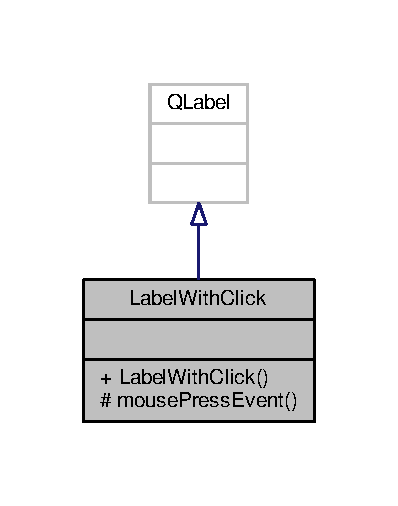
\includegraphics[width=191pt]{classLabelWithClick__inherit__graph}
\end{center}
\end{figure}


Collaboration diagram for Label\+With\+Click\+:
\nopagebreak
\begin{figure}[H]
\begin{center}
\leavevmode
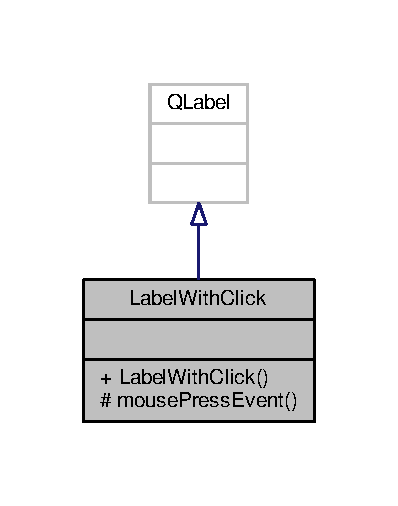
\includegraphics[width=191pt]{classLabelWithClick__coll__graph}
\end{center}
\end{figure}
\subsection*{Signals}
\begin{DoxyCompactItemize}
\item 
void \hyperlink{classLabelWithClick_ac539cd54276af3f36ea0729e998a7650}{clicked} ()
\end{DoxyCompactItemize}
\subsection*{Public Member Functions}
\begin{DoxyCompactItemize}
\item 
\hyperlink{classLabelWithClick_aa87365b48e3d45d968e522190dc8589f}{Label\+With\+Click} (const Q\+String \&text, Q\+Widget $\ast$parent=0)
\end{DoxyCompactItemize}
\subsection*{Protected Member Functions}
\begin{DoxyCompactItemize}
\item 
void \hyperlink{classLabelWithClick_a6b2f04ed99833bf8ef45d1ec1ad790e7}{mouse\+Press\+Event} (Q\+Mouse\+Event $\ast$event) override
\end{DoxyCompactItemize}


\subsection{Constructor \& Destructor Documentation}
\index{Label\+With\+Click@{Label\+With\+Click}!Label\+With\+Click@{Label\+With\+Click}}
\index{Label\+With\+Click@{Label\+With\+Click}!Label\+With\+Click@{Label\+With\+Click}}
\subsubsection[{\texorpdfstring{Label\+With\+Click(const Q\+String \&text, Q\+Widget $\ast$parent=0)}{LabelWithClick(const QString &text, QWidget *parent=0)}}]{\setlength{\rightskip}{0pt plus 5cm}Label\+With\+Click\+::\+Label\+With\+Click (
\begin{DoxyParamCaption}
\item[{const Q\+String \&}]{text, }
\item[{Q\+Widget $\ast$}]{parent = {\ttfamily 0}}
\end{DoxyParamCaption}
)\hspace{0.3cm}{\ttfamily [explicit]}}\hypertarget{classLabelWithClick_aa87365b48e3d45d968e522190dc8589f}{}\label{classLabelWithClick_aa87365b48e3d45d968e522190dc8589f}


\subsection{Member Function Documentation}
\index{Label\+With\+Click@{Label\+With\+Click}!clicked@{clicked}}
\index{clicked@{clicked}!Label\+With\+Click@{Label\+With\+Click}}
\subsubsection[{\texorpdfstring{clicked}{clicked}}]{\setlength{\rightskip}{0pt plus 5cm}void Label\+With\+Click\+::clicked (
\begin{DoxyParamCaption}
{}
\end{DoxyParamCaption}
)\hspace{0.3cm}{\ttfamily [signal]}}\hypertarget{classLabelWithClick_ac539cd54276af3f36ea0729e998a7650}{}\label{classLabelWithClick_ac539cd54276af3f36ea0729e998a7650}
\index{Label\+With\+Click@{Label\+With\+Click}!mouse\+Press\+Event@{mouse\+Press\+Event}}
\index{mouse\+Press\+Event@{mouse\+Press\+Event}!Label\+With\+Click@{Label\+With\+Click}}
\subsubsection[{\texorpdfstring{mouse\+Press\+Event(\+Q\+Mouse\+Event $\ast$event) override}{mousePressEvent(QMouseEvent *event) override}}]{\setlength{\rightskip}{0pt plus 5cm}void Label\+With\+Click\+::mouse\+Press\+Event (
\begin{DoxyParamCaption}
\item[{Q\+Mouse\+Event $\ast$}]{event}
\end{DoxyParamCaption}
)\hspace{0.3cm}{\ttfamily [override]}, {\ttfamily [protected]}}\hypertarget{classLabelWithClick_a6b2f04ed99833bf8ef45d1ec1ad790e7}{}\label{classLabelWithClick_a6b2f04ed99833bf8ef45d1ec1ad790e7}


The documentation for this class was generated from the following files\+:\begin{DoxyCompactItemize}
\item 
\hyperlink{labelwithclick_8h}{labelwithclick.\+h}\item 
\hyperlink{labelwithclick_8cpp}{labelwithclick.\+cpp}\end{DoxyCompactItemize}

\hypertarget{classMainWindow}{}\section{Main\+Window Class Reference}
\label{classMainWindow}\index{Main\+Window@{Main\+Window}}


{\ttfamily \#include $<$mainwindow.\+h$>$}



Inheritance diagram for Main\+Window\+:
\nopagebreak
\begin{figure}[H]
\begin{center}
\leavevmode
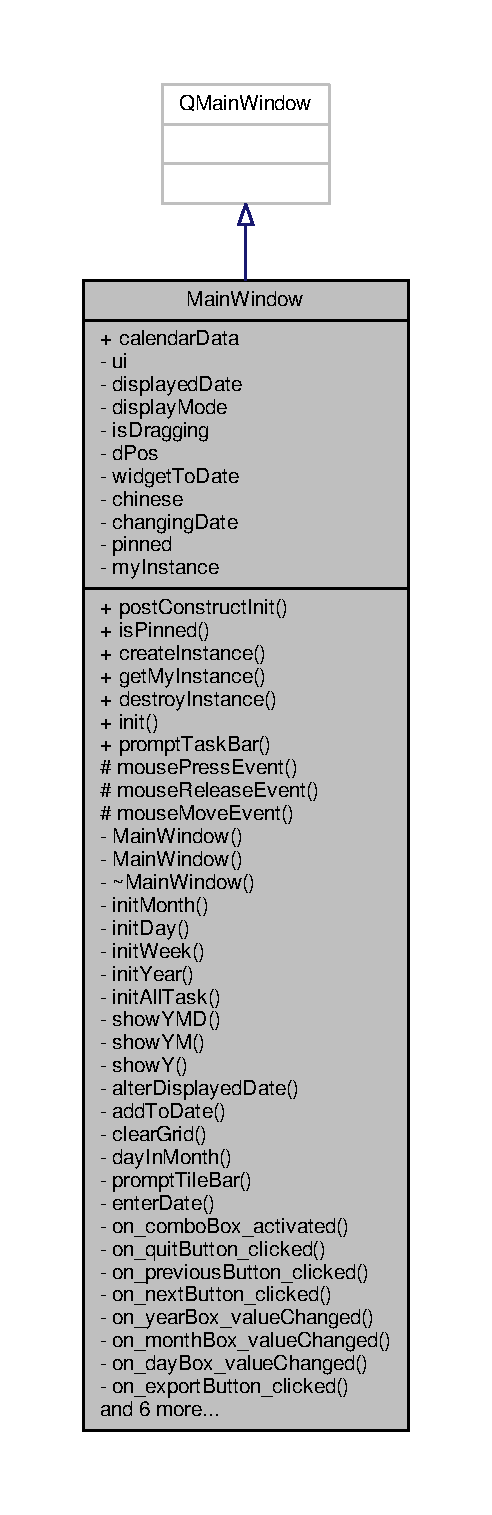
\includegraphics[height=550pt]{classMainWindow__inherit__graph}
\end{center}
\end{figure}


Collaboration diagram for Main\+Window\+:
\nopagebreak
\begin{figure}[H]
\begin{center}
\leavevmode
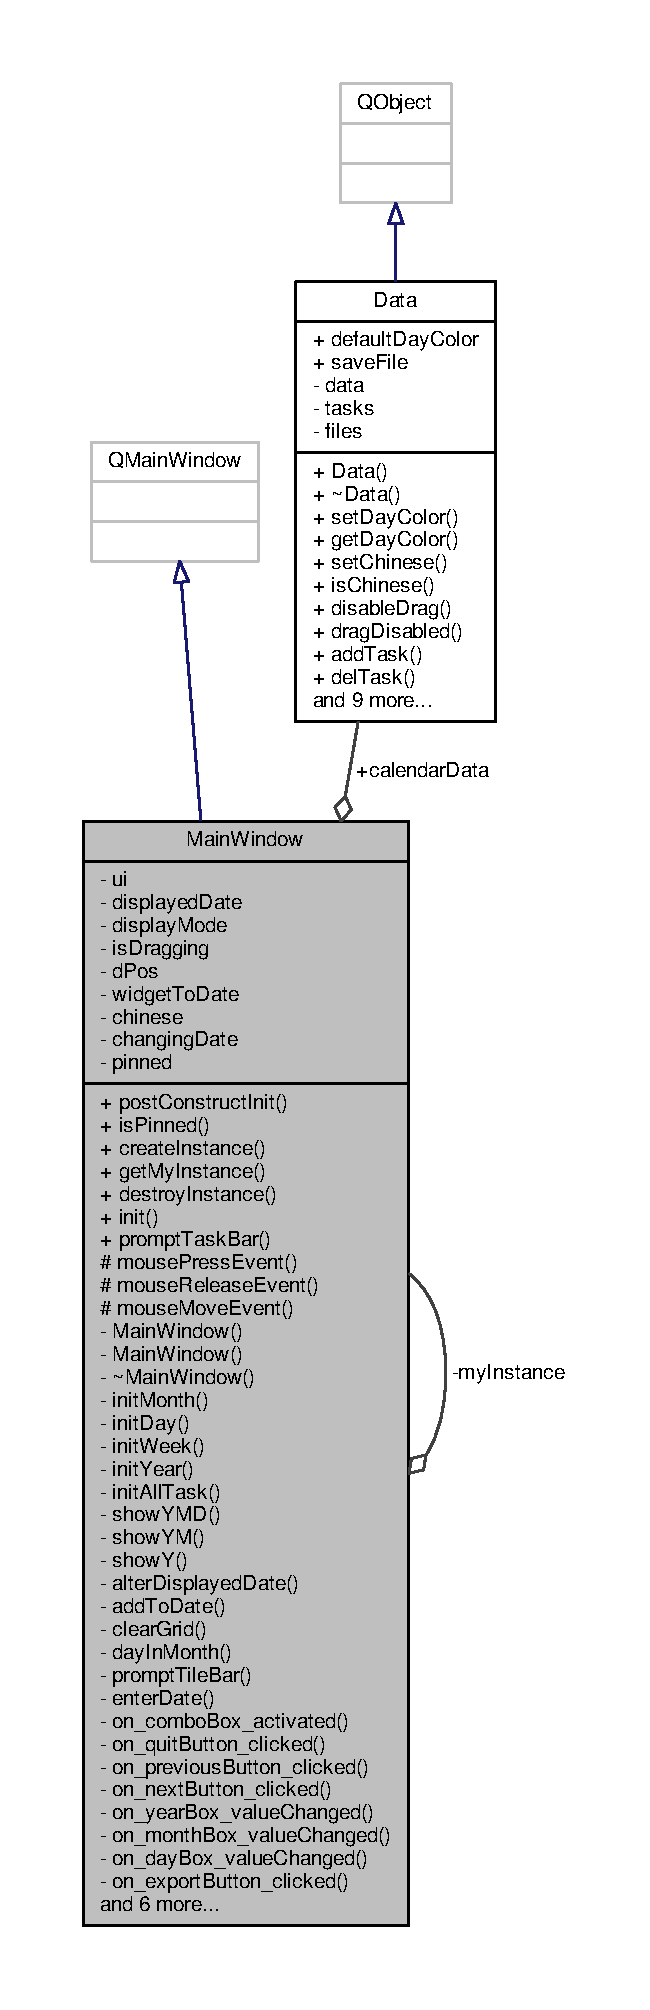
\includegraphics[height=550pt]{classMainWindow__coll__graph}
\end{center}
\end{figure}
\subsection*{Public Slots}
\begin{DoxyCompactItemize}
\item 
void \hyperlink{classMainWindow_a671e7e5b0a3a7a3fb1cf44c5c8377952}{init} ()
\begin{DoxyCompactList}\small\item\em Initialize or renew the main grid display. \end{DoxyCompactList}\item 
void \hyperlink{classMainWindow_a4c5f8ee24616439a17d368fe95ab6c41}{prompt\+Task\+Bar} (Q\+Widget $\ast$task, int task\+Index, Q\+Date today)
\end{DoxyCompactItemize}
\subsection*{Public Member Functions}
\begin{DoxyCompactItemize}
\item 
void \hyperlink{classMainWindow_a8566d13d3417aa595a1533586cc3ada5}{post\+Construct\+Init} ()
\begin{DoxyCompactList}\small\item\em Do some initialization that cannot be put into constructor. \end{DoxyCompactList}\item 
bool \hyperlink{classMainWindow_aae7db4c3a3f3e723ec3d21adb9ef7fd4}{is\+Pinned} () const 
\begin{DoxyCompactList}\small\item\em Whether to not response to mouse event. \end{DoxyCompactList}\end{DoxyCompactItemize}
\subsection*{Static Public Member Functions}
\begin{DoxyCompactItemize}
\item 
static void \hyperlink{classMainWindow_a9d383570468f2568c9637c799fb1dfe1}{create\+Instance} ()
\item 
static \hyperlink{classMainWindow}{Main\+Window} $\ast$ \hyperlink{classMainWindow_a5f4dcec4f4725d36109f6530e52a22af}{get\+My\+Instance} ()
\item 
static void \hyperlink{classMainWindow_a61c1442c562239ef28e3d77d00d2234c}{destroy\+Instance} ()
\end{DoxyCompactItemize}
\subsection*{Public Attributes}
\begin{DoxyCompactItemize}
\item 
\hyperlink{classData}{Data} $\ast$ \hyperlink{classMainWindow_a4344962e43608c8c9f1b03e98eaa9283}{calendar\+Data}
\begin{DoxyCompactList}\small\item\em All data set by user. \end{DoxyCompactList}\end{DoxyCompactItemize}
\subsection*{Protected Member Functions}
\begin{DoxyCompactItemize}
\item 
void \hyperlink{classMainWindow_a2b5463ae209a03d1680b39c950dac8be}{mouse\+Press\+Event} (Q\+Mouse\+Event $\ast$event)
\item 
void \hyperlink{classMainWindow_a32bbb036a55856e49c31a5348f937b53}{mouse\+Release\+Event} (Q\+Mouse\+Event $\ast$event)
\item 
void \hyperlink{classMainWindow_a2cf42454562815dd44c716e78d515697}{mouse\+Move\+Event} (Q\+Mouse\+Event $\ast$event)
\end{DoxyCompactItemize}
\subsection*{Private Types}
\begin{DoxyCompactItemize}
\item 
enum \hyperlink{classMainWindow_a32a99bf8f548bef64c48491cfa6225e8}{Display\+Mode} \{ \\*
\hyperlink{classMainWindow_a32a99bf8f548bef64c48491cfa6225e8ae246ce36606e3dcc90557e03ff0f56d3}{M\+O\+N\+TH} = 0, 
\hyperlink{classMainWindow_a32a99bf8f548bef64c48491cfa6225e8aace7e7f9db7ef6ea0e1035adb1cd7816}{D\+AY} = 1, 
\hyperlink{classMainWindow_a32a99bf8f548bef64c48491cfa6225e8ac595bfa80e486bcacb7156545d455220}{W\+E\+EK} = 2, 
\hyperlink{classMainWindow_a32a99bf8f548bef64c48491cfa6225e8abfec19a213e559fa1510f6470839dd54}{Y\+E\+AR} = 3, 
\\*
\hyperlink{classMainWindow_a32a99bf8f548bef64c48491cfa6225e8a115c6a291d5706194267a4dfc6ce0d73}{T\+A\+SK} = 4
 \}
\end{DoxyCompactItemize}
\subsection*{Private Slots}
\begin{DoxyCompactItemize}
\item 
void \hyperlink{classMainWindow_a0b149c5bca3c35a39c919fe9581be2dd}{prompt\+Tile\+Bar} (Q\+Widget $\ast$tile)
\item 
void \hyperlink{classMainWindow_a407c21579299391a8d3e34f5b3af362e}{enter\+Date} (const Q\+Date \&date)
\item 
void \hyperlink{classMainWindow_a20dbb80de6c861f26ae88c4588ca6cf2}{on\+\_\+combo\+Box\+\_\+activated} (int index)
\item 
void \hyperlink{classMainWindow_aca2f10b04ded003c6da32e81c898d16e}{on\+\_\+quit\+Button\+\_\+clicked} (bool checked)
\item 
void \hyperlink{classMainWindow_a228228aec016d5f37ef06dc62ad0c42a}{on\+\_\+previous\+Button\+\_\+clicked} (bool checked)
\item 
void \hyperlink{classMainWindow_ad1a550b59a2a3a2a0b48f2f63e8071eb}{on\+\_\+next\+Button\+\_\+clicked} (bool checked)
\item 
void \hyperlink{classMainWindow_a906e1abeb5bda05405106d78779872e3}{on\+\_\+year\+Box\+\_\+value\+Changed} (int arg1)
\item 
void \hyperlink{classMainWindow_a369ef8f03c1c6e986418234bd462ab06}{on\+\_\+month\+Box\+\_\+value\+Changed} (int arg1)
\item 
void \hyperlink{classMainWindow_ac985b15a3e2b9a28ca2e319fb039d1d7}{on\+\_\+day\+Box\+\_\+value\+Changed} (int arg1)
\item 
void \hyperlink{classMainWindow_a0ae56967e1df87215428eb9f91df9ba0}{on\+\_\+export\+Button\+\_\+clicked} (bool checked)
\item 
void \hyperlink{classMainWindow_a42193cb2a4a2cac74da5a8291ab5bd96}{on\+\_\+import\+Button\+\_\+clicked} (bool checked)
\item 
void \hyperlink{classMainWindow_ae779988974613e15ccb434645f474d8f}{on\+\_\+pin\+Button\+\_\+clicked} (bool checked)
\item 
void \hyperlink{classMainWindow_a9e6103352c52b8e96959a71919ad4cf9}{on\+\_\+drag\+Switch\+Button\+\_\+clicked} (bool checked)
\item 
void \hyperlink{classMainWindow_a0679e38138ca8bfdf6a877cbc821b21b}{on\+\_\+drag\+Switch\+Button\+\_\+toggled} (bool checked)
\item 
void \hyperlink{classMainWindow_a4cd877b54dd972c62fa97553191d69c1}{on\+\_\+mode\+Box\+\_\+activated} (int index)
\item 
void \hyperlink{classMainWindow_af5c3bae5874c9868604a90ee6071cc04}{on\+\_\+help\+Button\+\_\+clicked} (bool checked)
\end{DoxyCompactItemize}
\subsection*{Private Member Functions}
\begin{DoxyCompactItemize}
\item 
\hyperlink{classMainWindow_a8b244be8b7b7db1b08de2a2acb9409db}{Main\+Window} (Q\+Widget $\ast$parent=0)
\item 
\hyperlink{classMainWindow_af1d822d2183a379458e4bc0e2ea2bf3b}{Main\+Window} (const \hyperlink{classMainWindow}{Main\+Window} \&)=delete
\item 
\hyperlink{classMainWindow_ae98d00a93bc118200eeef9f9bba1dba7}{$\sim$\+Main\+Window} ()
\item 
void \hyperlink{classMainWindow_a6ae0984b3c00fe9253616e9f5aeea6d2}{init\+Month} ()
\begin{DoxyCompactList}\small\item\em Initialize a month display. \end{DoxyCompactList}\item 
void \hyperlink{classMainWindow_adcc14141e6eef45ee903900bb83f8129}{init\+Day} ()
\begin{DoxyCompactList}\small\item\em Initialize a day display. \end{DoxyCompactList}\item 
void \hyperlink{classMainWindow_ae7ea21dab9b67f4a691c798026b61999}{init\+Week} ()
\begin{DoxyCompactList}\small\item\em Initialize a week display. \end{DoxyCompactList}\item 
void \hyperlink{classMainWindow_a8791b87648ba02f9f40ff0e4d820a76a}{init\+Year} ()
\begin{DoxyCompactList}\small\item\em Initialize a year display. \end{DoxyCompactList}\item 
void \hyperlink{classMainWindow_a9019bfe47aed0dd0d9c6647e066eb55e}{init\+All\+Task} ()
\begin{DoxyCompactList}\small\item\em Initialize a all-\/tasks display. i.\+e. all the days that have tasks or files. \end{DoxyCompactList}\item 
void \hyperlink{classMainWindow_aa2a16a8bde8f4d34b1f5c333a7c6041f}{show\+Y\+MD} ()
\begin{DoxyCompactList}\small\item\em These 3 functions set the date bar at top. \end{DoxyCompactList}\item 
void \hyperlink{classMainWindow_a6c1803c0b3b3299044eb2d33bc9c0e7d}{show\+YM} ()
\begin{DoxyCompactList}\small\item\em year \& month \& day \end{DoxyCompactList}\item 
void \hyperlink{classMainWindow_ad779c7052af374e51a7f3a2259874df1}{showY} ()
\begin{DoxyCompactList}\small\item\em year \& month \end{DoxyCompactList}\item 
void \hyperlink{classMainWindow_adfb23ac3d671ce0d029139658d9bf7d3}{alter\+Displayed\+Date} (Q\+Date date)
\begin{DoxyCompactList}\small\item\em year \end{DoxyCompactList}\item 
void \hyperlink{classMainWindow_af7232133bb63540bf0c30b419c36b7d0}{add\+To\+Date} (int x)
\begin{DoxyCompactList}\small\item\em Add an interval x to current displayed date. \end{DoxyCompactList}\item 
void \hyperlink{classMainWindow_a5e43be8d8c2c6a2c5a4a73d764cac47b}{clear\+Grid} ()
\begin{DoxyCompactList}\small\item\em Clear all cells in the grid. \end{DoxyCompactList}\item 
Q\+Widget $\ast$ \hyperlink{classMainWindow_a99a20813bb08b5c93c33f20255f73c67}{day\+In\+Month} (Q\+Date date, bool month\+Displayed)
\begin{DoxyCompactList}\small\item\em Generates a cell for a day. \end{DoxyCompactList}\end{DoxyCompactItemize}
\subsection*{Private Attributes}
\begin{DoxyCompactItemize}
\item 
Ui\+::\+Main\+Window $\ast$ \hyperlink{classMainWindow_a35466a70ed47252a0191168126a352a5}{ui}
\item 
Q\+Date \hyperlink{classMainWindow_a3d53fc161132967689d4dde0ad7f8a21}{displayed\+Date}
\begin{DoxyCompactList}\small\item\em date displayed in the main window \end{DoxyCompactList}\item 
enum \hyperlink{classMainWindow_a32a99bf8f548bef64c48491cfa6225e8}{Main\+Window\+::\+Display\+Mode} \hyperlink{classMainWindow_a3408763a676b4754ed8f3de394d9c70b}{display\+Mode}
\item 
bool \hyperlink{classMainWindow_ab664d23548b84c308cc3809c1e63aaff}{is\+Dragging}
\begin{DoxyCompactList}\small\item\em is dragging window \end{DoxyCompactList}\item 
Q\+Point \hyperlink{classMainWindow_a98499e8e85458e2dc2ac349964230983}{d\+Pos}
\begin{DoxyCompactList}\small\item\em Original pos for moving the window. \end{DoxyCompactList}\item 
Q\+Map$<$ Q\+Widget $\ast$, Q\+Date $>$ \hyperlink{classMainWindow_ae81ee3cac7678dba0be2fcc37949daa7}{widget\+To\+Date}
\begin{DoxyCompactList}\small\item\em What wiget refers to what date. \end{DoxyCompactList}\item 
Q\+Translator \hyperlink{classMainWindow_a2c428c740faa1094e20f658b2db84dc7}{chinese}
\item 
bool \hyperlink{classMainWindow_a4ba1fa11c17bc9919783f8988f0f6e92}{changing\+Date}
\begin{DoxyCompactList}\small\item\em Prevent recursive calling. \end{DoxyCompactList}\item 
bool \hyperlink{classMainWindow_aac8447a932ef41f544891a8d74d04ab9}{pinned}
\begin{DoxyCompactList}\small\item\em The grid not reveiving mouse event. \end{DoxyCompactList}\end{DoxyCompactItemize}
\subsection*{Static Private Attributes}
\begin{DoxyCompactItemize}
\item 
static \hyperlink{classMainWindow}{Main\+Window} $\ast$ \hyperlink{classMainWindow_a40d454c031dd2ff6a4813fb298c79905}{my\+Instance} = 0
\end{DoxyCompactItemize}


\subsection{Member Enumeration Documentation}
\index{Main\+Window@{Main\+Window}!Display\+Mode@{Display\+Mode}}
\index{Display\+Mode@{Display\+Mode}!Main\+Window@{Main\+Window}}
\subsubsection[{\texorpdfstring{Display\+Mode}{DisplayMode}}]{\setlength{\rightskip}{0pt plus 5cm}enum {\bf Main\+Window\+::\+Display\+Mode}\hspace{0.3cm}{\ttfamily [private]}}\hypertarget{classMainWindow_a32a99bf8f548bef64c48491cfa6225e8}{}\label{classMainWindow_a32a99bf8f548bef64c48491cfa6225e8}
\begin{Desc}
\item[Enumerator]\par
\begin{description}
\index{M\+O\+N\+TH@{M\+O\+N\+TH}!Main\+Window@{Main\+Window}}\index{Main\+Window@{Main\+Window}!M\+O\+N\+TH@{M\+O\+N\+TH}}\item[{\em 
M\+O\+N\+TH\hypertarget{classMainWindow_a32a99bf8f548bef64c48491cfa6225e8ae246ce36606e3dcc90557e03ff0f56d3}{}\label{classMainWindow_a32a99bf8f548bef64c48491cfa6225e8ae246ce36606e3dcc90557e03ff0f56d3}
}]\index{D\+AY@{D\+AY}!Main\+Window@{Main\+Window}}\index{Main\+Window@{Main\+Window}!D\+AY@{D\+AY}}\item[{\em 
D\+AY\hypertarget{classMainWindow_a32a99bf8f548bef64c48491cfa6225e8aace7e7f9db7ef6ea0e1035adb1cd7816}{}\label{classMainWindow_a32a99bf8f548bef64c48491cfa6225e8aace7e7f9db7ef6ea0e1035adb1cd7816}
}]\index{W\+E\+EK@{W\+E\+EK}!Main\+Window@{Main\+Window}}\index{Main\+Window@{Main\+Window}!W\+E\+EK@{W\+E\+EK}}\item[{\em 
W\+E\+EK\hypertarget{classMainWindow_a32a99bf8f548bef64c48491cfa6225e8ac595bfa80e486bcacb7156545d455220}{}\label{classMainWindow_a32a99bf8f548bef64c48491cfa6225e8ac595bfa80e486bcacb7156545d455220}
}]\index{Y\+E\+AR@{Y\+E\+AR}!Main\+Window@{Main\+Window}}\index{Main\+Window@{Main\+Window}!Y\+E\+AR@{Y\+E\+AR}}\item[{\em 
Y\+E\+AR\hypertarget{classMainWindow_a32a99bf8f548bef64c48491cfa6225e8abfec19a213e559fa1510f6470839dd54}{}\label{classMainWindow_a32a99bf8f548bef64c48491cfa6225e8abfec19a213e559fa1510f6470839dd54}
}]\index{T\+A\+SK@{T\+A\+SK}!Main\+Window@{Main\+Window}}\index{Main\+Window@{Main\+Window}!T\+A\+SK@{T\+A\+SK}}\item[{\em 
T\+A\+SK\hypertarget{classMainWindow_a32a99bf8f548bef64c48491cfa6225e8a115c6a291d5706194267a4dfc6ce0d73}{}\label{classMainWindow_a32a99bf8f548bef64c48491cfa6225e8a115c6a291d5706194267a4dfc6ce0d73}
}]\end{description}
\end{Desc}


\subsection{Constructor \& Destructor Documentation}
\index{Main\+Window@{Main\+Window}!Main\+Window@{Main\+Window}}
\index{Main\+Window@{Main\+Window}!Main\+Window@{Main\+Window}}
\subsubsection[{\texorpdfstring{Main\+Window(\+Q\+Widget $\ast$parent=0)}{MainWindow(QWidget *parent=0)}}]{\setlength{\rightskip}{0pt plus 5cm}Main\+Window\+::\+Main\+Window (
\begin{DoxyParamCaption}
\item[{Q\+Widget $\ast$}]{parent = {\ttfamily 0}}
\end{DoxyParamCaption}
)\hspace{0.3cm}{\ttfamily [explicit]}, {\ttfamily [private]}}\hypertarget{classMainWindow_a8b244be8b7b7db1b08de2a2acb9409db}{}\label{classMainWindow_a8b244be8b7b7db1b08de2a2acb9409db}
\index{Main\+Window@{Main\+Window}!Main\+Window@{Main\+Window}}
\index{Main\+Window@{Main\+Window}!Main\+Window@{Main\+Window}}
\subsubsection[{\texorpdfstring{Main\+Window(const Main\+Window \&)=delete}{MainWindow(const MainWindow &)=delete}}]{\setlength{\rightskip}{0pt plus 5cm}Main\+Window\+::\+Main\+Window (
\begin{DoxyParamCaption}
\item[{const {\bf Main\+Window} \&}]{}
\end{DoxyParamCaption}
)\hspace{0.3cm}{\ttfamily [private]}, {\ttfamily [delete]}}\hypertarget{classMainWindow_af1d822d2183a379458e4bc0e2ea2bf3b}{}\label{classMainWindow_af1d822d2183a379458e4bc0e2ea2bf3b}
\index{Main\+Window@{Main\+Window}!````~Main\+Window@{$\sim$\+Main\+Window}}
\index{````~Main\+Window@{$\sim$\+Main\+Window}!Main\+Window@{Main\+Window}}
\subsubsection[{\texorpdfstring{$\sim$\+Main\+Window()}{~MainWindow()}}]{\setlength{\rightskip}{0pt plus 5cm}Main\+Window\+::$\sim$\+Main\+Window (
\begin{DoxyParamCaption}
{}
\end{DoxyParamCaption}
)\hspace{0.3cm}{\ttfamily [private]}}\hypertarget{classMainWindow_ae98d00a93bc118200eeef9f9bba1dba7}{}\label{classMainWindow_ae98d00a93bc118200eeef9f9bba1dba7}


\subsection{Member Function Documentation}
\index{Main\+Window@{Main\+Window}!add\+To\+Date@{add\+To\+Date}}
\index{add\+To\+Date@{add\+To\+Date}!Main\+Window@{Main\+Window}}
\subsubsection[{\texorpdfstring{add\+To\+Date(int x)}{addToDate(int x)}}]{\setlength{\rightskip}{0pt plus 5cm}void Main\+Window\+::add\+To\+Date (
\begin{DoxyParamCaption}
\item[{int}]{x}
\end{DoxyParamCaption}
)\hspace{0.3cm}{\ttfamily [private]}}\hypertarget{classMainWindow_af7232133bb63540bf0c30b419c36b7d0}{}\label{classMainWindow_af7232133bb63540bf0c30b419c36b7d0}


Add an interval x to current displayed date. 

\index{Main\+Window@{Main\+Window}!alter\+Displayed\+Date@{alter\+Displayed\+Date}}
\index{alter\+Displayed\+Date@{alter\+Displayed\+Date}!Main\+Window@{Main\+Window}}
\subsubsection[{\texorpdfstring{alter\+Displayed\+Date(\+Q\+Date date)}{alterDisplayedDate(QDate date)}}]{\setlength{\rightskip}{0pt plus 5cm}void Main\+Window\+::alter\+Displayed\+Date (
\begin{DoxyParamCaption}
\item[{Q\+Date}]{date}
\end{DoxyParamCaption}
)\hspace{0.3cm}{\ttfamily [private]}}\hypertarget{classMainWindow_adfb23ac3d671ce0d029139658d9bf7d3}{}\label{classMainWindow_adfb23ac3d671ce0d029139658d9bf7d3}


year 

Display another date \index{Main\+Window@{Main\+Window}!clear\+Grid@{clear\+Grid}}
\index{clear\+Grid@{clear\+Grid}!Main\+Window@{Main\+Window}}
\subsubsection[{\texorpdfstring{clear\+Grid()}{clearGrid()}}]{\setlength{\rightskip}{0pt plus 5cm}void Main\+Window\+::clear\+Grid (
\begin{DoxyParamCaption}
{}
\end{DoxyParamCaption}
)\hspace{0.3cm}{\ttfamily [private]}}\hypertarget{classMainWindow_a5e43be8d8c2c6a2c5a4a73d764cac47b}{}\label{classMainWindow_a5e43be8d8c2c6a2c5a4a73d764cac47b}


Clear all cells in the grid. 

\index{Main\+Window@{Main\+Window}!create\+Instance@{create\+Instance}}
\index{create\+Instance@{create\+Instance}!Main\+Window@{Main\+Window}}
\subsubsection[{\texorpdfstring{create\+Instance()}{createInstance()}}]{\setlength{\rightskip}{0pt plus 5cm}void Main\+Window\+::create\+Instance (
\begin{DoxyParamCaption}
{}
\end{DoxyParamCaption}
)\hspace{0.3cm}{\ttfamily [static]}}\hypertarget{classMainWindow_a9d383570468f2568c9637c799fb1dfe1}{}\label{classMainWindow_a9d383570468f2568c9637c799fb1dfe1}
\index{Main\+Window@{Main\+Window}!day\+In\+Month@{day\+In\+Month}}
\index{day\+In\+Month@{day\+In\+Month}!Main\+Window@{Main\+Window}}
\subsubsection[{\texorpdfstring{day\+In\+Month(\+Q\+Date date, bool month\+Displayed)}{dayInMonth(QDate date, bool monthDisplayed)}}]{\setlength{\rightskip}{0pt plus 5cm}Q\+Widget $\ast$ Main\+Window\+::day\+In\+Month (
\begin{DoxyParamCaption}
\item[{Q\+Date}]{date, }
\item[{bool}]{month\+Displayed}
\end{DoxyParamCaption}
)\hspace{0.3cm}{\ttfamily [private]}}\hypertarget{classMainWindow_a99a20813bb08b5c93c33f20255f73c67}{}\label{classMainWindow_a99a20813bb08b5c93c33f20255f73c67}


Generates a cell for a day. 

\index{Main\+Window@{Main\+Window}!destroy\+Instance@{destroy\+Instance}}
\index{destroy\+Instance@{destroy\+Instance}!Main\+Window@{Main\+Window}}
\subsubsection[{\texorpdfstring{destroy\+Instance()}{destroyInstance()}}]{\setlength{\rightskip}{0pt plus 5cm}void Main\+Window\+::destroy\+Instance (
\begin{DoxyParamCaption}
{}
\end{DoxyParamCaption}
)\hspace{0.3cm}{\ttfamily [static]}}\hypertarget{classMainWindow_a61c1442c562239ef28e3d77d00d2234c}{}\label{classMainWindow_a61c1442c562239ef28e3d77d00d2234c}
\index{Main\+Window@{Main\+Window}!enter\+Date@{enter\+Date}}
\index{enter\+Date@{enter\+Date}!Main\+Window@{Main\+Window}}
\subsubsection[{\texorpdfstring{enter\+Date}{enterDate}}]{\setlength{\rightskip}{0pt plus 5cm}void Main\+Window\+::enter\+Date (
\begin{DoxyParamCaption}
\item[{const Q\+Date \&}]{date}
\end{DoxyParamCaption}
)\hspace{0.3cm}{\ttfamily [private]}, {\ttfamily [slot]}}\hypertarget{classMainWindow_a407c21579299391a8d3e34f5b3af362e}{}\label{classMainWindow_a407c21579299391a8d3e34f5b3af362e}
\index{Main\+Window@{Main\+Window}!get\+My\+Instance@{get\+My\+Instance}}
\index{get\+My\+Instance@{get\+My\+Instance}!Main\+Window@{Main\+Window}}
\subsubsection[{\texorpdfstring{get\+My\+Instance()}{getMyInstance()}}]{\setlength{\rightskip}{0pt plus 5cm}{\bf Main\+Window} $\ast$ Main\+Window\+::get\+My\+Instance (
\begin{DoxyParamCaption}
{}
\end{DoxyParamCaption}
)\hspace{0.3cm}{\ttfamily [static]}}\hypertarget{classMainWindow_a5f4dcec4f4725d36109f6530e52a22af}{}\label{classMainWindow_a5f4dcec4f4725d36109f6530e52a22af}
\index{Main\+Window@{Main\+Window}!init@{init}}
\index{init@{init}!Main\+Window@{Main\+Window}}
\subsubsection[{\texorpdfstring{init}{init}}]{\setlength{\rightskip}{0pt plus 5cm}void Main\+Window\+::init (
\begin{DoxyParamCaption}
{}
\end{DoxyParamCaption}
)\hspace{0.3cm}{\ttfamily [slot]}}\hypertarget{classMainWindow_a671e7e5b0a3a7a3fb1cf44c5c8377952}{}\label{classMainWindow_a671e7e5b0a3a7a3fb1cf44c5c8377952}


Initialize or renew the main grid display. 

\index{Main\+Window@{Main\+Window}!init\+All\+Task@{init\+All\+Task}}
\index{init\+All\+Task@{init\+All\+Task}!Main\+Window@{Main\+Window}}
\subsubsection[{\texorpdfstring{init\+All\+Task()}{initAllTask()}}]{\setlength{\rightskip}{0pt plus 5cm}void Main\+Window\+::init\+All\+Task (
\begin{DoxyParamCaption}
{}
\end{DoxyParamCaption}
)\hspace{0.3cm}{\ttfamily [private]}}\hypertarget{classMainWindow_a9019bfe47aed0dd0d9c6647e066eb55e}{}\label{classMainWindow_a9019bfe47aed0dd0d9c6647e066eb55e}


Initialize a all-\/tasks display. i.\+e. all the days that have tasks or files. 

\index{Main\+Window@{Main\+Window}!init\+Day@{init\+Day}}
\index{init\+Day@{init\+Day}!Main\+Window@{Main\+Window}}
\subsubsection[{\texorpdfstring{init\+Day()}{initDay()}}]{\setlength{\rightskip}{0pt plus 5cm}void Main\+Window\+::init\+Day (
\begin{DoxyParamCaption}
{}
\end{DoxyParamCaption}
)\hspace{0.3cm}{\ttfamily [private]}}\hypertarget{classMainWindow_adcc14141e6eef45ee903900bb83f8129}{}\label{classMainWindow_adcc14141e6eef45ee903900bb83f8129}


Initialize a day display. 

\index{Main\+Window@{Main\+Window}!init\+Month@{init\+Month}}
\index{init\+Month@{init\+Month}!Main\+Window@{Main\+Window}}
\subsubsection[{\texorpdfstring{init\+Month()}{initMonth()}}]{\setlength{\rightskip}{0pt plus 5cm}void Main\+Window\+::init\+Month (
\begin{DoxyParamCaption}
{}
\end{DoxyParamCaption}
)\hspace{0.3cm}{\ttfamily [private]}}\hypertarget{classMainWindow_a6ae0984b3c00fe9253616e9f5aeea6d2}{}\label{classMainWindow_a6ae0984b3c00fe9253616e9f5aeea6d2}


Initialize a month display. 

\index{Main\+Window@{Main\+Window}!init\+Week@{init\+Week}}
\index{init\+Week@{init\+Week}!Main\+Window@{Main\+Window}}
\subsubsection[{\texorpdfstring{init\+Week()}{initWeek()}}]{\setlength{\rightskip}{0pt plus 5cm}void Main\+Window\+::init\+Week (
\begin{DoxyParamCaption}
{}
\end{DoxyParamCaption}
)\hspace{0.3cm}{\ttfamily [private]}}\hypertarget{classMainWindow_ae7ea21dab9b67f4a691c798026b61999}{}\label{classMainWindow_ae7ea21dab9b67f4a691c798026b61999}


Initialize a week display. 

\index{Main\+Window@{Main\+Window}!init\+Year@{init\+Year}}
\index{init\+Year@{init\+Year}!Main\+Window@{Main\+Window}}
\subsubsection[{\texorpdfstring{init\+Year()}{initYear()}}]{\setlength{\rightskip}{0pt plus 5cm}void Main\+Window\+::init\+Year (
\begin{DoxyParamCaption}
{}
\end{DoxyParamCaption}
)\hspace{0.3cm}{\ttfamily [private]}}\hypertarget{classMainWindow_a8791b87648ba02f9f40ff0e4d820a76a}{}\label{classMainWindow_a8791b87648ba02f9f40ff0e4d820a76a}


Initialize a year display. 

\index{Main\+Window@{Main\+Window}!is\+Pinned@{is\+Pinned}}
\index{is\+Pinned@{is\+Pinned}!Main\+Window@{Main\+Window}}
\subsubsection[{\texorpdfstring{is\+Pinned() const }{isPinned() const }}]{\setlength{\rightskip}{0pt plus 5cm}bool Main\+Window\+::is\+Pinned (
\begin{DoxyParamCaption}
{}
\end{DoxyParamCaption}
) const\hspace{0.3cm}{\ttfamily [inline]}}\hypertarget{classMainWindow_aae7db4c3a3f3e723ec3d21adb9ef7fd4}{}\label{classMainWindow_aae7db4c3a3f3e723ec3d21adb9ef7fd4}


Whether to not response to mouse event. 

\index{Main\+Window@{Main\+Window}!mouse\+Move\+Event@{mouse\+Move\+Event}}
\index{mouse\+Move\+Event@{mouse\+Move\+Event}!Main\+Window@{Main\+Window}}
\subsubsection[{\texorpdfstring{mouse\+Move\+Event(\+Q\+Mouse\+Event $\ast$event)}{mouseMoveEvent(QMouseEvent *event)}}]{\setlength{\rightskip}{0pt plus 5cm}void Main\+Window\+::mouse\+Move\+Event (
\begin{DoxyParamCaption}
\item[{Q\+Mouse\+Event $\ast$}]{event}
\end{DoxyParamCaption}
)\hspace{0.3cm}{\ttfamily [protected]}}\hypertarget{classMainWindow_a2cf42454562815dd44c716e78d515697}{}\label{classMainWindow_a2cf42454562815dd44c716e78d515697}
\index{Main\+Window@{Main\+Window}!mouse\+Press\+Event@{mouse\+Press\+Event}}
\index{mouse\+Press\+Event@{mouse\+Press\+Event}!Main\+Window@{Main\+Window}}
\subsubsection[{\texorpdfstring{mouse\+Press\+Event(\+Q\+Mouse\+Event $\ast$event)}{mousePressEvent(QMouseEvent *event)}}]{\setlength{\rightskip}{0pt plus 5cm}void Main\+Window\+::mouse\+Press\+Event (
\begin{DoxyParamCaption}
\item[{Q\+Mouse\+Event $\ast$}]{event}
\end{DoxyParamCaption}
)\hspace{0.3cm}{\ttfamily [protected]}}\hypertarget{classMainWindow_a2b5463ae209a03d1680b39c950dac8be}{}\label{classMainWindow_a2b5463ae209a03d1680b39c950dac8be}
\index{Main\+Window@{Main\+Window}!mouse\+Release\+Event@{mouse\+Release\+Event}}
\index{mouse\+Release\+Event@{mouse\+Release\+Event}!Main\+Window@{Main\+Window}}
\subsubsection[{\texorpdfstring{mouse\+Release\+Event(\+Q\+Mouse\+Event $\ast$event)}{mouseReleaseEvent(QMouseEvent *event)}}]{\setlength{\rightskip}{0pt plus 5cm}void Main\+Window\+::mouse\+Release\+Event (
\begin{DoxyParamCaption}
\item[{Q\+Mouse\+Event $\ast$}]{event}
\end{DoxyParamCaption}
)\hspace{0.3cm}{\ttfamily [protected]}}\hypertarget{classMainWindow_a32bbb036a55856e49c31a5348f937b53}{}\label{classMainWindow_a32bbb036a55856e49c31a5348f937b53}
\index{Main\+Window@{Main\+Window}!on\+\_\+combo\+Box\+\_\+activated@{on\+\_\+combo\+Box\+\_\+activated}}
\index{on\+\_\+combo\+Box\+\_\+activated@{on\+\_\+combo\+Box\+\_\+activated}!Main\+Window@{Main\+Window}}
\subsubsection[{\texorpdfstring{on\+\_\+combo\+Box\+\_\+activated}{on_comboBox_activated}}]{\setlength{\rightskip}{0pt plus 5cm}void Main\+Window\+::on\+\_\+combo\+Box\+\_\+activated (
\begin{DoxyParamCaption}
\item[{int}]{index}
\end{DoxyParamCaption}
)\hspace{0.3cm}{\ttfamily [private]}, {\ttfamily [slot]}}\hypertarget{classMainWindow_a20dbb80de6c861f26ae88c4588ca6cf2}{}\label{classMainWindow_a20dbb80de6c861f26ae88c4588ca6cf2}
\index{Main\+Window@{Main\+Window}!on\+\_\+day\+Box\+\_\+value\+Changed@{on\+\_\+day\+Box\+\_\+value\+Changed}}
\index{on\+\_\+day\+Box\+\_\+value\+Changed@{on\+\_\+day\+Box\+\_\+value\+Changed}!Main\+Window@{Main\+Window}}
\subsubsection[{\texorpdfstring{on\+\_\+day\+Box\+\_\+value\+Changed}{on_dayBox_valueChanged}}]{\setlength{\rightskip}{0pt plus 5cm}void Main\+Window\+::on\+\_\+day\+Box\+\_\+value\+Changed (
\begin{DoxyParamCaption}
\item[{int}]{arg1}
\end{DoxyParamCaption}
)\hspace{0.3cm}{\ttfamily [private]}, {\ttfamily [slot]}}\hypertarget{classMainWindow_ac985b15a3e2b9a28ca2e319fb039d1d7}{}\label{classMainWindow_ac985b15a3e2b9a28ca2e319fb039d1d7}
\index{Main\+Window@{Main\+Window}!on\+\_\+drag\+Switch\+Button\+\_\+clicked@{on\+\_\+drag\+Switch\+Button\+\_\+clicked}}
\index{on\+\_\+drag\+Switch\+Button\+\_\+clicked@{on\+\_\+drag\+Switch\+Button\+\_\+clicked}!Main\+Window@{Main\+Window}}
\subsubsection[{\texorpdfstring{on\+\_\+drag\+Switch\+Button\+\_\+clicked}{on_dragSwitchButton_clicked}}]{\setlength{\rightskip}{0pt plus 5cm}void Main\+Window\+::on\+\_\+drag\+Switch\+Button\+\_\+clicked (
\begin{DoxyParamCaption}
\item[{bool}]{checked}
\end{DoxyParamCaption}
)\hspace{0.3cm}{\ttfamily [private]}, {\ttfamily [slot]}}\hypertarget{classMainWindow_a9e6103352c52b8e96959a71919ad4cf9}{}\label{classMainWindow_a9e6103352c52b8e96959a71919ad4cf9}
\index{Main\+Window@{Main\+Window}!on\+\_\+drag\+Switch\+Button\+\_\+toggled@{on\+\_\+drag\+Switch\+Button\+\_\+toggled}}
\index{on\+\_\+drag\+Switch\+Button\+\_\+toggled@{on\+\_\+drag\+Switch\+Button\+\_\+toggled}!Main\+Window@{Main\+Window}}
\subsubsection[{\texorpdfstring{on\+\_\+drag\+Switch\+Button\+\_\+toggled}{on_dragSwitchButton_toggled}}]{\setlength{\rightskip}{0pt plus 5cm}void Main\+Window\+::on\+\_\+drag\+Switch\+Button\+\_\+toggled (
\begin{DoxyParamCaption}
\item[{bool}]{checked}
\end{DoxyParamCaption}
)\hspace{0.3cm}{\ttfamily [private]}, {\ttfamily [slot]}}\hypertarget{classMainWindow_a0679e38138ca8bfdf6a877cbc821b21b}{}\label{classMainWindow_a0679e38138ca8bfdf6a877cbc821b21b}
\index{Main\+Window@{Main\+Window}!on\+\_\+export\+Button\+\_\+clicked@{on\+\_\+export\+Button\+\_\+clicked}}
\index{on\+\_\+export\+Button\+\_\+clicked@{on\+\_\+export\+Button\+\_\+clicked}!Main\+Window@{Main\+Window}}
\subsubsection[{\texorpdfstring{on\+\_\+export\+Button\+\_\+clicked}{on_exportButton_clicked}}]{\setlength{\rightskip}{0pt plus 5cm}void Main\+Window\+::on\+\_\+export\+Button\+\_\+clicked (
\begin{DoxyParamCaption}
\item[{bool}]{checked}
\end{DoxyParamCaption}
)\hspace{0.3cm}{\ttfamily [private]}, {\ttfamily [slot]}}\hypertarget{classMainWindow_a0ae56967e1df87215428eb9f91df9ba0}{}\label{classMainWindow_a0ae56967e1df87215428eb9f91df9ba0}
\index{Main\+Window@{Main\+Window}!on\+\_\+help\+Button\+\_\+clicked@{on\+\_\+help\+Button\+\_\+clicked}}
\index{on\+\_\+help\+Button\+\_\+clicked@{on\+\_\+help\+Button\+\_\+clicked}!Main\+Window@{Main\+Window}}
\subsubsection[{\texorpdfstring{on\+\_\+help\+Button\+\_\+clicked}{on_helpButton_clicked}}]{\setlength{\rightskip}{0pt plus 5cm}void Main\+Window\+::on\+\_\+help\+Button\+\_\+clicked (
\begin{DoxyParamCaption}
\item[{bool}]{checked}
\end{DoxyParamCaption}
)\hspace{0.3cm}{\ttfamily [private]}, {\ttfamily [slot]}}\hypertarget{classMainWindow_af5c3bae5874c9868604a90ee6071cc04}{}\label{classMainWindow_af5c3bae5874c9868604a90ee6071cc04}
\index{Main\+Window@{Main\+Window}!on\+\_\+import\+Button\+\_\+clicked@{on\+\_\+import\+Button\+\_\+clicked}}
\index{on\+\_\+import\+Button\+\_\+clicked@{on\+\_\+import\+Button\+\_\+clicked}!Main\+Window@{Main\+Window}}
\subsubsection[{\texorpdfstring{on\+\_\+import\+Button\+\_\+clicked}{on_importButton_clicked}}]{\setlength{\rightskip}{0pt plus 5cm}void Main\+Window\+::on\+\_\+import\+Button\+\_\+clicked (
\begin{DoxyParamCaption}
\item[{bool}]{checked}
\end{DoxyParamCaption}
)\hspace{0.3cm}{\ttfamily [private]}, {\ttfamily [slot]}}\hypertarget{classMainWindow_a42193cb2a4a2cac74da5a8291ab5bd96}{}\label{classMainWindow_a42193cb2a4a2cac74da5a8291ab5bd96}
\index{Main\+Window@{Main\+Window}!on\+\_\+mode\+Box\+\_\+activated@{on\+\_\+mode\+Box\+\_\+activated}}
\index{on\+\_\+mode\+Box\+\_\+activated@{on\+\_\+mode\+Box\+\_\+activated}!Main\+Window@{Main\+Window}}
\subsubsection[{\texorpdfstring{on\+\_\+mode\+Box\+\_\+activated}{on_modeBox_activated}}]{\setlength{\rightskip}{0pt plus 5cm}void Main\+Window\+::on\+\_\+mode\+Box\+\_\+activated (
\begin{DoxyParamCaption}
\item[{int}]{index}
\end{DoxyParamCaption}
)\hspace{0.3cm}{\ttfamily [private]}, {\ttfamily [slot]}}\hypertarget{classMainWindow_a4cd877b54dd972c62fa97553191d69c1}{}\label{classMainWindow_a4cd877b54dd972c62fa97553191d69c1}
\index{Main\+Window@{Main\+Window}!on\+\_\+month\+Box\+\_\+value\+Changed@{on\+\_\+month\+Box\+\_\+value\+Changed}}
\index{on\+\_\+month\+Box\+\_\+value\+Changed@{on\+\_\+month\+Box\+\_\+value\+Changed}!Main\+Window@{Main\+Window}}
\subsubsection[{\texorpdfstring{on\+\_\+month\+Box\+\_\+value\+Changed}{on_monthBox_valueChanged}}]{\setlength{\rightskip}{0pt plus 5cm}void Main\+Window\+::on\+\_\+month\+Box\+\_\+value\+Changed (
\begin{DoxyParamCaption}
\item[{int}]{arg1}
\end{DoxyParamCaption}
)\hspace{0.3cm}{\ttfamily [private]}, {\ttfamily [slot]}}\hypertarget{classMainWindow_a369ef8f03c1c6e986418234bd462ab06}{}\label{classMainWindow_a369ef8f03c1c6e986418234bd462ab06}
\index{Main\+Window@{Main\+Window}!on\+\_\+next\+Button\+\_\+clicked@{on\+\_\+next\+Button\+\_\+clicked}}
\index{on\+\_\+next\+Button\+\_\+clicked@{on\+\_\+next\+Button\+\_\+clicked}!Main\+Window@{Main\+Window}}
\subsubsection[{\texorpdfstring{on\+\_\+next\+Button\+\_\+clicked}{on_nextButton_clicked}}]{\setlength{\rightskip}{0pt plus 5cm}void Main\+Window\+::on\+\_\+next\+Button\+\_\+clicked (
\begin{DoxyParamCaption}
\item[{bool}]{checked}
\end{DoxyParamCaption}
)\hspace{0.3cm}{\ttfamily [private]}, {\ttfamily [slot]}}\hypertarget{classMainWindow_ad1a550b59a2a3a2a0b48f2f63e8071eb}{}\label{classMainWindow_ad1a550b59a2a3a2a0b48f2f63e8071eb}
\index{Main\+Window@{Main\+Window}!on\+\_\+pin\+Button\+\_\+clicked@{on\+\_\+pin\+Button\+\_\+clicked}}
\index{on\+\_\+pin\+Button\+\_\+clicked@{on\+\_\+pin\+Button\+\_\+clicked}!Main\+Window@{Main\+Window}}
\subsubsection[{\texorpdfstring{on\+\_\+pin\+Button\+\_\+clicked}{on_pinButton_clicked}}]{\setlength{\rightskip}{0pt plus 5cm}void Main\+Window\+::on\+\_\+pin\+Button\+\_\+clicked (
\begin{DoxyParamCaption}
\item[{bool}]{checked}
\end{DoxyParamCaption}
)\hspace{0.3cm}{\ttfamily [private]}, {\ttfamily [slot]}}\hypertarget{classMainWindow_ae779988974613e15ccb434645f474d8f}{}\label{classMainWindow_ae779988974613e15ccb434645f474d8f}
\index{Main\+Window@{Main\+Window}!on\+\_\+previous\+Button\+\_\+clicked@{on\+\_\+previous\+Button\+\_\+clicked}}
\index{on\+\_\+previous\+Button\+\_\+clicked@{on\+\_\+previous\+Button\+\_\+clicked}!Main\+Window@{Main\+Window}}
\subsubsection[{\texorpdfstring{on\+\_\+previous\+Button\+\_\+clicked}{on_previousButton_clicked}}]{\setlength{\rightskip}{0pt plus 5cm}void Main\+Window\+::on\+\_\+previous\+Button\+\_\+clicked (
\begin{DoxyParamCaption}
\item[{bool}]{checked}
\end{DoxyParamCaption}
)\hspace{0.3cm}{\ttfamily [private]}, {\ttfamily [slot]}}\hypertarget{classMainWindow_a228228aec016d5f37ef06dc62ad0c42a}{}\label{classMainWindow_a228228aec016d5f37ef06dc62ad0c42a}
\index{Main\+Window@{Main\+Window}!on\+\_\+quit\+Button\+\_\+clicked@{on\+\_\+quit\+Button\+\_\+clicked}}
\index{on\+\_\+quit\+Button\+\_\+clicked@{on\+\_\+quit\+Button\+\_\+clicked}!Main\+Window@{Main\+Window}}
\subsubsection[{\texorpdfstring{on\+\_\+quit\+Button\+\_\+clicked}{on_quitButton_clicked}}]{\setlength{\rightskip}{0pt plus 5cm}void Main\+Window\+::on\+\_\+quit\+Button\+\_\+clicked (
\begin{DoxyParamCaption}
\item[{bool}]{checked}
\end{DoxyParamCaption}
)\hspace{0.3cm}{\ttfamily [private]}, {\ttfamily [slot]}}\hypertarget{classMainWindow_aca2f10b04ded003c6da32e81c898d16e}{}\label{classMainWindow_aca2f10b04ded003c6da32e81c898d16e}
\index{Main\+Window@{Main\+Window}!on\+\_\+year\+Box\+\_\+value\+Changed@{on\+\_\+year\+Box\+\_\+value\+Changed}}
\index{on\+\_\+year\+Box\+\_\+value\+Changed@{on\+\_\+year\+Box\+\_\+value\+Changed}!Main\+Window@{Main\+Window}}
\subsubsection[{\texorpdfstring{on\+\_\+year\+Box\+\_\+value\+Changed}{on_yearBox_valueChanged}}]{\setlength{\rightskip}{0pt plus 5cm}void Main\+Window\+::on\+\_\+year\+Box\+\_\+value\+Changed (
\begin{DoxyParamCaption}
\item[{int}]{arg1}
\end{DoxyParamCaption}
)\hspace{0.3cm}{\ttfamily [private]}, {\ttfamily [slot]}}\hypertarget{classMainWindow_a906e1abeb5bda05405106d78779872e3}{}\label{classMainWindow_a906e1abeb5bda05405106d78779872e3}
\index{Main\+Window@{Main\+Window}!post\+Construct\+Init@{post\+Construct\+Init}}
\index{post\+Construct\+Init@{post\+Construct\+Init}!Main\+Window@{Main\+Window}}
\subsubsection[{\texorpdfstring{post\+Construct\+Init()}{postConstructInit()}}]{\setlength{\rightskip}{0pt plus 5cm}void Main\+Window\+::post\+Construct\+Init (
\begin{DoxyParamCaption}
{}
\end{DoxyParamCaption}
)}\hypertarget{classMainWindow_a8566d13d3417aa595a1533586cc3ada5}{}\label{classMainWindow_a8566d13d3417aa595a1533586cc3ada5}


Do some initialization that cannot be put into constructor. 

\index{Main\+Window@{Main\+Window}!prompt\+Task\+Bar@{prompt\+Task\+Bar}}
\index{prompt\+Task\+Bar@{prompt\+Task\+Bar}!Main\+Window@{Main\+Window}}
\subsubsection[{\texorpdfstring{prompt\+Task\+Bar}{promptTaskBar}}]{\setlength{\rightskip}{0pt plus 5cm}void Main\+Window\+::prompt\+Task\+Bar (
\begin{DoxyParamCaption}
\item[{Q\+Widget $\ast$}]{task, }
\item[{int}]{task\+Index, }
\item[{Q\+Date}]{today}
\end{DoxyParamCaption}
)\hspace{0.3cm}{\ttfamily [slot]}}\hypertarget{classMainWindow_a4c5f8ee24616439a17d368fe95ab6c41}{}\label{classMainWindow_a4c5f8ee24616439a17d368fe95ab6c41}
\index{Main\+Window@{Main\+Window}!prompt\+Tile\+Bar@{prompt\+Tile\+Bar}}
\index{prompt\+Tile\+Bar@{prompt\+Tile\+Bar}!Main\+Window@{Main\+Window}}
\subsubsection[{\texorpdfstring{prompt\+Tile\+Bar}{promptTileBar}}]{\setlength{\rightskip}{0pt plus 5cm}void Main\+Window\+::prompt\+Tile\+Bar (
\begin{DoxyParamCaption}
\item[{Q\+Widget $\ast$}]{tile}
\end{DoxyParamCaption}
)\hspace{0.3cm}{\ttfamily [private]}, {\ttfamily [slot]}}\hypertarget{classMainWindow_a0b149c5bca3c35a39c919fe9581be2dd}{}\label{classMainWindow_a0b149c5bca3c35a39c919fe9581be2dd}
\index{Main\+Window@{Main\+Window}!showY@{showY}}
\index{showY@{showY}!Main\+Window@{Main\+Window}}
\subsubsection[{\texorpdfstring{show\+Y()}{showY()}}]{\setlength{\rightskip}{0pt plus 5cm}void Main\+Window\+::showY (
\begin{DoxyParamCaption}
{}
\end{DoxyParamCaption}
)\hspace{0.3cm}{\ttfamily [private]}}\hypertarget{classMainWindow_ad779c7052af374e51a7f3a2259874df1}{}\label{classMainWindow_ad779c7052af374e51a7f3a2259874df1}


year \& month 

\index{Main\+Window@{Main\+Window}!show\+YM@{show\+YM}}
\index{show\+YM@{show\+YM}!Main\+Window@{Main\+Window}}
\subsubsection[{\texorpdfstring{show\+Y\+M()}{showYM()}}]{\setlength{\rightskip}{0pt plus 5cm}void Main\+Window\+::show\+YM (
\begin{DoxyParamCaption}
{}
\end{DoxyParamCaption}
)\hspace{0.3cm}{\ttfamily [private]}}\hypertarget{classMainWindow_a6c1803c0b3b3299044eb2d33bc9c0e7d}{}\label{classMainWindow_a6c1803c0b3b3299044eb2d33bc9c0e7d}


year \& month \& day 

\index{Main\+Window@{Main\+Window}!show\+Y\+MD@{show\+Y\+MD}}
\index{show\+Y\+MD@{show\+Y\+MD}!Main\+Window@{Main\+Window}}
\subsubsection[{\texorpdfstring{show\+Y\+M\+D()}{showYMD()}}]{\setlength{\rightskip}{0pt plus 5cm}void Main\+Window\+::show\+Y\+MD (
\begin{DoxyParamCaption}
{}
\end{DoxyParamCaption}
)\hspace{0.3cm}{\ttfamily [private]}}\hypertarget{classMainWindow_aa2a16a8bde8f4d34b1f5c333a7c6041f}{}\label{classMainWindow_aa2a16a8bde8f4d34b1f5c333a7c6041f}


These 3 functions set the date bar at top. 



\subsection{Member Data Documentation}
\index{Main\+Window@{Main\+Window}!calendar\+Data@{calendar\+Data}}
\index{calendar\+Data@{calendar\+Data}!Main\+Window@{Main\+Window}}
\subsubsection[{\texorpdfstring{calendar\+Data}{calendarData}}]{\setlength{\rightskip}{0pt plus 5cm}{\bf Data}$\ast$ Main\+Window\+::calendar\+Data}\hypertarget{classMainWindow_a4344962e43608c8c9f1b03e98eaa9283}{}\label{classMainWindow_a4344962e43608c8c9f1b03e98eaa9283}


All data set by user. 

\index{Main\+Window@{Main\+Window}!changing\+Date@{changing\+Date}}
\index{changing\+Date@{changing\+Date}!Main\+Window@{Main\+Window}}
\subsubsection[{\texorpdfstring{changing\+Date}{changingDate}}]{\setlength{\rightskip}{0pt plus 5cm}bool Main\+Window\+::changing\+Date\hspace{0.3cm}{\ttfamily [private]}}\hypertarget{classMainWindow_a4ba1fa11c17bc9919783f8988f0f6e92}{}\label{classMainWindow_a4ba1fa11c17bc9919783f8988f0f6e92}


Prevent recursive calling. 

\index{Main\+Window@{Main\+Window}!chinese@{chinese}}
\index{chinese@{chinese}!Main\+Window@{Main\+Window}}
\subsubsection[{\texorpdfstring{chinese}{chinese}}]{\setlength{\rightskip}{0pt plus 5cm}Q\+Translator Main\+Window\+::chinese\hspace{0.3cm}{\ttfamily [private]}}\hypertarget{classMainWindow_a2c428c740faa1094e20f658b2db84dc7}{}\label{classMainWindow_a2c428c740faa1094e20f658b2db84dc7}
\index{Main\+Window@{Main\+Window}!displayed\+Date@{displayed\+Date}}
\index{displayed\+Date@{displayed\+Date}!Main\+Window@{Main\+Window}}
\subsubsection[{\texorpdfstring{displayed\+Date}{displayedDate}}]{\setlength{\rightskip}{0pt plus 5cm}Q\+Date Main\+Window\+::displayed\+Date\hspace{0.3cm}{\ttfamily [private]}}\hypertarget{classMainWindow_a3d53fc161132967689d4dde0ad7f8a21}{}\label{classMainWindow_a3d53fc161132967689d4dde0ad7f8a21}


date displayed in the main window 

\index{Main\+Window@{Main\+Window}!display\+Mode@{display\+Mode}}
\index{display\+Mode@{display\+Mode}!Main\+Window@{Main\+Window}}
\subsubsection[{\texorpdfstring{display\+Mode}{displayMode}}]{\setlength{\rightskip}{0pt plus 5cm}enum {\bf Main\+Window\+::\+Display\+Mode}  Main\+Window\+::display\+Mode\hspace{0.3cm}{\ttfamily [private]}}\hypertarget{classMainWindow_a3408763a676b4754ed8f3de394d9c70b}{}\label{classMainWindow_a3408763a676b4754ed8f3de394d9c70b}
\index{Main\+Window@{Main\+Window}!d\+Pos@{d\+Pos}}
\index{d\+Pos@{d\+Pos}!Main\+Window@{Main\+Window}}
\subsubsection[{\texorpdfstring{d\+Pos}{dPos}}]{\setlength{\rightskip}{0pt plus 5cm}Q\+Point Main\+Window\+::d\+Pos\hspace{0.3cm}{\ttfamily [private]}}\hypertarget{classMainWindow_a98499e8e85458e2dc2ac349964230983}{}\label{classMainWindow_a98499e8e85458e2dc2ac349964230983}


Original pos for moving the window. 

\index{Main\+Window@{Main\+Window}!is\+Dragging@{is\+Dragging}}
\index{is\+Dragging@{is\+Dragging}!Main\+Window@{Main\+Window}}
\subsubsection[{\texorpdfstring{is\+Dragging}{isDragging}}]{\setlength{\rightskip}{0pt plus 5cm}bool Main\+Window\+::is\+Dragging\hspace{0.3cm}{\ttfamily [private]}}\hypertarget{classMainWindow_ab664d23548b84c308cc3809c1e63aaff}{}\label{classMainWindow_ab664d23548b84c308cc3809c1e63aaff}


is dragging window 

\index{Main\+Window@{Main\+Window}!my\+Instance@{my\+Instance}}
\index{my\+Instance@{my\+Instance}!Main\+Window@{Main\+Window}}
\subsubsection[{\texorpdfstring{my\+Instance}{myInstance}}]{\setlength{\rightskip}{0pt plus 5cm}{\bf Main\+Window} $\ast$ Main\+Window\+::my\+Instance = 0\hspace{0.3cm}{\ttfamily [static]}, {\ttfamily [private]}}\hypertarget{classMainWindow_a40d454c031dd2ff6a4813fb298c79905}{}\label{classMainWindow_a40d454c031dd2ff6a4813fb298c79905}
\index{Main\+Window@{Main\+Window}!pinned@{pinned}}
\index{pinned@{pinned}!Main\+Window@{Main\+Window}}
\subsubsection[{\texorpdfstring{pinned}{pinned}}]{\setlength{\rightskip}{0pt plus 5cm}bool Main\+Window\+::pinned\hspace{0.3cm}{\ttfamily [private]}}\hypertarget{classMainWindow_aac8447a932ef41f544891a8d74d04ab9}{}\label{classMainWindow_aac8447a932ef41f544891a8d74d04ab9}


The grid not reveiving mouse event. 

\index{Main\+Window@{Main\+Window}!ui@{ui}}
\index{ui@{ui}!Main\+Window@{Main\+Window}}
\subsubsection[{\texorpdfstring{ui}{ui}}]{\setlength{\rightskip}{0pt plus 5cm}Ui\+::\+Main\+Window$\ast$ Main\+Window\+::ui\hspace{0.3cm}{\ttfamily [private]}}\hypertarget{classMainWindow_a35466a70ed47252a0191168126a352a5}{}\label{classMainWindow_a35466a70ed47252a0191168126a352a5}
\index{Main\+Window@{Main\+Window}!widget\+To\+Date@{widget\+To\+Date}}
\index{widget\+To\+Date@{widget\+To\+Date}!Main\+Window@{Main\+Window}}
\subsubsection[{\texorpdfstring{widget\+To\+Date}{widgetToDate}}]{\setlength{\rightskip}{0pt plus 5cm}Q\+Map$<$Q\+Widget$\ast$, Q\+Date$>$ Main\+Window\+::widget\+To\+Date\hspace{0.3cm}{\ttfamily [private]}}\hypertarget{classMainWindow_ae81ee3cac7678dba0be2fcc37949daa7}{}\label{classMainWindow_ae81ee3cac7678dba0be2fcc37949daa7}


What wiget refers to what date. 



The documentation for this class was generated from the following files\+:\begin{DoxyCompactItemize}
\item 
\hyperlink{mainwindow_8h}{mainwindow.\+h}\item 
\hyperlink{mainwindow_8cpp}{mainwindow.\+cpp}\end{DoxyCompactItemize}

\hypertarget{classSideBar}{}\section{Side\+Bar Class Reference}
\label{classSideBar}\index{Side\+Bar@{Side\+Bar}}


Base class for side bar besides a day or a task.  




{\ttfamily \#include $<$sidebar.\+h$>$}



Inheritance diagram for Side\+Bar\+:
\nopagebreak
\begin{figure}[H]
\begin{center}
\leavevmode
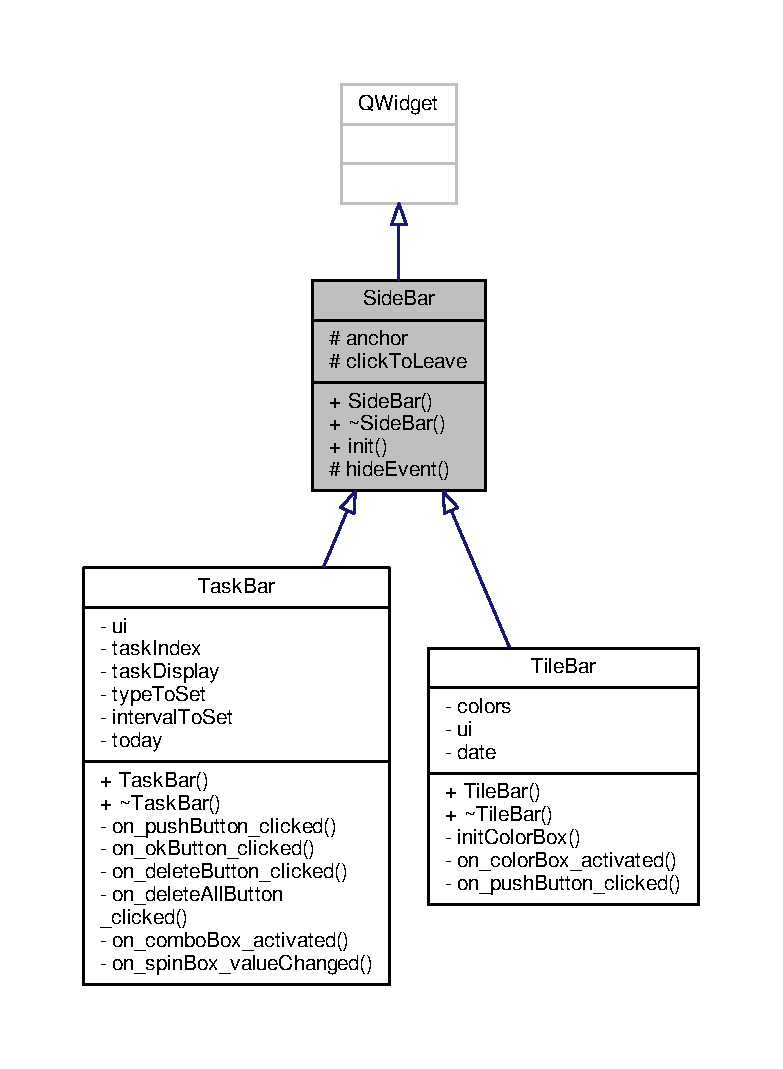
\includegraphics[width=350pt]{classSideBar__inherit__graph}
\end{center}
\end{figure}


Collaboration diagram for Side\+Bar\+:
\nopagebreak
\begin{figure}[H]
\begin{center}
\leavevmode
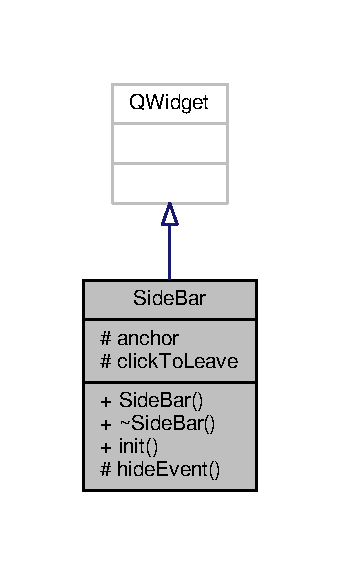
\includegraphics[width=163pt]{classSideBar__coll__graph}
\end{center}
\end{figure}
\subsection*{Public Member Functions}
\begin{DoxyCompactItemize}
\item 
\hyperlink{classSideBar_a9a331f6c3df3538c9cb8f5cb55f70aa6}{Side\+Bar} (Q\+Widget $\ast$\+\_\+anchor, bool \+\_\+click\+To\+Leave, Q\+Widget $\ast$parent=0)
\item 
\hyperlink{classSideBar_ab6585fb18d33836f7210a804eb9fcfa0}{$\sim$\+Side\+Bar} ()
\item 
void \hyperlink{classSideBar_af019dc58f6715e159a625a6628c2b126}{init} ()
\end{DoxyCompactItemize}
\subsection*{Protected Member Functions}
\begin{DoxyCompactItemize}
\item 
void \hyperlink{classSideBar_ac03ec8432ae5bc1849cbeade35f9458c}{hide\+Event} (Q\+Hide\+Event $\ast$event)
\end{DoxyCompactItemize}
\subsection*{Protected Attributes}
\begin{DoxyCompactItemize}
\item 
Q\+Widget $\ast$ \hyperlink{classSideBar_a0a6a0df257a08bdf785aeb155870efbc}{anchor}
\item 
bool \hyperlink{classSideBar_a8d0dba44a11de50893409620294498fb}{click\+To\+Leave}
\end{DoxyCompactItemize}


\subsection{Detailed Description}
Base class for side bar besides a day or a task. 

\subsection{Constructor \& Destructor Documentation}
\index{Side\+Bar@{Side\+Bar}!Side\+Bar@{Side\+Bar}}
\index{Side\+Bar@{Side\+Bar}!Side\+Bar@{Side\+Bar}}
\subsubsection[{\texorpdfstring{Side\+Bar(\+Q\+Widget $\ast$\+\_\+anchor, bool \+\_\+click\+To\+Leave, Q\+Widget $\ast$parent=0)}{SideBar(QWidget *_anchor, bool _clickToLeave, QWidget *parent=0)}}]{\setlength{\rightskip}{0pt plus 5cm}Side\+Bar\+::\+Side\+Bar (
\begin{DoxyParamCaption}
\item[{Q\+Widget $\ast$}]{\+\_\+anchor, }
\item[{bool}]{\+\_\+click\+To\+Leave, }
\item[{Q\+Widget $\ast$}]{parent = {\ttfamily 0}}
\end{DoxyParamCaption}
)\hspace{0.3cm}{\ttfamily [explicit]}}\hypertarget{classSideBar_a9a331f6c3df3538c9cb8f5cb55f70aa6}{}\label{classSideBar_a9a331f6c3df3538c9cb8f5cb55f70aa6}

\begin{DoxyParams}{Parameters}
{\em \+\_\+anchor} & \+: to show from which widget\textquotesingle{}s \\
\hline
{\em \+\_\+click\+To\+Leave} & \+: click anywhere outside to exit \\
\hline
\end{DoxyParams}
\index{Side\+Bar@{Side\+Bar}!````~Side\+Bar@{$\sim$\+Side\+Bar}}
\index{````~Side\+Bar@{$\sim$\+Side\+Bar}!Side\+Bar@{Side\+Bar}}
\subsubsection[{\texorpdfstring{$\sim$\+Side\+Bar()}{~SideBar()}}]{\setlength{\rightskip}{0pt plus 5cm}Side\+Bar\+::$\sim$\+Side\+Bar (
\begin{DoxyParamCaption}
{}
\end{DoxyParamCaption}
)}\hypertarget{classSideBar_ab6585fb18d33836f7210a804eb9fcfa0}{}\label{classSideBar_ab6585fb18d33836f7210a804eb9fcfa0}


\subsection{Member Function Documentation}
\index{Side\+Bar@{Side\+Bar}!hide\+Event@{hide\+Event}}
\index{hide\+Event@{hide\+Event}!Side\+Bar@{Side\+Bar}}
\subsubsection[{\texorpdfstring{hide\+Event(\+Q\+Hide\+Event $\ast$event)}{hideEvent(QHideEvent *event)}}]{\setlength{\rightskip}{0pt plus 5cm}void Side\+Bar\+::hide\+Event (
\begin{DoxyParamCaption}
\item[{Q\+Hide\+Event $\ast$}]{event}
\end{DoxyParamCaption}
)\hspace{0.3cm}{\ttfamily [protected]}}\hypertarget{classSideBar_ac03ec8432ae5bc1849cbeade35f9458c}{}\label{classSideBar_ac03ec8432ae5bc1849cbeade35f9458c}
\index{Side\+Bar@{Side\+Bar}!init@{init}}
\index{init@{init}!Side\+Bar@{Side\+Bar}}
\subsubsection[{\texorpdfstring{init()}{init()}}]{\setlength{\rightskip}{0pt plus 5cm}void Side\+Bar\+::init (
\begin{DoxyParamCaption}
{}
\end{DoxyParamCaption}
)}\hypertarget{classSideBar_af019dc58f6715e159a625a6628c2b126}{}\label{classSideBar_af019dc58f6715e159a625a6628c2b126}


\subsection{Member Data Documentation}
\index{Side\+Bar@{Side\+Bar}!anchor@{anchor}}
\index{anchor@{anchor}!Side\+Bar@{Side\+Bar}}
\subsubsection[{\texorpdfstring{anchor}{anchor}}]{\setlength{\rightskip}{0pt plus 5cm}Q\+Widget$\ast$ Side\+Bar\+::anchor\hspace{0.3cm}{\ttfamily [protected]}}\hypertarget{classSideBar_a0a6a0df257a08bdf785aeb155870efbc}{}\label{classSideBar_a0a6a0df257a08bdf785aeb155870efbc}
\index{Side\+Bar@{Side\+Bar}!click\+To\+Leave@{click\+To\+Leave}}
\index{click\+To\+Leave@{click\+To\+Leave}!Side\+Bar@{Side\+Bar}}
\subsubsection[{\texorpdfstring{click\+To\+Leave}{clickToLeave}}]{\setlength{\rightskip}{0pt plus 5cm}bool Side\+Bar\+::click\+To\+Leave\hspace{0.3cm}{\ttfamily [protected]}}\hypertarget{classSideBar_a8d0dba44a11de50893409620294498fb}{}\label{classSideBar_a8d0dba44a11de50893409620294498fb}


The documentation for this class was generated from the following files\+:\begin{DoxyCompactItemize}
\item 
\hyperlink{sidebar_8h}{sidebar.\+h}\item 
\hyperlink{sidebar_8cpp}{sidebar.\+cpp}\end{DoxyCompactItemize}

\hypertarget{classTask}{}\section{Task Class Reference}
\label{classTask}\index{Task@{Task}}


A task defined by user.  




{\ttfamily \#include $<$task.\+h$>$}



Inheritance diagram for Task\+:
\nopagebreak
\begin{figure}[H]
\begin{center}
\leavevmode
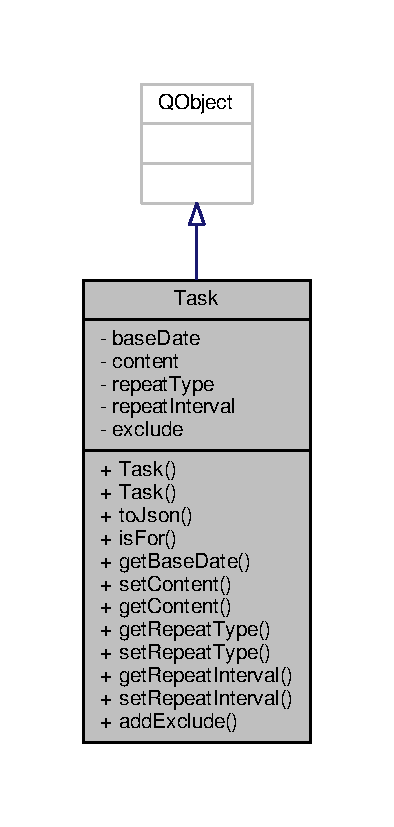
\includegraphics[width=189pt]{classTask__inherit__graph}
\end{center}
\end{figure}


Collaboration diagram for Task\+:
\nopagebreak
\begin{figure}[H]
\begin{center}
\leavevmode
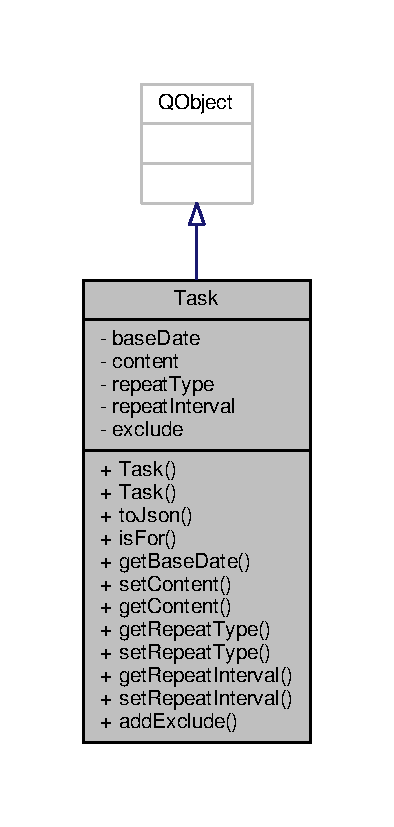
\includegraphics[width=189pt]{classTask__coll__graph}
\end{center}
\end{figure}
\subsection*{Public Types}
\begin{DoxyCompactItemize}
\item 
enum \hyperlink{classTask_a93fe2c7346381e2e631fb2ba63ac0344}{Repeat\+Type} \{ \hyperlink{classTask_a93fe2c7346381e2e631fb2ba63ac0344a1489a46f05a9ab3e7aa6f14871244839}{N\+O\+NE} = 0, 
\hyperlink{classTask_a93fe2c7346381e2e631fb2ba63ac0344a80a9ff87a14a3a59573514ed327e5d6f}{B\+Y\+\_\+\+D\+AY} = 1, 
\hyperlink{classTask_a93fe2c7346381e2e631fb2ba63ac0344a1a1cd5e7a9aad514a1b530284a3a23fc}{B\+Y\+\_\+\+M\+O\+N\+TH} = 2, 
\hyperlink{classTask_a93fe2c7346381e2e631fb2ba63ac0344acddd3dcd814b4580446ae57f75bf73e9}{B\+Y\+\_\+\+Y\+E\+AR} = 3
 \}
\end{DoxyCompactItemize}
\subsection*{Public Member Functions}
\begin{DoxyCompactItemize}
\item 
\hyperlink{classTask_a3d57c110575c95c1330081ed1b1b1027}{Task} (Q\+Json\+Value\+Ref json, Q\+Object $\ast$parent)
\begin{DoxyCompactList}\small\item\em Parse from json. \end{DoxyCompactList}\item 
\hyperlink{classTask_aaa27e6562bc6404bb23f138d0396e9a9}{Task} (const Q\+Date \&\+\_\+base\+Date, Q\+Object $\ast$parent)
\begin{DoxyCompactList}\small\item\em New task for a day. \end{DoxyCompactList}\item 
Q\+Json\+Value \hyperlink{classTask_a5ffa10b62035b2a6de0a7acf4dbe60a5}{to\+Json} () const 
\begin{DoxyCompactList}\small\item\em Output to json. \end{DoxyCompactList}\item 
bool \hyperlink{classTask_a506d5da7826ae91f3e51e4691f81083f}{is\+For} (const Q\+Date \&day) const 
\begin{DoxyCompactList}\small\item\em Check whether the task should be applied to a day. \end{DoxyCompactList}\item 
const Q\+Date \& \hyperlink{classTask_a03199e980185fd24a07442ea375fece0}{get\+Base\+Date} () const 
\item 
void \hyperlink{classTask_a10cfbaedd28879927a579e14740f4a40}{set\+Content} (const Q\+String \&\+\_\+content)
\item 
const Q\+String \& \hyperlink{classTask_af5ae0c97475e8d95864ad811042b3667}{get\+Content} () const 
\item 
\hyperlink{classTask_a93fe2c7346381e2e631fb2ba63ac0344}{Repeat\+Type} \hyperlink{classTask_aa824ffb74b452fd79d24e82722e1e125}{get\+Repeat\+Type} () const 
\item 
void \hyperlink{classTask_ac61ce4293a793137e050c04cf085d362}{set\+Repeat\+Type} (\hyperlink{classTask_a93fe2c7346381e2e631fb2ba63ac0344}{Repeat\+Type} t)
\item 
int \hyperlink{classTask_a39181e9cb138b93ebba4e5108e236f5e}{get\+Repeat\+Interval} () const 
\item 
void \hyperlink{classTask_a47e36fa7a3acff3d747d58fc4ce62217}{set\+Repeat\+Interval} (int interval)
\item 
void \hyperlink{classTask_a33ae4045c8be35cf12d60eba969a7e0e}{add\+Exclude} (const Q\+Date \&day)
\end{DoxyCompactItemize}
\subsection*{Private Attributes}
\begin{DoxyCompactItemize}
\item 
Q\+Date \hyperlink{classTask_a20cc2347b30cba60fb1da685ef8756c5}{base\+Date}
\item 
Q\+String \hyperlink{classTask_a9432e6a8bd681ddff95d3ee646193267}{content}
\item 
\hyperlink{classTask_a93fe2c7346381e2e631fb2ba63ac0344}{Repeat\+Type} \hyperlink{classTask_adf98bd28ce45d18bcc9f337cc425fd89}{repeat\+Type}
\item 
int \hyperlink{classTask_af61e693a3a2dec42646081d60c57df3e}{repeat\+Interval}
\item 
Q\+List$<$ Q\+Date $>$ \hyperlink{classTask_a7ea8d8cc5ad0786d7e1b0bbc34f58863}{exclude}
\end{DoxyCompactItemize}


\subsection{Detailed Description}
A task defined by user. 

\subsection{Member Enumeration Documentation}
\index{Task@{Task}!Repeat\+Type@{Repeat\+Type}}
\index{Repeat\+Type@{Repeat\+Type}!Task@{Task}}
\subsubsection[{\texorpdfstring{Repeat\+Type}{RepeatType}}]{\setlength{\rightskip}{0pt plus 5cm}enum {\bf Task\+::\+Repeat\+Type}}\hypertarget{classTask_a93fe2c7346381e2e631fb2ba63ac0344}{}\label{classTask_a93fe2c7346381e2e631fb2ba63ac0344}
\begin{Desc}
\item[Enumerator]\par
\begin{description}
\index{N\+O\+NE@{N\+O\+NE}!Task@{Task}}\index{Task@{Task}!N\+O\+NE@{N\+O\+NE}}\item[{\em 
N\+O\+NE\hypertarget{classTask_a93fe2c7346381e2e631fb2ba63ac0344a1489a46f05a9ab3e7aa6f14871244839}{}\label{classTask_a93fe2c7346381e2e631fb2ba63ac0344a1489a46f05a9ab3e7aa6f14871244839}
}]\index{B\+Y\+\_\+\+D\+AY@{B\+Y\+\_\+\+D\+AY}!Task@{Task}}\index{Task@{Task}!B\+Y\+\_\+\+D\+AY@{B\+Y\+\_\+\+D\+AY}}\item[{\em 
B\+Y\+\_\+\+D\+AY\hypertarget{classTask_a93fe2c7346381e2e631fb2ba63ac0344a80a9ff87a14a3a59573514ed327e5d6f}{}\label{classTask_a93fe2c7346381e2e631fb2ba63ac0344a80a9ff87a14a3a59573514ed327e5d6f}
}]\index{B\+Y\+\_\+\+M\+O\+N\+TH@{B\+Y\+\_\+\+M\+O\+N\+TH}!Task@{Task}}\index{Task@{Task}!B\+Y\+\_\+\+M\+O\+N\+TH@{B\+Y\+\_\+\+M\+O\+N\+TH}}\item[{\em 
B\+Y\+\_\+\+M\+O\+N\+TH\hypertarget{classTask_a93fe2c7346381e2e631fb2ba63ac0344a1a1cd5e7a9aad514a1b530284a3a23fc}{}\label{classTask_a93fe2c7346381e2e631fb2ba63ac0344a1a1cd5e7a9aad514a1b530284a3a23fc}
}]\index{B\+Y\+\_\+\+Y\+E\+AR@{B\+Y\+\_\+\+Y\+E\+AR}!Task@{Task}}\index{Task@{Task}!B\+Y\+\_\+\+Y\+E\+AR@{B\+Y\+\_\+\+Y\+E\+AR}}\item[{\em 
B\+Y\+\_\+\+Y\+E\+AR\hypertarget{classTask_a93fe2c7346381e2e631fb2ba63ac0344acddd3dcd814b4580446ae57f75bf73e9}{}\label{classTask_a93fe2c7346381e2e631fb2ba63ac0344acddd3dcd814b4580446ae57f75bf73e9}
}]\end{description}
\end{Desc}


\subsection{Constructor \& Destructor Documentation}
\index{Task@{Task}!Task@{Task}}
\index{Task@{Task}!Task@{Task}}
\subsubsection[{\texorpdfstring{Task(\+Q\+Json\+Value\+Ref json, Q\+Object $\ast$parent)}{Task(QJsonValueRef json, QObject *parent)}}]{\setlength{\rightskip}{0pt plus 5cm}Task\+::\+Task (
\begin{DoxyParamCaption}
\item[{Q\+Json\+Value\+Ref}]{json, }
\item[{Q\+Object $\ast$}]{parent}
\end{DoxyParamCaption}
)\hspace{0.3cm}{\ttfamily [explicit]}}\hypertarget{classTask_a3d57c110575c95c1330081ed1b1b1027}{}\label{classTask_a3d57c110575c95c1330081ed1b1b1027}


Parse from json. 

\index{Task@{Task}!Task@{Task}}
\index{Task@{Task}!Task@{Task}}
\subsubsection[{\texorpdfstring{Task(const Q\+Date \&\+\_\+base\+Date, Q\+Object $\ast$parent)}{Task(const QDate &_baseDate, QObject *parent)}}]{\setlength{\rightskip}{0pt plus 5cm}Task\+::\+Task (
\begin{DoxyParamCaption}
\item[{const Q\+Date \&}]{\+\_\+base\+Date, }
\item[{Q\+Object $\ast$}]{parent}
\end{DoxyParamCaption}
)\hspace{0.3cm}{\ttfamily [explicit]}}\hypertarget{classTask_aaa27e6562bc6404bb23f138d0396e9a9}{}\label{classTask_aaa27e6562bc6404bb23f138d0396e9a9}


New task for a day. 



\subsection{Member Function Documentation}
\index{Task@{Task}!add\+Exclude@{add\+Exclude}}
\index{add\+Exclude@{add\+Exclude}!Task@{Task}}
\subsubsection[{\texorpdfstring{add\+Exclude(const Q\+Date \&day)}{addExclude(const QDate &day)}}]{\setlength{\rightskip}{0pt plus 5cm}void Task\+::add\+Exclude (
\begin{DoxyParamCaption}
\item[{const Q\+Date \&}]{day}
\end{DoxyParamCaption}
)}\hypertarget{classTask_a33ae4045c8be35cf12d60eba969a7e0e}{}\label{classTask_a33ae4045c8be35cf12d60eba969a7e0e}
\index{Task@{Task}!get\+Base\+Date@{get\+Base\+Date}}
\index{get\+Base\+Date@{get\+Base\+Date}!Task@{Task}}
\subsubsection[{\texorpdfstring{get\+Base\+Date() const }{getBaseDate() const }}]{\setlength{\rightskip}{0pt plus 5cm}const Q\+Date \& Task\+::get\+Base\+Date (
\begin{DoxyParamCaption}
{}
\end{DoxyParamCaption}
) const}\hypertarget{classTask_a03199e980185fd24a07442ea375fece0}{}\label{classTask_a03199e980185fd24a07442ea375fece0}
\index{Task@{Task}!get\+Content@{get\+Content}}
\index{get\+Content@{get\+Content}!Task@{Task}}
\subsubsection[{\texorpdfstring{get\+Content() const }{getContent() const }}]{\setlength{\rightskip}{0pt plus 5cm}const Q\+String \& Task\+::get\+Content (
\begin{DoxyParamCaption}
{}
\end{DoxyParamCaption}
) const}\hypertarget{classTask_af5ae0c97475e8d95864ad811042b3667}{}\label{classTask_af5ae0c97475e8d95864ad811042b3667}
\index{Task@{Task}!get\+Repeat\+Interval@{get\+Repeat\+Interval}}
\index{get\+Repeat\+Interval@{get\+Repeat\+Interval}!Task@{Task}}
\subsubsection[{\texorpdfstring{get\+Repeat\+Interval() const }{getRepeatInterval() const }}]{\setlength{\rightskip}{0pt plus 5cm}int Task\+::get\+Repeat\+Interval (
\begin{DoxyParamCaption}
{}
\end{DoxyParamCaption}
) const}\hypertarget{classTask_a39181e9cb138b93ebba4e5108e236f5e}{}\label{classTask_a39181e9cb138b93ebba4e5108e236f5e}
\index{Task@{Task}!get\+Repeat\+Type@{get\+Repeat\+Type}}
\index{get\+Repeat\+Type@{get\+Repeat\+Type}!Task@{Task}}
\subsubsection[{\texorpdfstring{get\+Repeat\+Type() const }{getRepeatType() const }}]{\setlength{\rightskip}{0pt plus 5cm}{\bf Task\+::\+Repeat\+Type} Task\+::get\+Repeat\+Type (
\begin{DoxyParamCaption}
{}
\end{DoxyParamCaption}
) const}\hypertarget{classTask_aa824ffb74b452fd79d24e82722e1e125}{}\label{classTask_aa824ffb74b452fd79d24e82722e1e125}
\index{Task@{Task}!is\+For@{is\+For}}
\index{is\+For@{is\+For}!Task@{Task}}
\subsubsection[{\texorpdfstring{is\+For(const Q\+Date \&day) const }{isFor(const QDate &day) const }}]{\setlength{\rightskip}{0pt plus 5cm}bool Task\+::is\+For (
\begin{DoxyParamCaption}
\item[{const Q\+Date \&}]{day}
\end{DoxyParamCaption}
) const}\hypertarget{classTask_a506d5da7826ae91f3e51e4691f81083f}{}\label{classTask_a506d5da7826ae91f3e51e4691f81083f}


Check whether the task should be applied to a day. 

\index{Task@{Task}!set\+Content@{set\+Content}}
\index{set\+Content@{set\+Content}!Task@{Task}}
\subsubsection[{\texorpdfstring{set\+Content(const Q\+String \&\+\_\+content)}{setContent(const QString &_content)}}]{\setlength{\rightskip}{0pt plus 5cm}void Task\+::set\+Content (
\begin{DoxyParamCaption}
\item[{const Q\+String \&}]{\+\_\+content}
\end{DoxyParamCaption}
)}\hypertarget{classTask_a10cfbaedd28879927a579e14740f4a40}{}\label{classTask_a10cfbaedd28879927a579e14740f4a40}
\index{Task@{Task}!set\+Repeat\+Interval@{set\+Repeat\+Interval}}
\index{set\+Repeat\+Interval@{set\+Repeat\+Interval}!Task@{Task}}
\subsubsection[{\texorpdfstring{set\+Repeat\+Interval(int interval)}{setRepeatInterval(int interval)}}]{\setlength{\rightskip}{0pt plus 5cm}void Task\+::set\+Repeat\+Interval (
\begin{DoxyParamCaption}
\item[{int}]{interval}
\end{DoxyParamCaption}
)}\hypertarget{classTask_a47e36fa7a3acff3d747d58fc4ce62217}{}\label{classTask_a47e36fa7a3acff3d747d58fc4ce62217}
\index{Task@{Task}!set\+Repeat\+Type@{set\+Repeat\+Type}}
\index{set\+Repeat\+Type@{set\+Repeat\+Type}!Task@{Task}}
\subsubsection[{\texorpdfstring{set\+Repeat\+Type(\+Repeat\+Type t)}{setRepeatType(RepeatType t)}}]{\setlength{\rightskip}{0pt plus 5cm}void Task\+::set\+Repeat\+Type (
\begin{DoxyParamCaption}
\item[{{\bf Repeat\+Type}}]{t}
\end{DoxyParamCaption}
)}\hypertarget{classTask_ac61ce4293a793137e050c04cf085d362}{}\label{classTask_ac61ce4293a793137e050c04cf085d362}
\index{Task@{Task}!to\+Json@{to\+Json}}
\index{to\+Json@{to\+Json}!Task@{Task}}
\subsubsection[{\texorpdfstring{to\+Json() const }{toJson() const }}]{\setlength{\rightskip}{0pt plus 5cm}Q\+Json\+Value Task\+::to\+Json (
\begin{DoxyParamCaption}
{}
\end{DoxyParamCaption}
) const}\hypertarget{classTask_a5ffa10b62035b2a6de0a7acf4dbe60a5}{}\label{classTask_a5ffa10b62035b2a6de0a7acf4dbe60a5}


Output to json. 



\subsection{Member Data Documentation}
\index{Task@{Task}!base\+Date@{base\+Date}}
\index{base\+Date@{base\+Date}!Task@{Task}}
\subsubsection[{\texorpdfstring{base\+Date}{baseDate}}]{\setlength{\rightskip}{0pt plus 5cm}Q\+Date Task\+::base\+Date\hspace{0.3cm}{\ttfamily [private]}}\hypertarget{classTask_a20cc2347b30cba60fb1da685ef8756c5}{}\label{classTask_a20cc2347b30cba60fb1da685ef8756c5}
\index{Task@{Task}!content@{content}}
\index{content@{content}!Task@{Task}}
\subsubsection[{\texorpdfstring{content}{content}}]{\setlength{\rightskip}{0pt plus 5cm}Q\+String Task\+::content\hspace{0.3cm}{\ttfamily [private]}}\hypertarget{classTask_a9432e6a8bd681ddff95d3ee646193267}{}\label{classTask_a9432e6a8bd681ddff95d3ee646193267}
\index{Task@{Task}!exclude@{exclude}}
\index{exclude@{exclude}!Task@{Task}}
\subsubsection[{\texorpdfstring{exclude}{exclude}}]{\setlength{\rightskip}{0pt plus 5cm}Q\+List$<$Q\+Date$>$ Task\+::exclude\hspace{0.3cm}{\ttfamily [private]}}\hypertarget{classTask_a7ea8d8cc5ad0786d7e1b0bbc34f58863}{}\label{classTask_a7ea8d8cc5ad0786d7e1b0bbc34f58863}
\index{Task@{Task}!repeat\+Interval@{repeat\+Interval}}
\index{repeat\+Interval@{repeat\+Interval}!Task@{Task}}
\subsubsection[{\texorpdfstring{repeat\+Interval}{repeatInterval}}]{\setlength{\rightskip}{0pt plus 5cm}int Task\+::repeat\+Interval\hspace{0.3cm}{\ttfamily [private]}}\hypertarget{classTask_af61e693a3a2dec42646081d60c57df3e}{}\label{classTask_af61e693a3a2dec42646081d60c57df3e}
\index{Task@{Task}!repeat\+Type@{repeat\+Type}}
\index{repeat\+Type@{repeat\+Type}!Task@{Task}}
\subsubsection[{\texorpdfstring{repeat\+Type}{repeatType}}]{\setlength{\rightskip}{0pt plus 5cm}{\bf Repeat\+Type} Task\+::repeat\+Type\hspace{0.3cm}{\ttfamily [private]}}\hypertarget{classTask_adf98bd28ce45d18bcc9f337cc425fd89}{}\label{classTask_adf98bd28ce45d18bcc9f337cc425fd89}


The documentation for this class was generated from the following files\+:\begin{DoxyCompactItemize}
\item 
\hyperlink{task_8h}{task.\+h}\item 
\hyperlink{task_8cpp}{task.\+cpp}\end{DoxyCompactItemize}

\hypertarget{classTaskBar}{}\section{Task\+Bar Class Reference}
\label{classTaskBar}\index{Task\+Bar@{Task\+Bar}}


Provide an interface for users to interact with tasks.  




{\ttfamily \#include $<$taskbar.\+h$>$}



Inheritance diagram for Task\+Bar\+:
\nopagebreak
\begin{figure}[H]
\begin{center}
\leavevmode
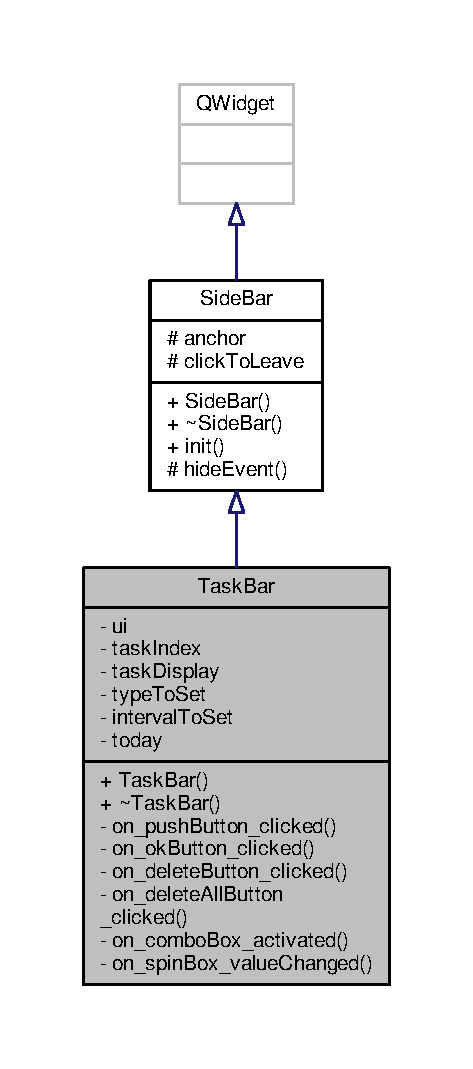
\includegraphics[width=227pt]{classTaskBar__inherit__graph}
\end{center}
\end{figure}


Collaboration diagram for Task\+Bar\+:
\nopagebreak
\begin{figure}[H]
\begin{center}
\leavevmode
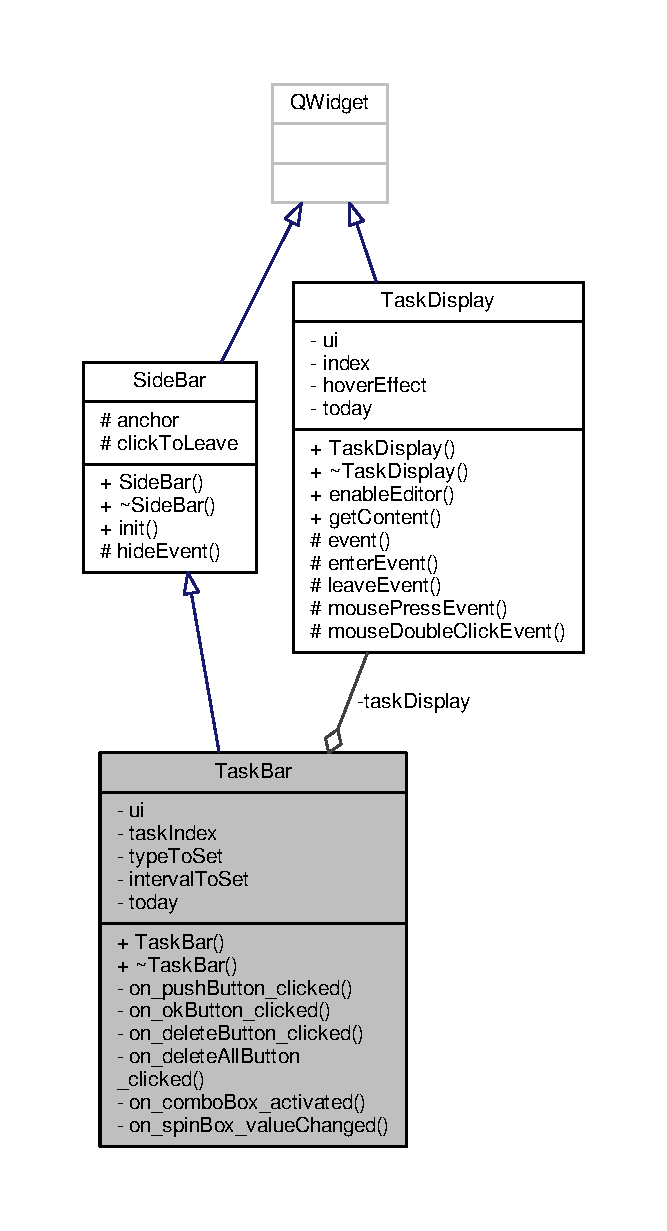
\includegraphics[height=550pt]{classTaskBar__coll__graph}
\end{center}
\end{figure}
\subsection*{Public Member Functions}
\begin{DoxyCompactItemize}
\item 
\hyperlink{classTaskBar_a62dbb456b9dd72f6e2c5f07e1765dbfe}{Task\+Bar} (Q\+Widget $\ast$\hyperlink{classSideBar_a0a6a0df257a08bdf785aeb155870efbc}{anchor}, int \+\_\+task\+Index, Q\+Date \+\_\+today, Q\+Widget $\ast$parent)
\item 
\hyperlink{classTaskBar_aba46bb3cba29968c2790a5ecfc2d3eba}{$\sim$\+Task\+Bar} ()
\end{DoxyCompactItemize}
\subsection*{Private Slots}
\begin{DoxyCompactItemize}
\item 
void \hyperlink{classTaskBar_acf2c1f19d61d67bb3c078c263042012a}{on\+\_\+push\+Button\+\_\+clicked} (bool checked)
\item 
void \hyperlink{classTaskBar_a2b2c67c68a830705af3c568b2e005d4d}{on\+\_\+ok\+Button\+\_\+clicked} (bool checked)
\item 
void \hyperlink{classTaskBar_adeb4b20f6055736acc7a042698c337ff}{on\+\_\+delete\+Button\+\_\+clicked} (bool checked)
\item 
void \hyperlink{classTaskBar_ab3127214b1aa8e3886f77b7b9c11f19e}{on\+\_\+delete\+All\+Button\+\_\+clicked} (bool checked)
\item 
void \hyperlink{classTaskBar_a10bf9a5d0649e13e395e04717c0b1490}{on\+\_\+combo\+Box\+\_\+activated} (int index)
\item 
void \hyperlink{classTaskBar_ab187953b1f39520cfb1b0792850bbfe8}{on\+\_\+spin\+Box\+\_\+value\+Changed} (int arg1)
\end{DoxyCompactItemize}
\subsection*{Private Attributes}
\begin{DoxyCompactItemize}
\item 
Ui\+::\+Task\+Bar $\ast$ \hyperlink{classTaskBar_adf231c032cb316cc500191fa349de0c8}{ui}
\item 
int \hyperlink{classTaskBar_a3207c8756b34796b9670f7cdc90bd121}{task\+Index}
\item 
\hyperlink{classTaskDisplay}{Task\+Display} $\ast$ \hyperlink{classTaskBar_ad0eb90c40336ebb502c31c8389c38bf0}{task\+Display}
\item 
\hyperlink{classTask_a93fe2c7346381e2e631fb2ba63ac0344}{Task\+::\+Repeat\+Type} \hyperlink{classTaskBar_a84684467e8038096bee94cdd1f26180c}{type\+To\+Set}
\begin{DoxyCompactList}\small\item\em to be set after clicking save \end{DoxyCompactList}\item 
int \hyperlink{classTaskBar_a4eb8a4530ebcb300192bb41013a91a1c}{interval\+To\+Set}
\item 
Q\+Date \hyperlink{classTaskBar_ab2cdbd96df84313d9de6e86fd968e374}{today}
\end{DoxyCompactItemize}
\subsection*{Additional Inherited Members}


\subsection{Detailed Description}
Provide an interface for users to interact with tasks. 

\subsection{Constructor \& Destructor Documentation}
\index{Task\+Bar@{Task\+Bar}!Task\+Bar@{Task\+Bar}}
\index{Task\+Bar@{Task\+Bar}!Task\+Bar@{Task\+Bar}}
\subsubsection[{\texorpdfstring{Task\+Bar(\+Q\+Widget $\ast$anchor, int \+\_\+task\+Index, Q\+Date \+\_\+today, Q\+Widget $\ast$parent)}{TaskBar(QWidget *anchor, int _taskIndex, QDate _today, QWidget *parent)}}]{\setlength{\rightskip}{0pt plus 5cm}Task\+Bar\+::\+Task\+Bar (
\begin{DoxyParamCaption}
\item[{Q\+Widget $\ast$}]{anchor, }
\item[{int}]{\+\_\+task\+Index, }
\item[{Q\+Date}]{\+\_\+today, }
\item[{Q\+Widget $\ast$}]{parent}
\end{DoxyParamCaption}
)\hspace{0.3cm}{\ttfamily [explicit]}}\hypertarget{classTaskBar_a62dbb456b9dd72f6e2c5f07e1765dbfe}{}\label{classTaskBar_a62dbb456b9dd72f6e2c5f07e1765dbfe}
\index{Task\+Bar@{Task\+Bar}!````~Task\+Bar@{$\sim$\+Task\+Bar}}
\index{````~Task\+Bar@{$\sim$\+Task\+Bar}!Task\+Bar@{Task\+Bar}}
\subsubsection[{\texorpdfstring{$\sim$\+Task\+Bar()}{~TaskBar()}}]{\setlength{\rightskip}{0pt plus 5cm}Task\+Bar\+::$\sim$\+Task\+Bar (
\begin{DoxyParamCaption}
{}
\end{DoxyParamCaption}
)}\hypertarget{classTaskBar_aba46bb3cba29968c2790a5ecfc2d3eba}{}\label{classTaskBar_aba46bb3cba29968c2790a5ecfc2d3eba}


\subsection{Member Function Documentation}
\index{Task\+Bar@{Task\+Bar}!on\+\_\+combo\+Box\+\_\+activated@{on\+\_\+combo\+Box\+\_\+activated}}
\index{on\+\_\+combo\+Box\+\_\+activated@{on\+\_\+combo\+Box\+\_\+activated}!Task\+Bar@{Task\+Bar}}
\subsubsection[{\texorpdfstring{on\+\_\+combo\+Box\+\_\+activated}{on_comboBox_activated}}]{\setlength{\rightskip}{0pt plus 5cm}void Task\+Bar\+::on\+\_\+combo\+Box\+\_\+activated (
\begin{DoxyParamCaption}
\item[{int}]{index}
\end{DoxyParamCaption}
)\hspace{0.3cm}{\ttfamily [private]}, {\ttfamily [slot]}}\hypertarget{classTaskBar_a10bf9a5d0649e13e395e04717c0b1490}{}\label{classTaskBar_a10bf9a5d0649e13e395e04717c0b1490}
\index{Task\+Bar@{Task\+Bar}!on\+\_\+delete\+All\+Button\+\_\+clicked@{on\+\_\+delete\+All\+Button\+\_\+clicked}}
\index{on\+\_\+delete\+All\+Button\+\_\+clicked@{on\+\_\+delete\+All\+Button\+\_\+clicked}!Task\+Bar@{Task\+Bar}}
\subsubsection[{\texorpdfstring{on\+\_\+delete\+All\+Button\+\_\+clicked}{on_deleteAllButton_clicked}}]{\setlength{\rightskip}{0pt plus 5cm}void Task\+Bar\+::on\+\_\+delete\+All\+Button\+\_\+clicked (
\begin{DoxyParamCaption}
\item[{bool}]{checked}
\end{DoxyParamCaption}
)\hspace{0.3cm}{\ttfamily [private]}, {\ttfamily [slot]}}\hypertarget{classTaskBar_ab3127214b1aa8e3886f77b7b9c11f19e}{}\label{classTaskBar_ab3127214b1aa8e3886f77b7b9c11f19e}
\index{Task\+Bar@{Task\+Bar}!on\+\_\+delete\+Button\+\_\+clicked@{on\+\_\+delete\+Button\+\_\+clicked}}
\index{on\+\_\+delete\+Button\+\_\+clicked@{on\+\_\+delete\+Button\+\_\+clicked}!Task\+Bar@{Task\+Bar}}
\subsubsection[{\texorpdfstring{on\+\_\+delete\+Button\+\_\+clicked}{on_deleteButton_clicked}}]{\setlength{\rightskip}{0pt plus 5cm}void Task\+Bar\+::on\+\_\+delete\+Button\+\_\+clicked (
\begin{DoxyParamCaption}
\item[{bool}]{checked}
\end{DoxyParamCaption}
)\hspace{0.3cm}{\ttfamily [private]}, {\ttfamily [slot]}}\hypertarget{classTaskBar_adeb4b20f6055736acc7a042698c337ff}{}\label{classTaskBar_adeb4b20f6055736acc7a042698c337ff}
\index{Task\+Bar@{Task\+Bar}!on\+\_\+ok\+Button\+\_\+clicked@{on\+\_\+ok\+Button\+\_\+clicked}}
\index{on\+\_\+ok\+Button\+\_\+clicked@{on\+\_\+ok\+Button\+\_\+clicked}!Task\+Bar@{Task\+Bar}}
\subsubsection[{\texorpdfstring{on\+\_\+ok\+Button\+\_\+clicked}{on_okButton_clicked}}]{\setlength{\rightskip}{0pt plus 5cm}void Task\+Bar\+::on\+\_\+ok\+Button\+\_\+clicked (
\begin{DoxyParamCaption}
\item[{bool}]{checked}
\end{DoxyParamCaption}
)\hspace{0.3cm}{\ttfamily [private]}, {\ttfamily [slot]}}\hypertarget{classTaskBar_a2b2c67c68a830705af3c568b2e005d4d}{}\label{classTaskBar_a2b2c67c68a830705af3c568b2e005d4d}
\index{Task\+Bar@{Task\+Bar}!on\+\_\+push\+Button\+\_\+clicked@{on\+\_\+push\+Button\+\_\+clicked}}
\index{on\+\_\+push\+Button\+\_\+clicked@{on\+\_\+push\+Button\+\_\+clicked}!Task\+Bar@{Task\+Bar}}
\subsubsection[{\texorpdfstring{on\+\_\+push\+Button\+\_\+clicked}{on_pushButton_clicked}}]{\setlength{\rightskip}{0pt plus 5cm}void Task\+Bar\+::on\+\_\+push\+Button\+\_\+clicked (
\begin{DoxyParamCaption}
\item[{bool}]{checked}
\end{DoxyParamCaption}
)\hspace{0.3cm}{\ttfamily [private]}, {\ttfamily [slot]}}\hypertarget{classTaskBar_acf2c1f19d61d67bb3c078c263042012a}{}\label{classTaskBar_acf2c1f19d61d67bb3c078c263042012a}
\index{Task\+Bar@{Task\+Bar}!on\+\_\+spin\+Box\+\_\+value\+Changed@{on\+\_\+spin\+Box\+\_\+value\+Changed}}
\index{on\+\_\+spin\+Box\+\_\+value\+Changed@{on\+\_\+spin\+Box\+\_\+value\+Changed}!Task\+Bar@{Task\+Bar}}
\subsubsection[{\texorpdfstring{on\+\_\+spin\+Box\+\_\+value\+Changed}{on_spinBox_valueChanged}}]{\setlength{\rightskip}{0pt plus 5cm}void Task\+Bar\+::on\+\_\+spin\+Box\+\_\+value\+Changed (
\begin{DoxyParamCaption}
\item[{int}]{arg1}
\end{DoxyParamCaption}
)\hspace{0.3cm}{\ttfamily [private]}, {\ttfamily [slot]}}\hypertarget{classTaskBar_ab187953b1f39520cfb1b0792850bbfe8}{}\label{classTaskBar_ab187953b1f39520cfb1b0792850bbfe8}


\subsection{Member Data Documentation}
\index{Task\+Bar@{Task\+Bar}!interval\+To\+Set@{interval\+To\+Set}}
\index{interval\+To\+Set@{interval\+To\+Set}!Task\+Bar@{Task\+Bar}}
\subsubsection[{\texorpdfstring{interval\+To\+Set}{intervalToSet}}]{\setlength{\rightskip}{0pt plus 5cm}int Task\+Bar\+::interval\+To\+Set\hspace{0.3cm}{\ttfamily [private]}}\hypertarget{classTaskBar_a4eb8a4530ebcb300192bb41013a91a1c}{}\label{classTaskBar_a4eb8a4530ebcb300192bb41013a91a1c}
\index{Task\+Bar@{Task\+Bar}!task\+Display@{task\+Display}}
\index{task\+Display@{task\+Display}!Task\+Bar@{Task\+Bar}}
\subsubsection[{\texorpdfstring{task\+Display}{taskDisplay}}]{\setlength{\rightskip}{0pt plus 5cm}{\bf Task\+Display}$\ast$ Task\+Bar\+::task\+Display\hspace{0.3cm}{\ttfamily [private]}}\hypertarget{classTaskBar_ad0eb90c40336ebb502c31c8389c38bf0}{}\label{classTaskBar_ad0eb90c40336ebb502c31c8389c38bf0}
\index{Task\+Bar@{Task\+Bar}!task\+Index@{task\+Index}}
\index{task\+Index@{task\+Index}!Task\+Bar@{Task\+Bar}}
\subsubsection[{\texorpdfstring{task\+Index}{taskIndex}}]{\setlength{\rightskip}{0pt plus 5cm}int Task\+Bar\+::task\+Index\hspace{0.3cm}{\ttfamily [private]}}\hypertarget{classTaskBar_a3207c8756b34796b9670f7cdc90bd121}{}\label{classTaskBar_a3207c8756b34796b9670f7cdc90bd121}
\index{Task\+Bar@{Task\+Bar}!today@{today}}
\index{today@{today}!Task\+Bar@{Task\+Bar}}
\subsubsection[{\texorpdfstring{today}{today}}]{\setlength{\rightskip}{0pt plus 5cm}Q\+Date Task\+Bar\+::today\hspace{0.3cm}{\ttfamily [private]}}\hypertarget{classTaskBar_ab2cdbd96df84313d9de6e86fd968e374}{}\label{classTaskBar_ab2cdbd96df84313d9de6e86fd968e374}
\index{Task\+Bar@{Task\+Bar}!type\+To\+Set@{type\+To\+Set}}
\index{type\+To\+Set@{type\+To\+Set}!Task\+Bar@{Task\+Bar}}
\subsubsection[{\texorpdfstring{type\+To\+Set}{typeToSet}}]{\setlength{\rightskip}{0pt plus 5cm}{\bf Task\+::\+Repeat\+Type} Task\+Bar\+::type\+To\+Set\hspace{0.3cm}{\ttfamily [private]}}\hypertarget{classTaskBar_a84684467e8038096bee94cdd1f26180c}{}\label{classTaskBar_a84684467e8038096bee94cdd1f26180c}


to be set after clicking save 

\index{Task\+Bar@{Task\+Bar}!ui@{ui}}
\index{ui@{ui}!Task\+Bar@{Task\+Bar}}
\subsubsection[{\texorpdfstring{ui}{ui}}]{\setlength{\rightskip}{0pt plus 5cm}Ui\+::\+Task\+Bar$\ast$ Task\+Bar\+::ui\hspace{0.3cm}{\ttfamily [private]}}\hypertarget{classTaskBar_adf231c032cb316cc500191fa349de0c8}{}\label{classTaskBar_adf231c032cb316cc500191fa349de0c8}


The documentation for this class was generated from the following files\+:\begin{DoxyCompactItemize}
\item 
\hyperlink{taskbar_8h}{taskbar.\+h}\item 
\hyperlink{taskbar_8cpp}{taskbar.\+cpp}\end{DoxyCompactItemize}

\hypertarget{classTaskDisplay}{}\section{Task\+Display Class Reference}
\label{classTaskDisplay}\index{Task\+Display@{Task\+Display}}


Display and edit a task.  




{\ttfamily \#include $<$taskdisplay.\+h$>$}



Inheritance diagram for Task\+Display\+:
\nopagebreak
\begin{figure}[H]
\begin{center}
\leavevmode
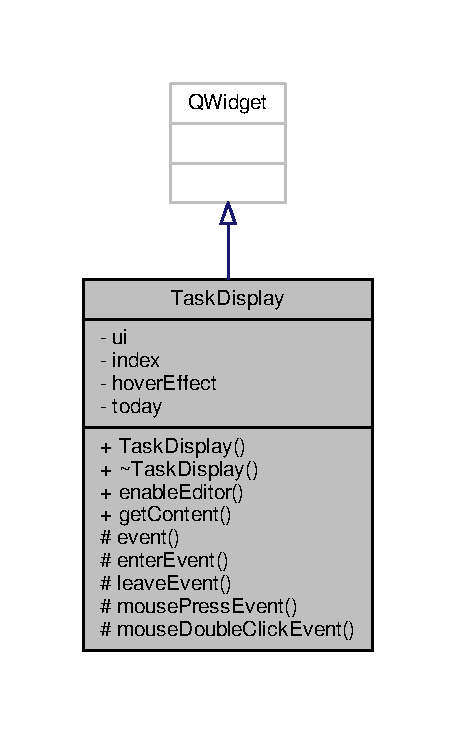
\includegraphics[width=219pt]{classTaskDisplay__inherit__graph}
\end{center}
\end{figure}


Collaboration diagram for Task\+Display\+:
\nopagebreak
\begin{figure}[H]
\begin{center}
\leavevmode
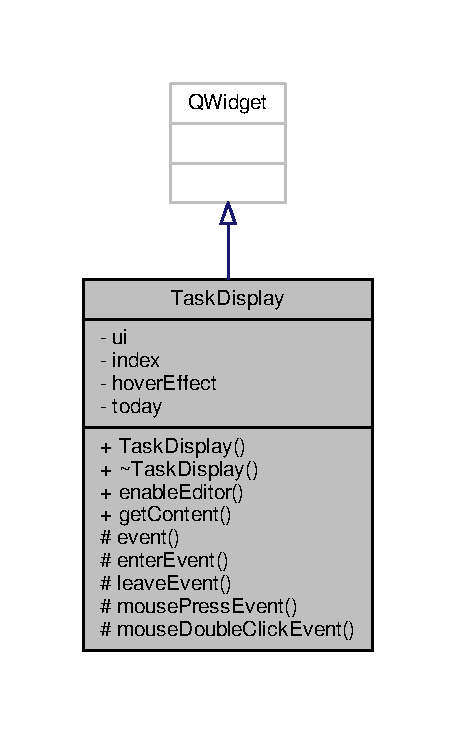
\includegraphics[width=219pt]{classTaskDisplay__coll__graph}
\end{center}
\end{figure}
\subsection*{Signals}
\begin{DoxyCompactItemize}
\item 
void \hyperlink{classTaskDisplay_a25d79a4505fb588372786e1798c826a7}{on\+Selected} (Q\+Widget $\ast$anchor, int task\+Index, Q\+Date \hyperlink{classTaskDisplay_a1adb50384f7db484b7f35c8952395157}{today})
\end{DoxyCompactItemize}
\subsection*{Public Member Functions}
\begin{DoxyCompactItemize}
\item 
\hyperlink{classTaskDisplay_acbfb32482b03fc1c64bf8658403f2af9}{Task\+Display} (int \+\_\+index, bool \+\_\+hover\+Effect, Q\+Date \+\_\+today, Q\+Widget $\ast$parent)
\item 
\hyperlink{classTaskDisplay_a5ce3c02b7a2d887b0842d5ae141a212e}{$\sim$\+Task\+Display} ()
\item 
void \hyperlink{classTaskDisplay_ae31dc04c0368ab8202067aec2751e2db}{enable\+Editor} ()
\item 
Q\+String \hyperlink{classTaskDisplay_a4d808c7da0c5c7c95d049a013b988fec}{get\+Content} () const 
\begin{DoxyCompactList}\small\item\em Get content in the editor. \end{DoxyCompactList}\end{DoxyCompactItemize}
\subsection*{Protected Member Functions}
\begin{DoxyCompactItemize}
\item 
bool \hyperlink{classTaskDisplay_a32caa0a9768c26e08864a46fe128ed74}{event} (Q\+Event $\ast$event)
\item 
void \hyperlink{classTaskDisplay_a6c59096df7c96c3bd3dfbc79df9a5712}{enter\+Event} (Q\+Event $\ast$\hyperlink{classTaskDisplay_a32caa0a9768c26e08864a46fe128ed74}{event})
\item 
void \hyperlink{classTaskDisplay_ac88db0d1766d9eb4b622cbfeb701fcc7}{leave\+Event} (Q\+Event $\ast$\hyperlink{classTaskDisplay_a32caa0a9768c26e08864a46fe128ed74}{event})
\item 
void \hyperlink{classTaskDisplay_a6c488759b6e70862f2138aa55262aaaf}{mouse\+Press\+Event} (Q\+Mouse\+Event $\ast$\hyperlink{classTaskDisplay_a32caa0a9768c26e08864a46fe128ed74}{event})
\item 
void \hyperlink{classTaskDisplay_a5c604068075246ce7f60d6e6432da284}{mouse\+Double\+Click\+Event} (Q\+Mouse\+Event $\ast$\hyperlink{classTaskDisplay_a32caa0a9768c26e08864a46fe128ed74}{event})
\end{DoxyCompactItemize}
\subsection*{Private Attributes}
\begin{DoxyCompactItemize}
\item 
Ui\+::\+Task\+Display $\ast$ \hyperlink{classTaskDisplay_a580ecd014e47a399bf6416fa31aff7da}{ui}
\item 
int \hyperlink{classTaskDisplay_a59c27396e432f0d65d4988aa917edb28}{index}
\item 
bool \hyperlink{classTaskDisplay_a1dcd9193b35d30e1321515e7d9aded08}{hover\+Effect}
\item 
Q\+Date \hyperlink{classTaskDisplay_a1adb50384f7db484b7f35c8952395157}{today}
\end{DoxyCompactItemize}


\subsection{Detailed Description}
Display and edit a task. 

\subsection{Constructor \& Destructor Documentation}
\index{Task\+Display@{Task\+Display}!Task\+Display@{Task\+Display}}
\index{Task\+Display@{Task\+Display}!Task\+Display@{Task\+Display}}
\subsubsection[{\texorpdfstring{Task\+Display(int \+\_\+index, bool \+\_\+hover\+Effect, Q\+Date \+\_\+today, Q\+Widget $\ast$parent)}{TaskDisplay(int _index, bool _hoverEffect, QDate _today, QWidget *parent)}}]{\setlength{\rightskip}{0pt plus 5cm}Task\+Display\+::\+Task\+Display (
\begin{DoxyParamCaption}
\item[{int}]{\+\_\+index, }
\item[{bool}]{\+\_\+hover\+Effect, }
\item[{Q\+Date}]{\+\_\+today, }
\item[{Q\+Widget $\ast$}]{parent}
\end{DoxyParamCaption}
)\hspace{0.3cm}{\ttfamily [explicit]}}\hypertarget{classTaskDisplay_acbfb32482b03fc1c64bf8658403f2af9}{}\label{classTaskDisplay_acbfb32482b03fc1c64bf8658403f2af9}

\begin{DoxyParams}{Parameters}
{\em \+\_\+index} & \+: task index \\
\hline
{\em \+\_\+hover\+Effect} & \+: whether to highlight on hover event and recieve double-\/click to prompt menu \\
\hline
\end{DoxyParams}
\index{Task\+Display@{Task\+Display}!````~Task\+Display@{$\sim$\+Task\+Display}}
\index{````~Task\+Display@{$\sim$\+Task\+Display}!Task\+Display@{Task\+Display}}
\subsubsection[{\texorpdfstring{$\sim$\+Task\+Display()}{~TaskDisplay()}}]{\setlength{\rightskip}{0pt plus 5cm}Task\+Display\+::$\sim$\+Task\+Display (
\begin{DoxyParamCaption}
{}
\end{DoxyParamCaption}
)}\hypertarget{classTaskDisplay_a5ce3c02b7a2d887b0842d5ae141a212e}{}\label{classTaskDisplay_a5ce3c02b7a2d887b0842d5ae141a212e}


\subsection{Member Function Documentation}
\index{Task\+Display@{Task\+Display}!enable\+Editor@{enable\+Editor}}
\index{enable\+Editor@{enable\+Editor}!Task\+Display@{Task\+Display}}
\subsubsection[{\texorpdfstring{enable\+Editor()}{enableEditor()}}]{\setlength{\rightskip}{0pt plus 5cm}void Task\+Display\+::enable\+Editor (
\begin{DoxyParamCaption}
{}
\end{DoxyParamCaption}
)}\hypertarget{classTaskDisplay_ae31dc04c0368ab8202067aec2751e2db}{}\label{classTaskDisplay_ae31dc04c0368ab8202067aec2751e2db}
\index{Task\+Display@{Task\+Display}!enter\+Event@{enter\+Event}}
\index{enter\+Event@{enter\+Event}!Task\+Display@{Task\+Display}}
\subsubsection[{\texorpdfstring{enter\+Event(\+Q\+Event $\ast$event)}{enterEvent(QEvent *event)}}]{\setlength{\rightskip}{0pt plus 5cm}void Task\+Display\+::enter\+Event (
\begin{DoxyParamCaption}
\item[{Q\+Event $\ast$}]{event}
\end{DoxyParamCaption}
)\hspace{0.3cm}{\ttfamily [protected]}}\hypertarget{classTaskDisplay_a6c59096df7c96c3bd3dfbc79df9a5712}{}\label{classTaskDisplay_a6c59096df7c96c3bd3dfbc79df9a5712}
\index{Task\+Display@{Task\+Display}!event@{event}}
\index{event@{event}!Task\+Display@{Task\+Display}}
\subsubsection[{\texorpdfstring{event(\+Q\+Event $\ast$event)}{event(QEvent *event)}}]{\setlength{\rightskip}{0pt plus 5cm}bool Task\+Display\+::event (
\begin{DoxyParamCaption}
\item[{Q\+Event $\ast$}]{event}
\end{DoxyParamCaption}
)\hspace{0.3cm}{\ttfamily [protected]}}\hypertarget{classTaskDisplay_a32caa0a9768c26e08864a46fe128ed74}{}\label{classTaskDisplay_a32caa0a9768c26e08864a46fe128ed74}
\index{Task\+Display@{Task\+Display}!get\+Content@{get\+Content}}
\index{get\+Content@{get\+Content}!Task\+Display@{Task\+Display}}
\subsubsection[{\texorpdfstring{get\+Content() const }{getContent() const }}]{\setlength{\rightskip}{0pt plus 5cm}Q\+String Task\+Display\+::get\+Content (
\begin{DoxyParamCaption}
{}
\end{DoxyParamCaption}
) const}\hypertarget{classTaskDisplay_a4d808c7da0c5c7c95d049a013b988fec}{}\label{classTaskDisplay_a4d808c7da0c5c7c95d049a013b988fec}


Get content in the editor. 

\index{Task\+Display@{Task\+Display}!leave\+Event@{leave\+Event}}
\index{leave\+Event@{leave\+Event}!Task\+Display@{Task\+Display}}
\subsubsection[{\texorpdfstring{leave\+Event(\+Q\+Event $\ast$event)}{leaveEvent(QEvent *event)}}]{\setlength{\rightskip}{0pt plus 5cm}void Task\+Display\+::leave\+Event (
\begin{DoxyParamCaption}
\item[{Q\+Event $\ast$}]{event}
\end{DoxyParamCaption}
)\hspace{0.3cm}{\ttfamily [protected]}}\hypertarget{classTaskDisplay_ac88db0d1766d9eb4b622cbfeb701fcc7}{}\label{classTaskDisplay_ac88db0d1766d9eb4b622cbfeb701fcc7}
\index{Task\+Display@{Task\+Display}!mouse\+Double\+Click\+Event@{mouse\+Double\+Click\+Event}}
\index{mouse\+Double\+Click\+Event@{mouse\+Double\+Click\+Event}!Task\+Display@{Task\+Display}}
\subsubsection[{\texorpdfstring{mouse\+Double\+Click\+Event(\+Q\+Mouse\+Event $\ast$event)}{mouseDoubleClickEvent(QMouseEvent *event)}}]{\setlength{\rightskip}{0pt plus 5cm}void Task\+Display\+::mouse\+Double\+Click\+Event (
\begin{DoxyParamCaption}
\item[{Q\+Mouse\+Event $\ast$}]{event}
\end{DoxyParamCaption}
)\hspace{0.3cm}{\ttfamily [protected]}}\hypertarget{classTaskDisplay_a5c604068075246ce7f60d6e6432da284}{}\label{classTaskDisplay_a5c604068075246ce7f60d6e6432da284}
\index{Task\+Display@{Task\+Display}!mouse\+Press\+Event@{mouse\+Press\+Event}}
\index{mouse\+Press\+Event@{mouse\+Press\+Event}!Task\+Display@{Task\+Display}}
\subsubsection[{\texorpdfstring{mouse\+Press\+Event(\+Q\+Mouse\+Event $\ast$event)}{mousePressEvent(QMouseEvent *event)}}]{\setlength{\rightskip}{0pt plus 5cm}void Task\+Display\+::mouse\+Press\+Event (
\begin{DoxyParamCaption}
\item[{Q\+Mouse\+Event $\ast$}]{event}
\end{DoxyParamCaption}
)\hspace{0.3cm}{\ttfamily [protected]}}\hypertarget{classTaskDisplay_a6c488759b6e70862f2138aa55262aaaf}{}\label{classTaskDisplay_a6c488759b6e70862f2138aa55262aaaf}
\index{Task\+Display@{Task\+Display}!on\+Selected@{on\+Selected}}
\index{on\+Selected@{on\+Selected}!Task\+Display@{Task\+Display}}
\subsubsection[{\texorpdfstring{on\+Selected}{onSelected}}]{\setlength{\rightskip}{0pt plus 5cm}void Task\+Display\+::on\+Selected (
\begin{DoxyParamCaption}
\item[{Q\+Widget $\ast$}]{anchor, }
\item[{int}]{task\+Index, }
\item[{Q\+Date}]{today}
\end{DoxyParamCaption}
)\hspace{0.3cm}{\ttfamily [signal]}}\hypertarget{classTaskDisplay_a25d79a4505fb588372786e1798c826a7}{}\label{classTaskDisplay_a25d79a4505fb588372786e1798c826a7}


\subsection{Member Data Documentation}
\index{Task\+Display@{Task\+Display}!hover\+Effect@{hover\+Effect}}
\index{hover\+Effect@{hover\+Effect}!Task\+Display@{Task\+Display}}
\subsubsection[{\texorpdfstring{hover\+Effect}{hoverEffect}}]{\setlength{\rightskip}{0pt plus 5cm}bool Task\+Display\+::hover\+Effect\hspace{0.3cm}{\ttfamily [private]}}\hypertarget{classTaskDisplay_a1dcd9193b35d30e1321515e7d9aded08}{}\label{classTaskDisplay_a1dcd9193b35d30e1321515e7d9aded08}
\index{Task\+Display@{Task\+Display}!index@{index}}
\index{index@{index}!Task\+Display@{Task\+Display}}
\subsubsection[{\texorpdfstring{index}{index}}]{\setlength{\rightskip}{0pt plus 5cm}int Task\+Display\+::index\hspace{0.3cm}{\ttfamily [private]}}\hypertarget{classTaskDisplay_a59c27396e432f0d65d4988aa917edb28}{}\label{classTaskDisplay_a59c27396e432f0d65d4988aa917edb28}
\index{Task\+Display@{Task\+Display}!today@{today}}
\index{today@{today}!Task\+Display@{Task\+Display}}
\subsubsection[{\texorpdfstring{today}{today}}]{\setlength{\rightskip}{0pt plus 5cm}Q\+Date Task\+Display\+::today\hspace{0.3cm}{\ttfamily [private]}}\hypertarget{classTaskDisplay_a1adb50384f7db484b7f35c8952395157}{}\label{classTaskDisplay_a1adb50384f7db484b7f35c8952395157}
\index{Task\+Display@{Task\+Display}!ui@{ui}}
\index{ui@{ui}!Task\+Display@{Task\+Display}}
\subsubsection[{\texorpdfstring{ui}{ui}}]{\setlength{\rightskip}{0pt plus 5cm}Ui\+::\+Task\+Display$\ast$ Task\+Display\+::ui\hspace{0.3cm}{\ttfamily [private]}}\hypertarget{classTaskDisplay_a580ecd014e47a399bf6416fa31aff7da}{}\label{classTaskDisplay_a580ecd014e47a399bf6416fa31aff7da}


The documentation for this class was generated from the following files\+:\begin{DoxyCompactItemize}
\item 
\hyperlink{taskdisplay_8h}{taskdisplay.\+h}\item 
\hyperlink{taskdisplay_8cpp}{taskdisplay.\+cpp}\end{DoxyCompactItemize}

\hypertarget{classTile}{}\section{Tile Class Reference}
\label{classTile}\index{Tile@{Tile}}


A grid cell response for a day.  




{\ttfamily \#include $<$tile.\+h$>$}



Inheritance diagram for Tile\+:
\nopagebreak
\begin{figure}[H]
\begin{center}
\leavevmode
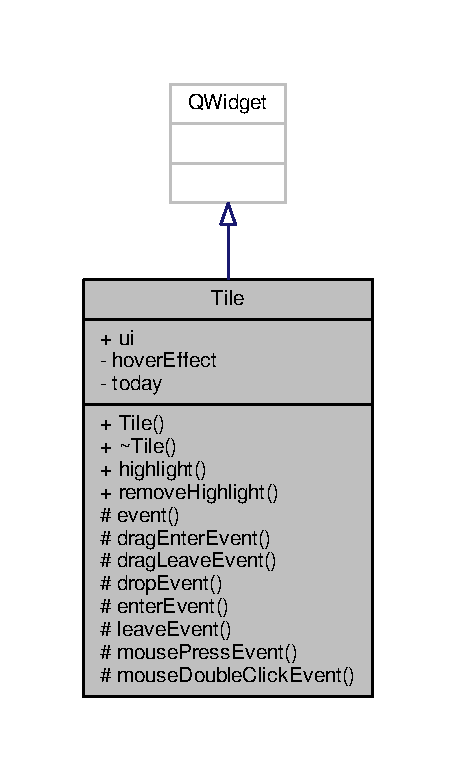
\includegraphics[width=219pt]{classTile__inherit__graph}
\end{center}
\end{figure}


Collaboration diagram for Tile\+:
\nopagebreak
\begin{figure}[H]
\begin{center}
\leavevmode
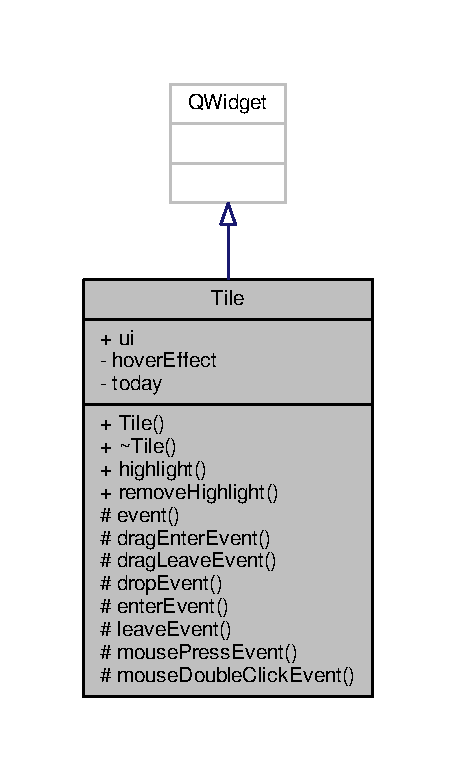
\includegraphics[width=219pt]{classTile__coll__graph}
\end{center}
\end{figure}
\subsection*{Signals}
\begin{DoxyCompactItemize}
\item 
void \hyperlink{classTile_a9df630a2ee5dc988f935f3eec20c71f1}{on\+Selected} ()
\begin{DoxyCompactList}\small\item\em Emitted when the tile is selected by double clicking. \end{DoxyCompactList}\item 
void \hyperlink{classTile_a92c6ecc49f98dd80082da0f7ed1bc196}{require\+Refresh} ()
\end{DoxyCompactItemize}
\subsection*{Public Member Functions}
\begin{DoxyCompactItemize}
\item 
\hyperlink{classTile_ad2905b6c84f17998733d24fff9986603}{Tile} (Q\+Color color, Q\+String title, Q\+List$<$ Q\+Widget $\ast$ $>$ body, bool is\+Day, Q\+Widget $\ast$parent, const Q\+Date \&\+\_\+today=Q\+Date())
\item 
\hyperlink{classTile_a98634abbd93fa13d0578d7103202d03d}{$\sim$\+Tile} ()
\item 
void \hyperlink{classTile_ab4b0ad186f7db82ddb27dff8aa74267a}{highlight} ()
\item 
void \hyperlink{classTile_aaea0c02bda80176ea382ac8751632dc1}{remove\+Highlight} ()
\end{DoxyCompactItemize}
\subsection*{Public Attributes}
\begin{DoxyCompactItemize}
\item 
Ui\+::\+Tile $\ast$ \hyperlink{classTile_af9b10613aac7f5cbffac5ff7d17937d7}{ui}
\end{DoxyCompactItemize}
\subsection*{Protected Member Functions}
\begin{DoxyCompactItemize}
\item 
bool \hyperlink{classTile_afe7e8c10c6bc2f5dabdfb26bc5b8f170}{event} (Q\+Event $\ast$event)
\begin{DoxyCompactList}\small\item\em Eat all event when window is pinned. \end{DoxyCompactList}\item 
void \hyperlink{classTile_af633e057428b3ed6d70380202906f2da}{drag\+Enter\+Event} (Q\+Drag\+Enter\+Event $\ast$\hyperlink{classTile_afe7e8c10c6bc2f5dabdfb26bc5b8f170}{event})
\item 
void \hyperlink{classTile_a5cdcd6c44b1b885731e63767cacc18d9}{drag\+Leave\+Event} (Q\+Drag\+Leave\+Event $\ast$\hyperlink{classTile_afe7e8c10c6bc2f5dabdfb26bc5b8f170}{event})
\item 
void \hyperlink{classTile_a4b1d24e35991d2215b72df9203643272}{drop\+Event} (Q\+Drop\+Event $\ast$\hyperlink{classTile_afe7e8c10c6bc2f5dabdfb26bc5b8f170}{event})
\item 
void \hyperlink{classTile_a980bff59aaa43eb6d02efc12c2141fd3}{enter\+Event} (Q\+Event $\ast$\hyperlink{classTile_afe7e8c10c6bc2f5dabdfb26bc5b8f170}{event})
\item 
void \hyperlink{classTile_a162f26a310fa98772744c54b838b2801}{leave\+Event} (Q\+Event $\ast$\hyperlink{classTile_afe7e8c10c6bc2f5dabdfb26bc5b8f170}{event})
\item 
void \hyperlink{classTile_ac60074ff290103f2e26c514e2dbc8a40}{mouse\+Press\+Event} (Q\+Mouse\+Event $\ast$\hyperlink{classTile_afe7e8c10c6bc2f5dabdfb26bc5b8f170}{event})
\item 
void \hyperlink{classTile_abdcd52e56f2aa88e1c2580c09a0e35d0}{mouse\+Double\+Click\+Event} (Q\+Mouse\+Event $\ast$\hyperlink{classTile_afe7e8c10c6bc2f5dabdfb26bc5b8f170}{event})
\end{DoxyCompactItemize}
\subsection*{Private Attributes}
\begin{DoxyCompactItemize}
\item 
bool \hyperlink{classTile_af01de1d335af626b83ebb3c397f7a0c7}{hover\+Effect}
\item 
Q\+Date \hyperlink{classTile_a8f78174bdd6633fd6bd32221a7309136}{today}
\end{DoxyCompactItemize}


\subsection{Detailed Description}
A grid cell response for a day. 

\subsection{Constructor \& Destructor Documentation}
\index{Tile@{Tile}!Tile@{Tile}}
\index{Tile@{Tile}!Tile@{Tile}}
\subsubsection[{\texorpdfstring{Tile(\+Q\+Color color, Q\+String title, Q\+List$<$ Q\+Widget $\ast$ $>$ body, bool is\+Day, Q\+Widget $\ast$parent, const Q\+Date \&\+\_\+today=\+Q\+Date())}{Tile(QColor color, QString title, QList< QWidget * > body, bool isDay, QWidget *parent, const QDate &_today=QDate())}}]{\setlength{\rightskip}{0pt plus 5cm}Tile\+::\+Tile (
\begin{DoxyParamCaption}
\item[{Q\+Color}]{color, }
\item[{Q\+String}]{title, }
\item[{Q\+List$<$ Q\+Widget $\ast$ $>$}]{body, }
\item[{bool}]{is\+Day, }
\item[{Q\+Widget $\ast$}]{parent, }
\item[{const Q\+Date \&}]{\+\_\+today = {\ttfamily QDate()}}
\end{DoxyParamCaption}
)\hspace{0.3cm}{\ttfamily [explicit]}}\hypertarget{classTile_ad2905b6c84f17998733d24fff9986603}{}\label{classTile_ad2905b6c84f17998733d24fff9986603}

\begin{DoxyParams}{Parameters}
{\em color} & \+: background color \\
\hline
{\em is\+Day} & \+: this tile repersents a day rather than a title \\
\hline
\end{DoxyParams}
\index{Tile@{Tile}!````~Tile@{$\sim$\+Tile}}
\index{````~Tile@{$\sim$\+Tile}!Tile@{Tile}}
\subsubsection[{\texorpdfstring{$\sim$\+Tile()}{~Tile()}}]{\setlength{\rightskip}{0pt plus 5cm}Tile\+::$\sim$\+Tile (
\begin{DoxyParamCaption}
{}
\end{DoxyParamCaption}
)}\hypertarget{classTile_a98634abbd93fa13d0578d7103202d03d}{}\label{classTile_a98634abbd93fa13d0578d7103202d03d}


\subsection{Member Function Documentation}
\index{Tile@{Tile}!drag\+Enter\+Event@{drag\+Enter\+Event}}
\index{drag\+Enter\+Event@{drag\+Enter\+Event}!Tile@{Tile}}
\subsubsection[{\texorpdfstring{drag\+Enter\+Event(\+Q\+Drag\+Enter\+Event $\ast$event)}{dragEnterEvent(QDragEnterEvent *event)}}]{\setlength{\rightskip}{0pt plus 5cm}void Tile\+::drag\+Enter\+Event (
\begin{DoxyParamCaption}
\item[{Q\+Drag\+Enter\+Event $\ast$}]{event}
\end{DoxyParamCaption}
)\hspace{0.3cm}{\ttfamily [protected]}}\hypertarget{classTile_af633e057428b3ed6d70380202906f2da}{}\label{classTile_af633e057428b3ed6d70380202906f2da}
\index{Tile@{Tile}!drag\+Leave\+Event@{drag\+Leave\+Event}}
\index{drag\+Leave\+Event@{drag\+Leave\+Event}!Tile@{Tile}}
\subsubsection[{\texorpdfstring{drag\+Leave\+Event(\+Q\+Drag\+Leave\+Event $\ast$event)}{dragLeaveEvent(QDragLeaveEvent *event)}}]{\setlength{\rightskip}{0pt plus 5cm}void Tile\+::drag\+Leave\+Event (
\begin{DoxyParamCaption}
\item[{Q\+Drag\+Leave\+Event $\ast$}]{event}
\end{DoxyParamCaption}
)\hspace{0.3cm}{\ttfamily [protected]}}\hypertarget{classTile_a5cdcd6c44b1b885731e63767cacc18d9}{}\label{classTile_a5cdcd6c44b1b885731e63767cacc18d9}
\index{Tile@{Tile}!drop\+Event@{drop\+Event}}
\index{drop\+Event@{drop\+Event}!Tile@{Tile}}
\subsubsection[{\texorpdfstring{drop\+Event(\+Q\+Drop\+Event $\ast$event)}{dropEvent(QDropEvent *event)}}]{\setlength{\rightskip}{0pt plus 5cm}void Tile\+::drop\+Event (
\begin{DoxyParamCaption}
\item[{Q\+Drop\+Event $\ast$}]{event}
\end{DoxyParamCaption}
)\hspace{0.3cm}{\ttfamily [protected]}}\hypertarget{classTile_a4b1d24e35991d2215b72df9203643272}{}\label{classTile_a4b1d24e35991d2215b72df9203643272}
\index{Tile@{Tile}!enter\+Event@{enter\+Event}}
\index{enter\+Event@{enter\+Event}!Tile@{Tile}}
\subsubsection[{\texorpdfstring{enter\+Event(\+Q\+Event $\ast$event)}{enterEvent(QEvent *event)}}]{\setlength{\rightskip}{0pt plus 5cm}void Tile\+::enter\+Event (
\begin{DoxyParamCaption}
\item[{Q\+Event $\ast$}]{event}
\end{DoxyParamCaption}
)\hspace{0.3cm}{\ttfamily [protected]}}\hypertarget{classTile_a980bff59aaa43eb6d02efc12c2141fd3}{}\label{classTile_a980bff59aaa43eb6d02efc12c2141fd3}
\index{Tile@{Tile}!event@{event}}
\index{event@{event}!Tile@{Tile}}
\subsubsection[{\texorpdfstring{event(\+Q\+Event $\ast$event)}{event(QEvent *event)}}]{\setlength{\rightskip}{0pt plus 5cm}bool Tile\+::event (
\begin{DoxyParamCaption}
\item[{Q\+Event $\ast$}]{event}
\end{DoxyParamCaption}
)\hspace{0.3cm}{\ttfamily [protected]}}\hypertarget{classTile_afe7e8c10c6bc2f5dabdfb26bc5b8f170}{}\label{classTile_afe7e8c10c6bc2f5dabdfb26bc5b8f170}


Eat all event when window is pinned. 

\index{Tile@{Tile}!highlight@{highlight}}
\index{highlight@{highlight}!Tile@{Tile}}
\subsubsection[{\texorpdfstring{highlight()}{highlight()}}]{\setlength{\rightskip}{0pt plus 5cm}void Tile\+::highlight (
\begin{DoxyParamCaption}
{}
\end{DoxyParamCaption}
)}\hypertarget{classTile_ab4b0ad186f7db82ddb27dff8aa74267a}{}\label{classTile_ab4b0ad186f7db82ddb27dff8aa74267a}
\index{Tile@{Tile}!leave\+Event@{leave\+Event}}
\index{leave\+Event@{leave\+Event}!Tile@{Tile}}
\subsubsection[{\texorpdfstring{leave\+Event(\+Q\+Event $\ast$event)}{leaveEvent(QEvent *event)}}]{\setlength{\rightskip}{0pt plus 5cm}void Tile\+::leave\+Event (
\begin{DoxyParamCaption}
\item[{Q\+Event $\ast$}]{event}
\end{DoxyParamCaption}
)\hspace{0.3cm}{\ttfamily [protected]}}\hypertarget{classTile_a162f26a310fa98772744c54b838b2801}{}\label{classTile_a162f26a310fa98772744c54b838b2801}
\index{Tile@{Tile}!mouse\+Double\+Click\+Event@{mouse\+Double\+Click\+Event}}
\index{mouse\+Double\+Click\+Event@{mouse\+Double\+Click\+Event}!Tile@{Tile}}
\subsubsection[{\texorpdfstring{mouse\+Double\+Click\+Event(\+Q\+Mouse\+Event $\ast$event)}{mouseDoubleClickEvent(QMouseEvent *event)}}]{\setlength{\rightskip}{0pt plus 5cm}void Tile\+::mouse\+Double\+Click\+Event (
\begin{DoxyParamCaption}
\item[{Q\+Mouse\+Event $\ast$}]{event}
\end{DoxyParamCaption}
)\hspace{0.3cm}{\ttfamily [protected]}}\hypertarget{classTile_abdcd52e56f2aa88e1c2580c09a0e35d0}{}\label{classTile_abdcd52e56f2aa88e1c2580c09a0e35d0}
\index{Tile@{Tile}!mouse\+Press\+Event@{mouse\+Press\+Event}}
\index{mouse\+Press\+Event@{mouse\+Press\+Event}!Tile@{Tile}}
\subsubsection[{\texorpdfstring{mouse\+Press\+Event(\+Q\+Mouse\+Event $\ast$event)}{mousePressEvent(QMouseEvent *event)}}]{\setlength{\rightskip}{0pt plus 5cm}void Tile\+::mouse\+Press\+Event (
\begin{DoxyParamCaption}
\item[{Q\+Mouse\+Event $\ast$}]{event}
\end{DoxyParamCaption}
)\hspace{0.3cm}{\ttfamily [protected]}}\hypertarget{classTile_ac60074ff290103f2e26c514e2dbc8a40}{}\label{classTile_ac60074ff290103f2e26c514e2dbc8a40}
\index{Tile@{Tile}!on\+Selected@{on\+Selected}}
\index{on\+Selected@{on\+Selected}!Tile@{Tile}}
\subsubsection[{\texorpdfstring{on\+Selected}{onSelected}}]{\setlength{\rightskip}{0pt plus 5cm}void Tile\+::on\+Selected (
\begin{DoxyParamCaption}
{}
\end{DoxyParamCaption}
)\hspace{0.3cm}{\ttfamily [signal]}}\hypertarget{classTile_a9df630a2ee5dc988f935f3eec20c71f1}{}\label{classTile_a9df630a2ee5dc988f935f3eec20c71f1}


Emitted when the tile is selected by double clicking. 

\index{Tile@{Tile}!remove\+Highlight@{remove\+Highlight}}
\index{remove\+Highlight@{remove\+Highlight}!Tile@{Tile}}
\subsubsection[{\texorpdfstring{remove\+Highlight()}{removeHighlight()}}]{\setlength{\rightskip}{0pt plus 5cm}void Tile\+::remove\+Highlight (
\begin{DoxyParamCaption}
{}
\end{DoxyParamCaption}
)}\hypertarget{classTile_aaea0c02bda80176ea382ac8751632dc1}{}\label{classTile_aaea0c02bda80176ea382ac8751632dc1}
\index{Tile@{Tile}!require\+Refresh@{require\+Refresh}}
\index{require\+Refresh@{require\+Refresh}!Tile@{Tile}}
\subsubsection[{\texorpdfstring{require\+Refresh}{requireRefresh}}]{\setlength{\rightskip}{0pt plus 5cm}void Tile\+::require\+Refresh (
\begin{DoxyParamCaption}
{}
\end{DoxyParamCaption}
)\hspace{0.3cm}{\ttfamily [signal]}}\hypertarget{classTile_a92c6ecc49f98dd80082da0f7ed1bc196}{}\label{classTile_a92c6ecc49f98dd80082da0f7ed1bc196}


\subsection{Member Data Documentation}
\index{Tile@{Tile}!hover\+Effect@{hover\+Effect}}
\index{hover\+Effect@{hover\+Effect}!Tile@{Tile}}
\subsubsection[{\texorpdfstring{hover\+Effect}{hoverEffect}}]{\setlength{\rightskip}{0pt plus 5cm}bool Tile\+::hover\+Effect\hspace{0.3cm}{\ttfamily [private]}}\hypertarget{classTile_af01de1d335af626b83ebb3c397f7a0c7}{}\label{classTile_af01de1d335af626b83ebb3c397f7a0c7}
\index{Tile@{Tile}!today@{today}}
\index{today@{today}!Tile@{Tile}}
\subsubsection[{\texorpdfstring{today}{today}}]{\setlength{\rightskip}{0pt plus 5cm}Q\+Date Tile\+::today\hspace{0.3cm}{\ttfamily [private]}}\hypertarget{classTile_a8f78174bdd6633fd6bd32221a7309136}{}\label{classTile_a8f78174bdd6633fd6bd32221a7309136}
\index{Tile@{Tile}!ui@{ui}}
\index{ui@{ui}!Tile@{Tile}}
\subsubsection[{\texorpdfstring{ui}{ui}}]{\setlength{\rightskip}{0pt plus 5cm}Ui\+::\+Tile$\ast$ Tile\+::ui}\hypertarget{classTile_af9b10613aac7f5cbffac5ff7d17937d7}{}\label{classTile_af9b10613aac7f5cbffac5ff7d17937d7}


The documentation for this class was generated from the following files\+:\begin{DoxyCompactItemize}
\item 
\hyperlink{tile_8h}{tile.\+h}\item 
\hyperlink{tile_8cpp}{tile.\+cpp}\end{DoxyCompactItemize}

\hypertarget{classTileBar}{}\section{Tile\+Bar Class Reference}
\label{classTileBar}\index{Tile\+Bar@{Tile\+Bar}}


The side bar besides a day in the calendar.  




{\ttfamily \#include $<$tilebar.\+h$>$}



Inheritance diagram for Tile\+Bar\+:
\nopagebreak
\begin{figure}[H]
\begin{center}
\leavevmode
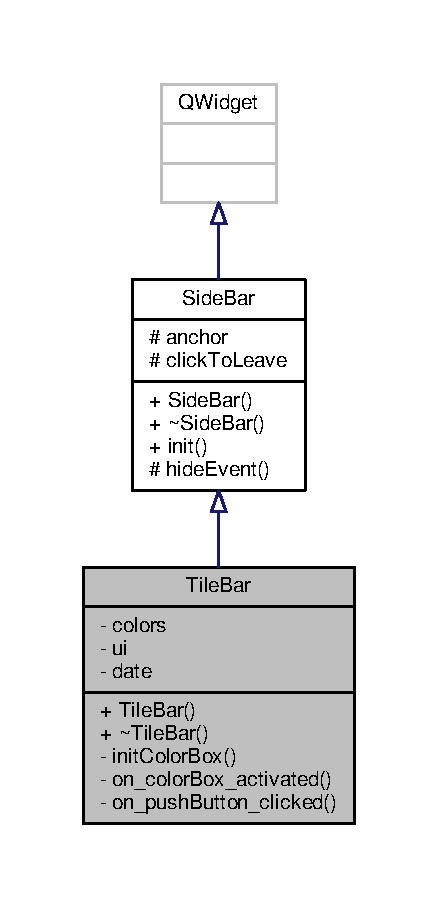
\includegraphics[width=210pt]{classTileBar__inherit__graph}
\end{center}
\end{figure}


Collaboration diagram for Tile\+Bar\+:
\nopagebreak
\begin{figure}[H]
\begin{center}
\leavevmode
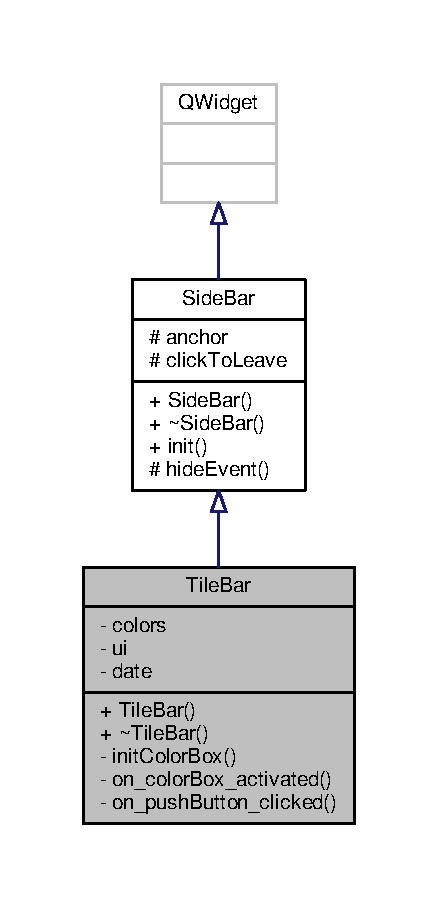
\includegraphics[width=210pt]{classTileBar__coll__graph}
\end{center}
\end{figure}
\subsection*{Public Member Functions}
\begin{DoxyCompactItemize}
\item 
\hyperlink{classTileBar_a4bbcd770768cb9a6b9635a9fa9392c9d}{Tile\+Bar} (Q\+Widget $\ast$\hyperlink{classSideBar_a0a6a0df257a08bdf785aeb155870efbc}{anchor}, Q\+Date \+\_\+date, Q\+Widget $\ast$parent=0)
\item 
\hyperlink{classTileBar_a435ad278c596c263b3b4e8e8b7bcea9d}{$\sim$\+Tile\+Bar} ()
\end{DoxyCompactItemize}
\subsection*{Private Slots}
\begin{DoxyCompactItemize}
\item 
void \hyperlink{classTileBar_a5c8d5cbdb4610d3d789317e55b048518}{on\+\_\+color\+Box\+\_\+activated} (int index)
\item 
void \hyperlink{classTileBar_af52d88e5b064071a70cda73e2539e64d}{on\+\_\+push\+Button\+\_\+clicked} (bool checked)
\end{DoxyCompactItemize}
\subsection*{Private Member Functions}
\begin{DoxyCompactItemize}
\item 
void \hyperlink{classTileBar_a13f8fb66568b7db9a6fc98c5aba1f6be}{init\+Color\+Box} ()
\end{DoxyCompactItemize}
\subsection*{Private Attributes}
\begin{DoxyCompactItemize}
\item 
const Q\+Color \hyperlink{classTileBar_ad6b37a17e07144010de05ac085610b9c}{colors} \mbox{[}4\mbox{]}
\item 
Ui\+::\+Tile\+Bar $\ast$ \hyperlink{classTileBar_a7f7a973a27b533d59e50a616d43e6ca8}{ui}
\item 
Q\+Date \hyperlink{classTileBar_ad7b85692977e160a39147db32cf7f735}{date}
\end{DoxyCompactItemize}
\subsection*{Additional Inherited Members}


\subsection{Detailed Description}
The side bar besides a day in the calendar. 

\subsection{Constructor \& Destructor Documentation}
\index{Tile\+Bar@{Tile\+Bar}!Tile\+Bar@{Tile\+Bar}}
\index{Tile\+Bar@{Tile\+Bar}!Tile\+Bar@{Tile\+Bar}}
\subsubsection[{\texorpdfstring{Tile\+Bar(\+Q\+Widget $\ast$anchor, Q\+Date \+\_\+date, Q\+Widget $\ast$parent=0)}{TileBar(QWidget *anchor, QDate _date, QWidget *parent=0)}}]{\setlength{\rightskip}{0pt plus 5cm}Tile\+Bar\+::\+Tile\+Bar (
\begin{DoxyParamCaption}
\item[{Q\+Widget $\ast$}]{anchor, }
\item[{Q\+Date}]{\+\_\+date, }
\item[{Q\+Widget $\ast$}]{parent = {\ttfamily 0}}
\end{DoxyParamCaption}
)\hspace{0.3cm}{\ttfamily [explicit]}}\hypertarget{classTileBar_a4bbcd770768cb9a6b9635a9fa9392c9d}{}\label{classTileBar_a4bbcd770768cb9a6b9635a9fa9392c9d}
\index{Tile\+Bar@{Tile\+Bar}!````~Tile\+Bar@{$\sim$\+Tile\+Bar}}
\index{````~Tile\+Bar@{$\sim$\+Tile\+Bar}!Tile\+Bar@{Tile\+Bar}}
\subsubsection[{\texorpdfstring{$\sim$\+Tile\+Bar()}{~TileBar()}}]{\setlength{\rightskip}{0pt plus 5cm}Tile\+Bar\+::$\sim$\+Tile\+Bar (
\begin{DoxyParamCaption}
{}
\end{DoxyParamCaption}
)}\hypertarget{classTileBar_a435ad278c596c263b3b4e8e8b7bcea9d}{}\label{classTileBar_a435ad278c596c263b3b4e8e8b7bcea9d}


\subsection{Member Function Documentation}
\index{Tile\+Bar@{Tile\+Bar}!init\+Color\+Box@{init\+Color\+Box}}
\index{init\+Color\+Box@{init\+Color\+Box}!Tile\+Bar@{Tile\+Bar}}
\subsubsection[{\texorpdfstring{init\+Color\+Box()}{initColorBox()}}]{\setlength{\rightskip}{0pt plus 5cm}void Tile\+Bar\+::init\+Color\+Box (
\begin{DoxyParamCaption}
{}
\end{DoxyParamCaption}
)\hspace{0.3cm}{\ttfamily [private]}}\hypertarget{classTileBar_a13f8fb66568b7db9a6fc98c5aba1f6be}{}\label{classTileBar_a13f8fb66568b7db9a6fc98c5aba1f6be}
\index{Tile\+Bar@{Tile\+Bar}!on\+\_\+color\+Box\+\_\+activated@{on\+\_\+color\+Box\+\_\+activated}}
\index{on\+\_\+color\+Box\+\_\+activated@{on\+\_\+color\+Box\+\_\+activated}!Tile\+Bar@{Tile\+Bar}}
\subsubsection[{\texorpdfstring{on\+\_\+color\+Box\+\_\+activated}{on_colorBox_activated}}]{\setlength{\rightskip}{0pt plus 5cm}void Tile\+Bar\+::on\+\_\+color\+Box\+\_\+activated (
\begin{DoxyParamCaption}
\item[{int}]{index}
\end{DoxyParamCaption}
)\hspace{0.3cm}{\ttfamily [private]}, {\ttfamily [slot]}}\hypertarget{classTileBar_a5c8d5cbdb4610d3d789317e55b048518}{}\label{classTileBar_a5c8d5cbdb4610d3d789317e55b048518}
\index{Tile\+Bar@{Tile\+Bar}!on\+\_\+push\+Button\+\_\+clicked@{on\+\_\+push\+Button\+\_\+clicked}}
\index{on\+\_\+push\+Button\+\_\+clicked@{on\+\_\+push\+Button\+\_\+clicked}!Tile\+Bar@{Tile\+Bar}}
\subsubsection[{\texorpdfstring{on\+\_\+push\+Button\+\_\+clicked}{on_pushButton_clicked}}]{\setlength{\rightskip}{0pt plus 5cm}void Tile\+Bar\+::on\+\_\+push\+Button\+\_\+clicked (
\begin{DoxyParamCaption}
\item[{bool}]{checked}
\end{DoxyParamCaption}
)\hspace{0.3cm}{\ttfamily [private]}, {\ttfamily [slot]}}\hypertarget{classTileBar_af52d88e5b064071a70cda73e2539e64d}{}\label{classTileBar_af52d88e5b064071a70cda73e2539e64d}


\subsection{Member Data Documentation}
\index{Tile\+Bar@{Tile\+Bar}!colors@{colors}}
\index{colors@{colors}!Tile\+Bar@{Tile\+Bar}}
\subsubsection[{\texorpdfstring{colors}{colors}}]{\setlength{\rightskip}{0pt plus 5cm}const Q\+Color Tile\+Bar\+::colors\mbox{[}4\mbox{]}\hspace{0.3cm}{\ttfamily [private]}}\hypertarget{classTileBar_ad6b37a17e07144010de05ac085610b9c}{}\label{classTileBar_ad6b37a17e07144010de05ac085610b9c}
{\bfseries Initial value\+:}
\begin{DoxyCode}
= \{
        QColor(0xE0, 0xFF, 0x85, 0xD0),
        QColor(0xFF, 0x00, 0x00, 0xD0),
        QColor(0x00, 0xFF, 0x00, 0xD0),
        QColor(0x00, 0x00, 0xFF, 0xD0)
    \}
\end{DoxyCode}
\index{Tile\+Bar@{Tile\+Bar}!date@{date}}
\index{date@{date}!Tile\+Bar@{Tile\+Bar}}
\subsubsection[{\texorpdfstring{date}{date}}]{\setlength{\rightskip}{0pt plus 5cm}Q\+Date Tile\+Bar\+::date\hspace{0.3cm}{\ttfamily [private]}}\hypertarget{classTileBar_ad7b85692977e160a39147db32cf7f735}{}\label{classTileBar_ad7b85692977e160a39147db32cf7f735}
\index{Tile\+Bar@{Tile\+Bar}!ui@{ui}}
\index{ui@{ui}!Tile\+Bar@{Tile\+Bar}}
\subsubsection[{\texorpdfstring{ui}{ui}}]{\setlength{\rightskip}{0pt plus 5cm}Ui\+::\+Tile\+Bar$\ast$ Tile\+Bar\+::ui\hspace{0.3cm}{\ttfamily [private]}}\hypertarget{classTileBar_a7f7a973a27b533d59e50a616d43e6ca8}{}\label{classTileBar_a7f7a973a27b533d59e50a616d43e6ca8}


The documentation for this class was generated from the following files\+:\begin{DoxyCompactItemize}
\item 
\hyperlink{tilebar_8h}{tilebar.\+h}\item 
\hyperlink{tilebar_8cpp}{tilebar.\+cpp}\end{DoxyCompactItemize}

\chapter{File Documentation}
\hypertarget{data_8cpp}{}\section{data.\+cpp File Reference}
\label{data_8cpp}\index{data.\+cpp@{data.\+cpp}}
{\ttfamily \#include $<$Q\+File$>$}\\*
{\ttfamily \#include $<$Q\+Pair$>$}\\*
{\ttfamily \#include $<$Q\+Debug$>$}\\*
{\ttfamily \#include $<$Q\+I\+O\+Device$>$}\\*
{\ttfamily \#include $<$Q\+Json\+Document$>$}\\*
{\ttfamily \#include \char`\"{}data.\+h\char`\"{}}\\*
{\ttfamily \#include \char`\"{}task.\+h\char`\"{}}\\*
{\ttfamily \#include \char`\"{}file.\+h\char`\"{}}\\*
Include dependency graph for data.\+cpp\+:
\nopagebreak
\begin{figure}[H]
\begin{center}
\leavevmode
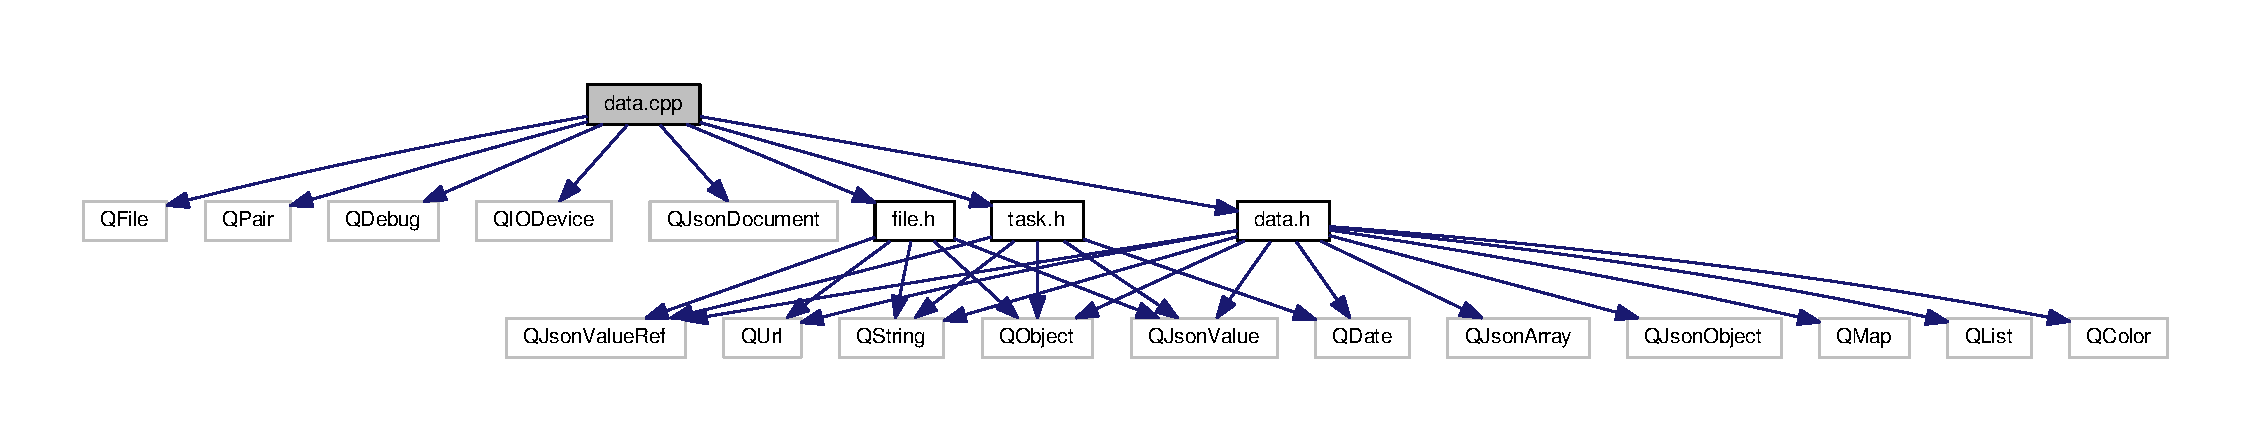
\includegraphics[width=350pt]{data_8cpp__incl}
\end{center}
\end{figure}

\hypertarget{data_8h}{}\section{data.\+h File Reference}
\label{data_8h}\index{data.\+h@{data.\+h}}
{\ttfamily \#include $<$Q\+Url$>$}\\*
{\ttfamily \#include $<$Q\+Map$>$}\\*
{\ttfamily \#include $<$Q\+List$>$}\\*
{\ttfamily \#include $<$Q\+Date$>$}\\*
{\ttfamily \#include $<$Q\+Color$>$}\\*
{\ttfamily \#include $<$Q\+String$>$}\\*
{\ttfamily \#include $<$Q\+Object$>$}\\*
{\ttfamily \#include $<$Q\+Json\+Value$>$}\\*
{\ttfamily \#include $<$Q\+Json\+Array$>$}\\*
{\ttfamily \#include $<$Q\+Json\+Object$>$}\\*
{\ttfamily \#include $<$Q\+Json\+Value\+Ref$>$}\\*
Include dependency graph for data.\+h\+:
\nopagebreak
\begin{figure}[H]
\begin{center}
\leavevmode
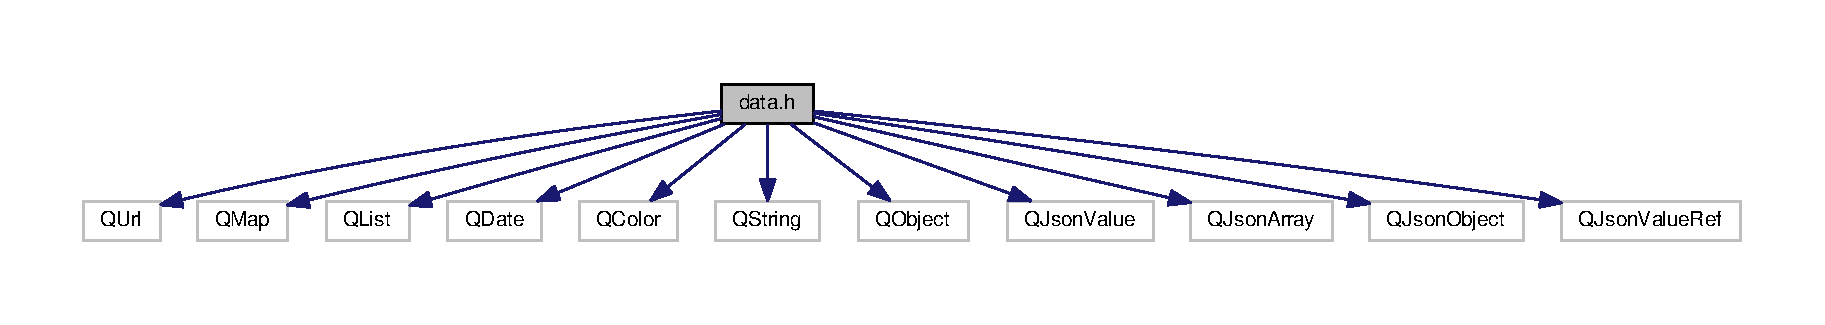
\includegraphics[width=350pt]{data_8h__incl}
\end{center}
\end{figure}
This graph shows which files directly or indirectly include this file\+:
\nopagebreak
\begin{figure}[H]
\begin{center}
\leavevmode
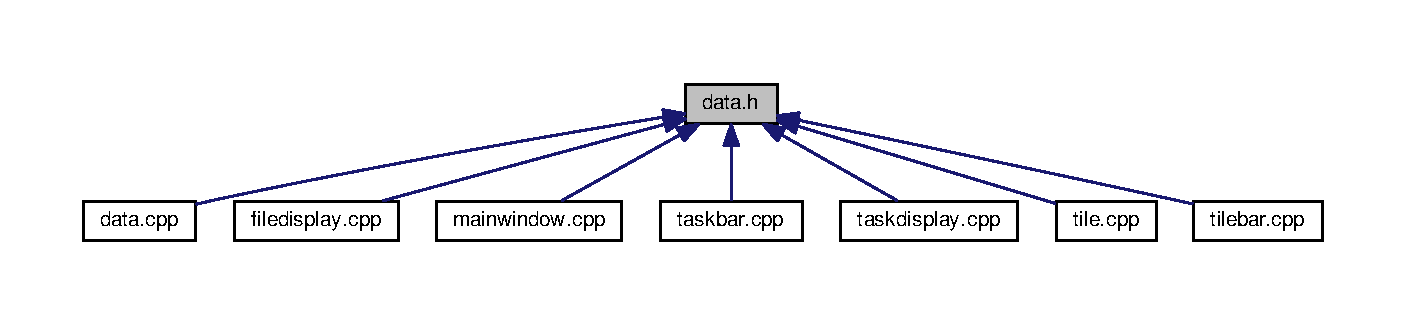
\includegraphics[width=350pt]{data_8h__dep__incl}
\end{center}
\end{figure}
\subsection*{Classes}
\begin{DoxyCompactItemize}
\item 
class \hyperlink{classData}{Data}
\begin{DoxyCompactList}\small\item\em Manage all user data and save it as J\+S\+ON format. \end{DoxyCompactList}\end{DoxyCompactItemize}

\hypertarget{dragdata_8cpp}{}\section{dragdata.\+cpp File Reference}
\label{dragdata_8cpp}\index{dragdata.\+cpp@{dragdata.\+cpp}}
{\ttfamily \#include $<$Q\+Dir$>$}\\*
{\ttfamily \#include $<$Q\+Url$>$}\\*
{\ttfamily \#include $<$Q\+File$>$}\\*
{\ttfamily \#include $<$Q\+Debug$>$}\\*
{\ttfamily \#include $<$Q\+I\+O\+Device$>$}\\*
{\ttfamily \#include $<$Q\+File\+Info$>$}\\*
{\ttfamily \#include $<$Q\+Byte\+Array$>$}\\*
{\ttfamily \#include \char`\"{}dragdata.\+h\char`\"{}}\\*
Include dependency graph for dragdata.\+cpp\+:
\nopagebreak
\begin{figure}[H]
\begin{center}
\leavevmode
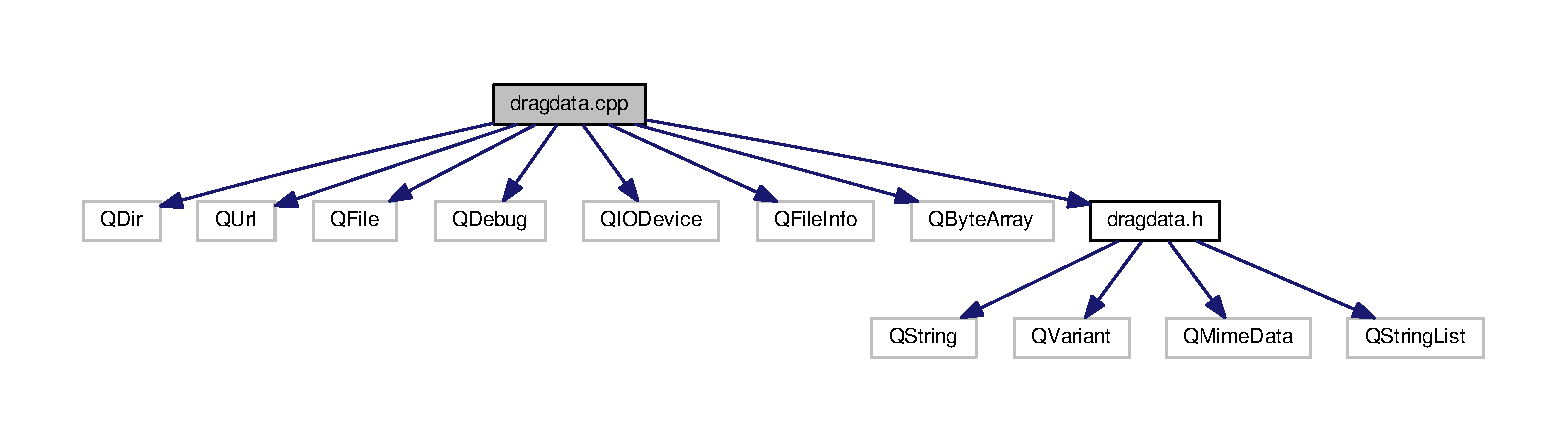
\includegraphics[width=350pt]{dragdata_8cpp__incl}
\end{center}
\end{figure}

\hypertarget{dragdata_8h}{}\section{dragdata.\+h File Reference}
\label{dragdata_8h}\index{dragdata.\+h@{dragdata.\+h}}
{\ttfamily \#include $<$Q\+String$>$}\\*
{\ttfamily \#include $<$Q\+Variant$>$}\\*
{\ttfamily \#include $<$Q\+Mime\+Data$>$}\\*
{\ttfamily \#include $<$Q\+String\+List$>$}\\*
Include dependency graph for dragdata.\+h\+:
\nopagebreak
\begin{figure}[H]
\begin{center}
\leavevmode
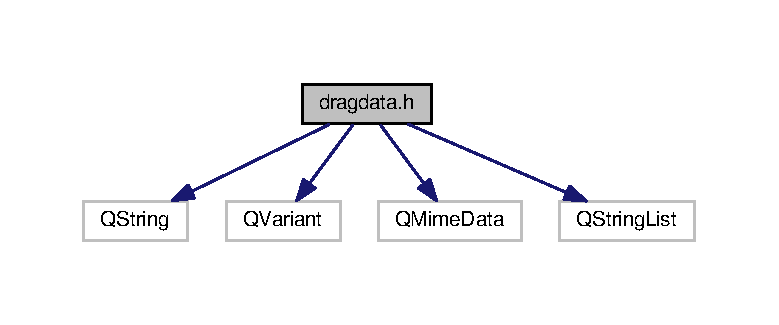
\includegraphics[width=350pt]{dragdata_8h__incl}
\end{center}
\end{figure}
This graph shows which files directly or indirectly include this file\+:
\nopagebreak
\begin{figure}[H]
\begin{center}
\leavevmode
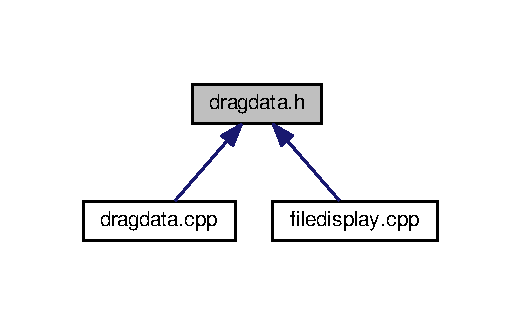
\includegraphics[width=250pt]{dragdata_8h__dep__incl}
\end{center}
\end{figure}
\subsection*{Classes}
\begin{DoxyCompactItemize}
\item 
class \hyperlink{classDragData}{Drag\+Data}
\begin{DoxyCompactList}\small\item\em Create a file and return its url when requested. \end{DoxyCompactList}\end{DoxyCompactItemize}

\hypertarget{file_8cpp}{}\section{file.\+cpp File Reference}
\label{file_8cpp}\index{file.\+cpp@{file.\+cpp}}
{\ttfamily \#include $<$Q\+File$>$}\\*
{\ttfamily \#include $<$Q\+I\+O\+Device$>$}\\*
{\ttfamily \#include $<$Q\+Json\+Object$>$}\\*
{\ttfamily \#include \char`\"{}file.\+h\char`\"{}}\\*
Include dependency graph for file.\+cpp\+:
\nopagebreak
\begin{figure}[H]
\begin{center}
\leavevmode
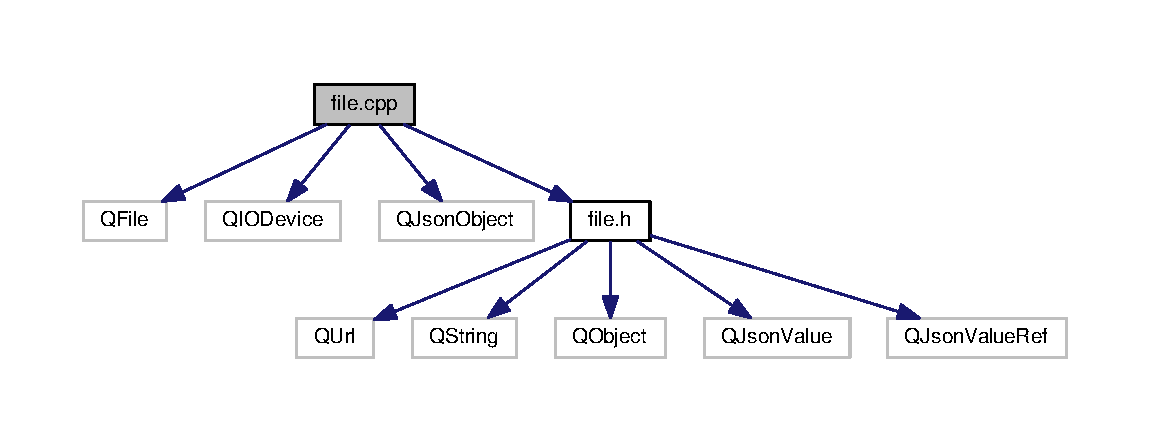
\includegraphics[width=350pt]{file_8cpp__incl}
\end{center}
\end{figure}

\hypertarget{file_8h}{}\section{file.\+h File Reference}
\label{file_8h}\index{file.\+h@{file.\+h}}
{\ttfamily \#include $<$Q\+Url$>$}\\*
{\ttfamily \#include $<$Q\+String$>$}\\*
{\ttfamily \#include $<$Q\+Object$>$}\\*
{\ttfamily \#include $<$Q\+Json\+Value$>$}\\*
{\ttfamily \#include $<$Q\+Json\+Value\+Ref$>$}\\*
Include dependency graph for file.\+h\+:
\nopagebreak
\begin{figure}[H]
\begin{center}
\leavevmode
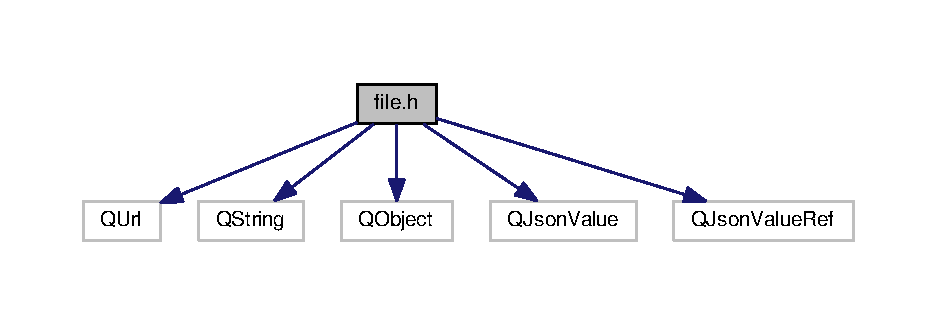
\includegraphics[width=350pt]{file_8h__incl}
\end{center}
\end{figure}
This graph shows which files directly or indirectly include this file\+:
\nopagebreak
\begin{figure}[H]
\begin{center}
\leavevmode
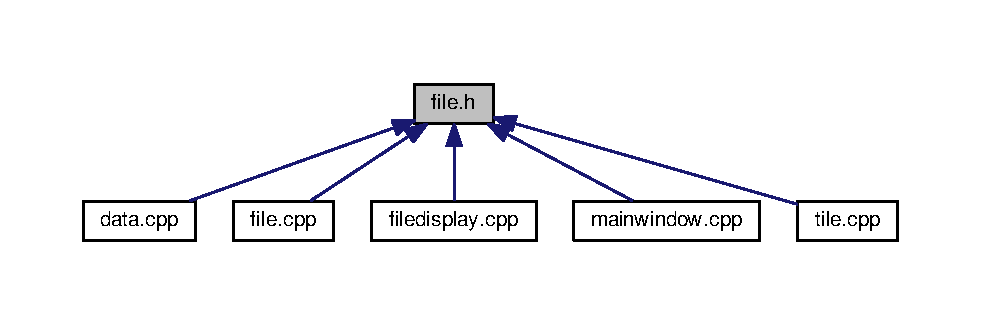
\includegraphics[width=350pt]{file_8h__dep__incl}
\end{center}
\end{figure}
\subsection*{Classes}
\begin{DoxyCompactItemize}
\item 
class \hyperlink{classFile}{File}
\begin{DoxyCompactList}\small\item\em A file dragged in by user. Encode its content in Base64. \end{DoxyCompactList}\end{DoxyCompactItemize}

\hypertarget{filedisplay_8cpp}{}\section{filedisplay.\+cpp File Reference}
\label{filedisplay_8cpp}\index{filedisplay.\+cpp@{filedisplay.\+cpp}}
{\ttfamily \#include $<$Q\+Drag$>$}\\*
{\ttfamily \#include $<$Q\+Debug$>$}\\*
{\ttfamily \#include $<$Q\+Label$>$}\\*
{\ttfamily \#include $<$Q\+String$>$}\\*
{\ttfamily \#include $<$Q\+Pixmap$>$}\\*
{\ttfamily \#include \char`\"{}data.\+h\char`\"{}}\\*
{\ttfamily \#include \char`\"{}file.\+h\char`\"{}}\\*
{\ttfamily \#include \char`\"{}html.\+h\char`\"{}}\\*
{\ttfamily \#include \char`\"{}dragdata.\+h\char`\"{}}\\*
{\ttfamily \#include \char`\"{}mainwindow.\+h\char`\"{}}\\*
{\ttfamily \#include \char`\"{}filedisplay.\+h\char`\"{}}\\*
{\ttfamily \#include \char`\"{}labelwithclick.\+h\char`\"{}}\\*
{\ttfamily \#include \char`\"{}ui\+\_\+filedisplay.\+h\char`\"{}}\\*
Include dependency graph for filedisplay.\+cpp\+:
\nopagebreak
\begin{figure}[H]
\begin{center}
\leavevmode
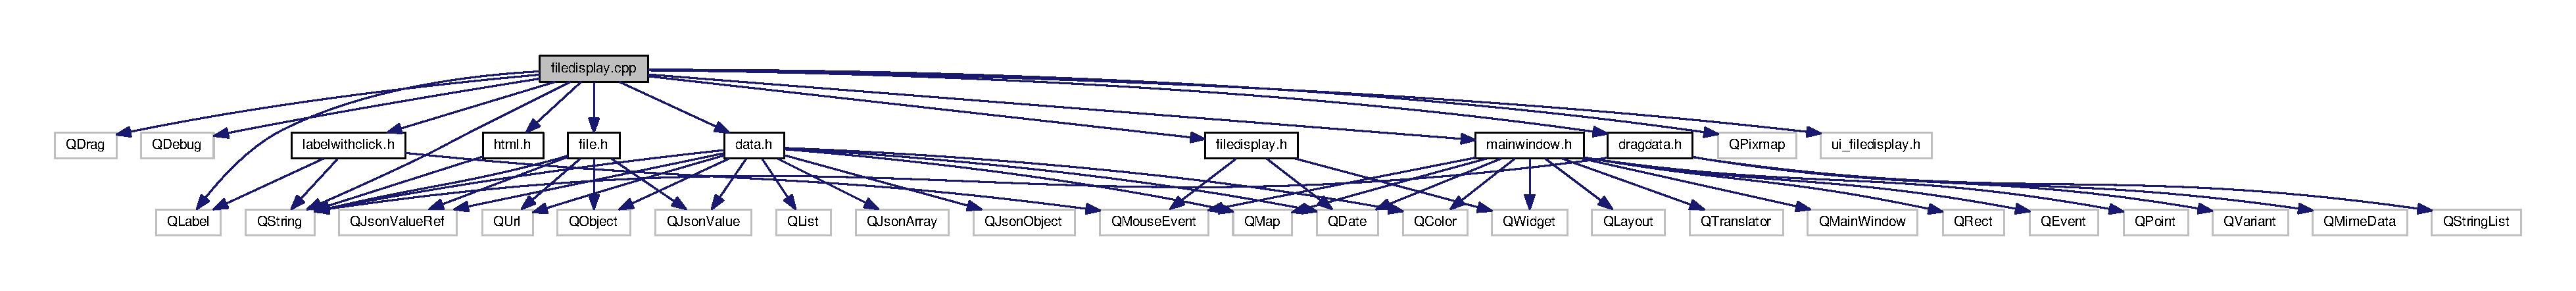
\includegraphics[width=350pt]{filedisplay_8cpp__incl}
\end{center}
\end{figure}

\hypertarget{filedisplay_8h}{}\section{filedisplay.\+h File Reference}
\label{filedisplay_8h}\index{filedisplay.\+h@{filedisplay.\+h}}
{\ttfamily \#include $<$Q\+Date$>$}\\*
{\ttfamily \#include $<$Q\+Widget$>$}\\*
{\ttfamily \#include $<$Q\+Mouse\+Event$>$}\\*
Include dependency graph for filedisplay.\+h\+:
\nopagebreak
\begin{figure}[H]
\begin{center}
\leavevmode
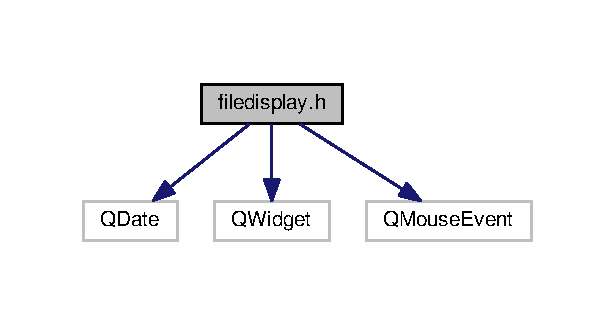
\includegraphics[width=295pt]{filedisplay_8h__incl}
\end{center}
\end{figure}
This graph shows which files directly or indirectly include this file\+:
\nopagebreak
\begin{figure}[H]
\begin{center}
\leavevmode
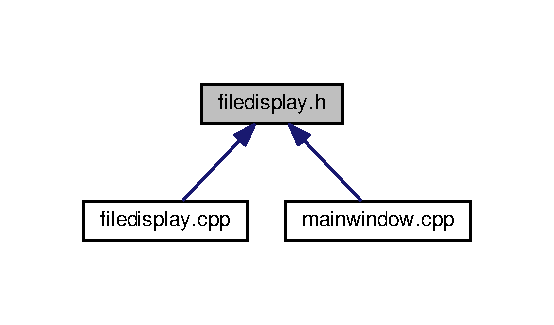
\includegraphics[width=266pt]{filedisplay_8h__dep__incl}
\end{center}
\end{figure}
\subsection*{Classes}
\begin{DoxyCompactItemize}
\item 
class \hyperlink{classFileDisplay}{File\+Display}
\begin{DoxyCompactList}\small\item\em Display a file dragged in by user. \end{DoxyCompactList}\end{DoxyCompactItemize}
\subsection*{Namespaces}
\begin{DoxyCompactItemize}
\item 
 \hyperlink{namespaceUi}{Ui}
\end{DoxyCompactItemize}

\hypertarget{help_8cpp}{}\section{help.\+cpp File Reference}
\label{help_8cpp}\index{help.\+cpp@{help.\+cpp}}
{\ttfamily \#include $<$Q\+Debug$>$}\\*
{\ttfamily \#include $<$Q\+Dialog\+Button\+Box$>$}\\*
{\ttfamily \#include \char`\"{}help.\+h\char`\"{}}\\*
{\ttfamily \#include \char`\"{}ui\+\_\+help.\+h\char`\"{}}\\*
Include dependency graph for help.\+cpp\+:
\nopagebreak
\begin{figure}[H]
\begin{center}
\leavevmode
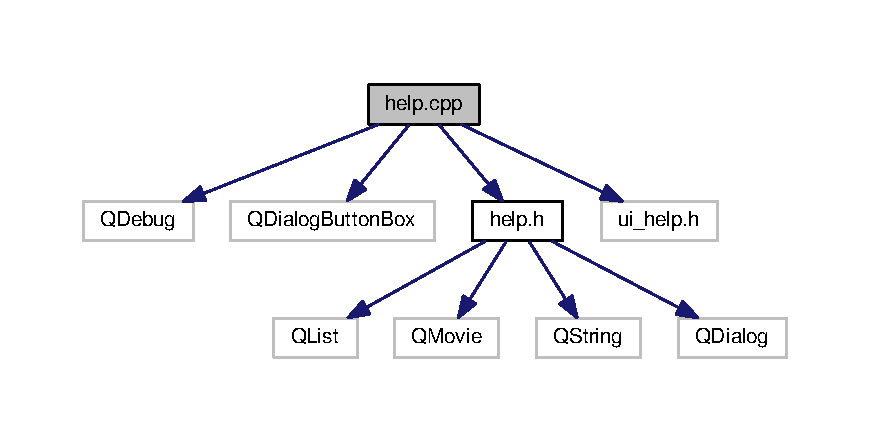
\includegraphics[width=350pt]{help_8cpp__incl}
\end{center}
\end{figure}

\hypertarget{help_8h}{}\section{help.\+h File Reference}
\label{help_8h}\index{help.\+h@{help.\+h}}
{\ttfamily \#include $<$Q\+List$>$}\\*
{\ttfamily \#include $<$Q\+Movie$>$}\\*
{\ttfamily \#include $<$Q\+String$>$}\\*
{\ttfamily \#include $<$Q\+Dialog$>$}\\*
Include dependency graph for help.\+h\+:
\nopagebreak
\begin{figure}[H]
\begin{center}
\leavevmode
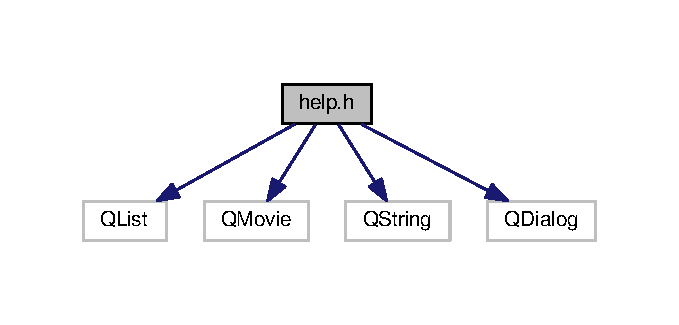
\includegraphics[width=326pt]{help_8h__incl}
\end{center}
\end{figure}
This graph shows which files directly or indirectly include this file\+:
\nopagebreak
\begin{figure}[H]
\begin{center}
\leavevmode
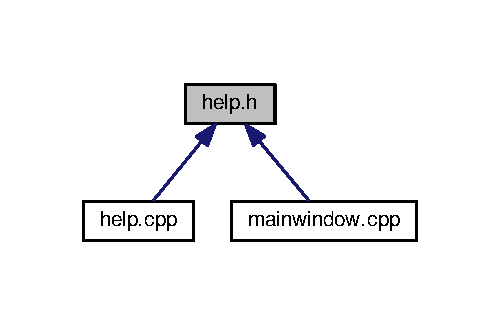
\includegraphics[width=240pt]{help_8h__dep__incl}
\end{center}
\end{figure}
\subsection*{Classes}
\begin{DoxyCompactItemize}
\item 
class \hyperlink{classHelp}{Help}
\end{DoxyCompactItemize}
\subsection*{Namespaces}
\begin{DoxyCompactItemize}
\item 
 \hyperlink{namespaceUi}{Ui}
\end{DoxyCompactItemize}

\hypertarget{html_8cpp}{}\section{html.\+cpp File Reference}
\label{html_8cpp}\index{html.\+cpp@{html.\+cpp}}
{\ttfamily \#include \char`\"{}html.\+h\char`\"{}}\\*
Include dependency graph for html.\+cpp\+:
\nopagebreak
\begin{figure}[H]
\begin{center}
\leavevmode
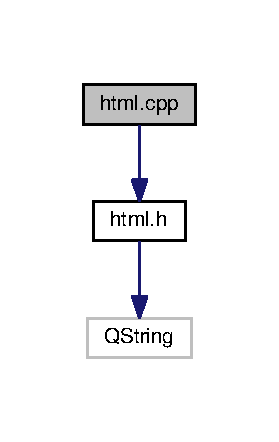
\includegraphics[width=134pt]{html_8cpp__incl}
\end{center}
\end{figure}

\hypertarget{html_8h}{}\section{html.\+h File Reference}
\label{html_8h}\index{html.\+h@{html.\+h}}
{\ttfamily \#include $<$Q\+String$>$}\\*
Include dependency graph for html.\+h\+:
\nopagebreak
\begin{figure}[H]
\begin{center}
\leavevmode
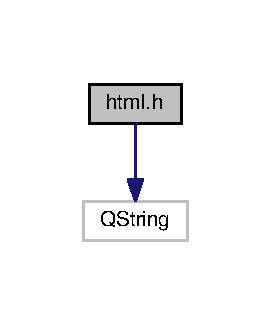
\includegraphics[width=130pt]{html_8h__incl}
\end{center}
\end{figure}
This graph shows which files directly or indirectly include this file\+:
\nopagebreak
\begin{figure}[H]
\begin{center}
\leavevmode
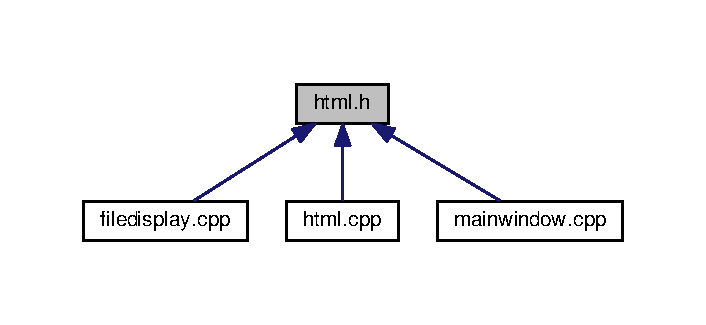
\includegraphics[width=339pt]{html_8h__dep__incl}
\end{center}
\end{figure}
\subsection*{Classes}
\begin{DoxyCompactItemize}
\item 
class \hyperlink{classHtml}{Html}
\begin{DoxyCompactList}\small\item\em Add H\+T\+ML flavor to a string. \end{DoxyCompactList}\end{DoxyCompactItemize}

\hypertarget{labelwithclick_8cpp}{}\section{labelwithclick.\+cpp File Reference}
\label{labelwithclick_8cpp}\index{labelwithclick.\+cpp@{labelwithclick.\+cpp}}
{\ttfamily \#include \char`\"{}mainwindow.\+h\char`\"{}}\\*
{\ttfamily \#include \char`\"{}labelwithclick.\+h\char`\"{}}\\*
Include dependency graph for labelwithclick.\+cpp\+:
\nopagebreak
\begin{figure}[H]
\begin{center}
\leavevmode
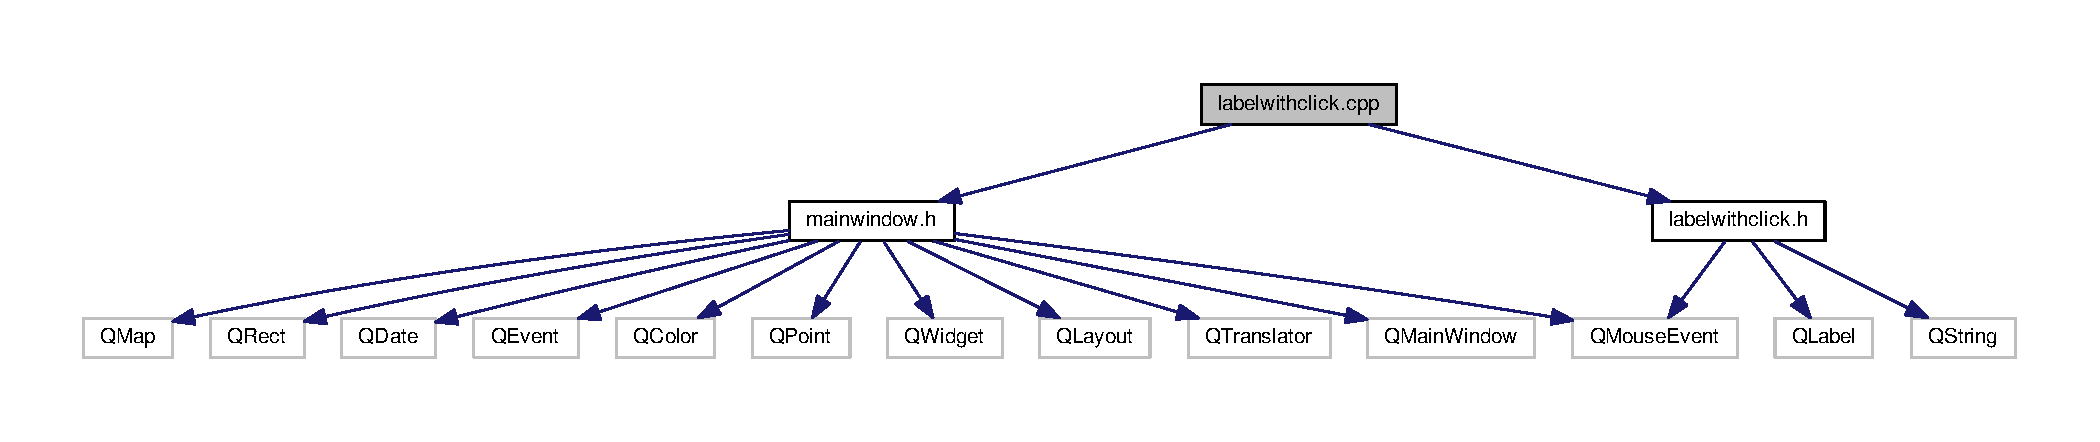
\includegraphics[width=350pt]{labelwithclick_8cpp__incl}
\end{center}
\end{figure}

\hypertarget{labelwithclick_8h}{}\section{labelwithclick.\+h File Reference}
\label{labelwithclick_8h}\index{labelwithclick.\+h@{labelwithclick.\+h}}
{\ttfamily \#include $<$Q\+Label$>$}\\*
{\ttfamily \#include $<$Q\+String$>$}\\*
{\ttfamily \#include $<$Q\+Mouse\+Event$>$}\\*
Include dependency graph for labelwithclick.\+h\+:
\nopagebreak
\begin{figure}[H]
\begin{center}
\leavevmode
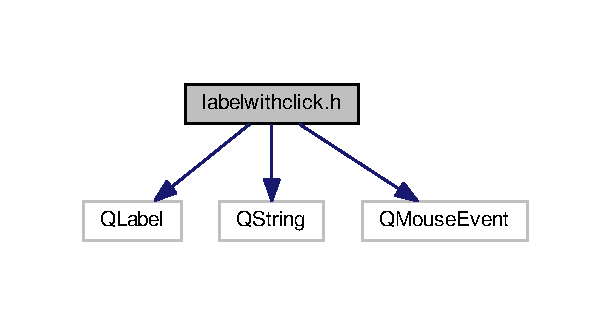
\includegraphics[width=293pt]{labelwithclick_8h__incl}
\end{center}
\end{figure}
This graph shows which files directly or indirectly include this file\+:
\nopagebreak
\begin{figure}[H]
\begin{center}
\leavevmode
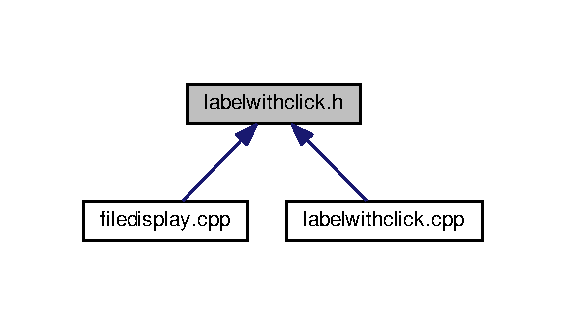
\includegraphics[width=272pt]{labelwithclick_8h__dep__incl}
\end{center}
\end{figure}
\subsection*{Classes}
\begin{DoxyCompactItemize}
\item 
class \hyperlink{classLabelWithClick}{Label\+With\+Click}
\end{DoxyCompactItemize}

\hypertarget{main_8cpp}{}\section{main.\+cpp File Reference}
\label{main_8cpp}\index{main.\+cpp@{main.\+cpp}}
{\ttfamily \#include $<$Q\+Application$>$}\\*
{\ttfamily \#include \char`\"{}mainwindow.\+h\char`\"{}}\\*
Include dependency graph for main.\+cpp\+:
\nopagebreak
\begin{figure}[H]
\begin{center}
\leavevmode
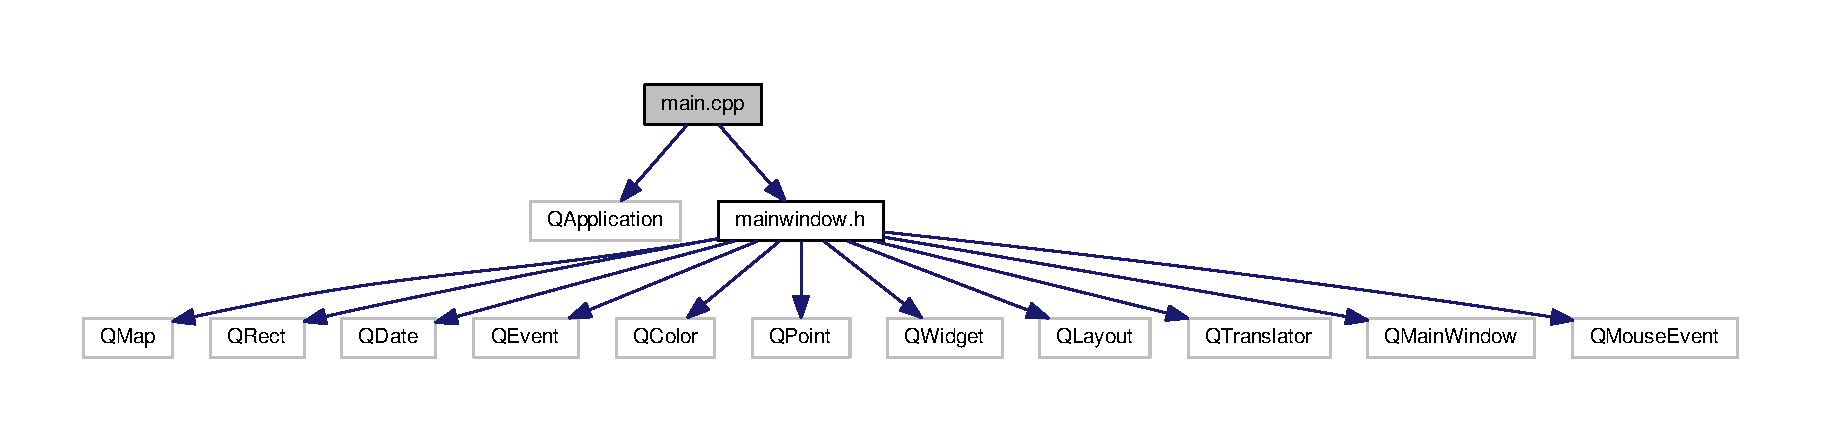
\includegraphics[width=350pt]{main_8cpp__incl}
\end{center}
\end{figure}
\subsection*{Functions}
\begin{DoxyCompactItemize}
\item 
int \hyperlink{main_8cpp_a0ddf1224851353fc92bfbff6f499fa97}{main} (int argc, char $\ast$argv\mbox{[}$\,$\mbox{]})
\end{DoxyCompactItemize}


\subsection{Function Documentation}
\index{main.\+cpp@{main.\+cpp}!main@{main}}
\index{main@{main}!main.\+cpp@{main.\+cpp}}
\subsubsection[{\texorpdfstring{main(int argc, char $\ast$argv[])}{main(int argc, char *argv[])}}]{\setlength{\rightskip}{0pt plus 5cm}int main (
\begin{DoxyParamCaption}
\item[{int}]{argc, }
\item[{char $\ast$}]{argv\mbox{[}$\,$\mbox{]}}
\end{DoxyParamCaption}
)}\hypertarget{main_8cpp_a0ddf1224851353fc92bfbff6f499fa97}{}\label{main_8cpp_a0ddf1224851353fc92bfbff6f499fa97}

\hypertarget{mainwindow_8cpp}{}\section{mainwindow.\+cpp File Reference}
\label{mainwindow_8cpp}\index{mainwindow.\+cpp@{mainwindow.\+cpp}}
{\ttfamily \#include $<$algorithm$>$}\\*
{\ttfamily \#include $<$Q\+File$>$}\\*
{\ttfamily \#include $<$Q\+List$>$}\\*
{\ttfamily \#include $<$Q\+Icon$>$}\\*
{\ttfamily \#include $<$Q\+Rect$>$}\\*
{\ttfamily \#include $<$Q\+Brush$>$}\\*
{\ttfamily \#include $<$Q\+Label$>$}\\*
{\ttfamily \#include $<$Q\+Debug$>$}\\*
{\ttfamily \#include $<$Q\+Point$>$}\\*
{\ttfamily \#include $<$Q\+Region$>$}\\*
{\ttfamily \#include $<$Q\+Palette$>$}\\*
{\ttfamily \#include $<$Q\+Combo\+Box$>$}\\*
{\ttfamily \#include $<$Q\+Grid\+Layout$>$}\\*
{\ttfamily \#include $<$Q\+File\+Dialog$>$}\\*
{\ttfamily \#include $<$Q\+V\+Box\+Layout$>$}\\*
{\ttfamily \#include $<$Q\+Layout\+Item$>$}\\*
{\ttfamily \#include $<$Q\+Signal\+Mapper$>$}\\*
{\ttfamily \#include $<$Q\+Text\+Char\+Format$>$}\\*
{\ttfamily \#include $<$Q\+Calendar\+Widget$>$}\\*
{\ttfamily \#include \char`\"{}help.\+h\char`\"{}}\\*
{\ttfamily \#include \char`\"{}data.\+h\char`\"{}}\\*
{\ttfamily \#include \char`\"{}file.\+h\char`\"{}}\\*
{\ttfamily \#include \char`\"{}tile.\+h\char`\"{}}\\*
{\ttfamily \#include \char`\"{}html.\+h\char`\"{}}\\*
{\ttfamily \#include \char`\"{}ui\+\_\+tile.\+h\char`\"{}}\\*
{\ttfamily \#include \char`\"{}taskbar.\+h\char`\"{}}\\*
{\ttfamily \#include \char`\"{}tilebar.\+h\char`\"{}}\\*
{\ttfamily \#include \char`\"{}mainwindow.\+h\char`\"{}}\\*
{\ttfamily \#include \char`\"{}taskdisplay.\+h\char`\"{}}\\*
{\ttfamily \#include \char`\"{}filedisplay.\+h\char`\"{}}\\*
{\ttfamily \#include \char`\"{}ui\+\_\+mainwindow.\+h\char`\"{}}\\*
Include dependency graph for mainwindow.\+cpp\+:
\nopagebreak
\begin{figure}[H]
\begin{center}
\leavevmode
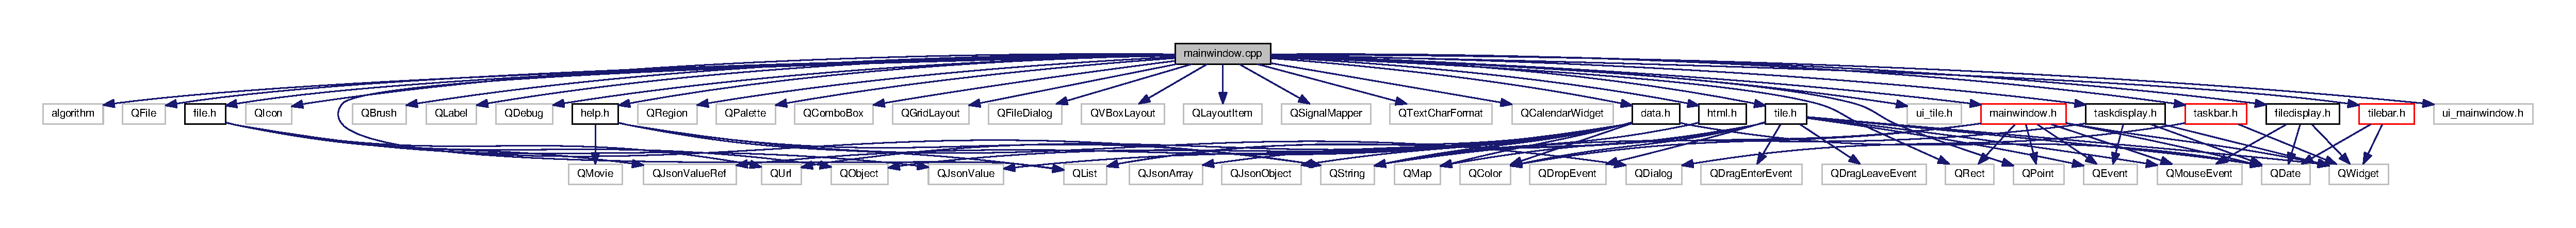
\includegraphics[width=350pt]{mainwindow_8cpp__incl}
\end{center}
\end{figure}

\hypertarget{mainwindow_8h}{}\section{mainwindow.\+h File Reference}
\label{mainwindow_8h}\index{mainwindow.\+h@{mainwindow.\+h}}
{\ttfamily \#include $<$Q\+Map$>$}\\*
{\ttfamily \#include $<$Q\+Rect$>$}\\*
{\ttfamily \#include $<$Q\+Date$>$}\\*
{\ttfamily \#include $<$Q\+Event$>$}\\*
{\ttfamily \#include $<$Q\+Color$>$}\\*
{\ttfamily \#include $<$Q\+Point$>$}\\*
{\ttfamily \#include $<$Q\+Widget$>$}\\*
{\ttfamily \#include $<$Q\+Layout$>$}\\*
{\ttfamily \#include $<$Q\+Translator$>$}\\*
{\ttfamily \#include $<$Q\+Main\+Window$>$}\\*
{\ttfamily \#include $<$Q\+Mouse\+Event$>$}\\*
Include dependency graph for mainwindow.\+h\+:
\nopagebreak
\begin{figure}[H]
\begin{center}
\leavevmode
\includegraphics[width=350pt]{mainwindow_8h__incl}
\end{center}
\end{figure}
This graph shows which files directly or indirectly include this file\+:
\nopagebreak
\begin{figure}[H]
\begin{center}
\leavevmode
\includegraphics[width=350pt]{mainwindow_8h__dep__incl}
\end{center}
\end{figure}
\subsection*{Classes}
\begin{DoxyCompactItemize}
\item 
class \hyperlink{classMainWindow}{Main\+Window}
\end{DoxyCompactItemize}
\subsection*{Namespaces}
\begin{DoxyCompactItemize}
\item 
 \hyperlink{namespaceUi}{Ui}
\end{DoxyCompactItemize}

\hypertarget{sidebar_8cpp}{}\section{sidebar.\+cpp File Reference}
\label{sidebar_8cpp}\index{sidebar.\+cpp@{sidebar.\+cpp}}
{\ttfamily \#include $<$Q\+Debug$>$}\\*
{\ttfamily \#include $<$Q\+Graphics\+Blur\+Effect$>$}\\*
{\ttfamily \#include \char`\"{}sidebar.\+h\char`\"{}}\\*
{\ttfamily \#include \char`\"{}mainwindow.\+h\char`\"{}}\\*
Include dependency graph for sidebar.\+cpp\+:
\nopagebreak
\begin{figure}[H]
\begin{center}
\leavevmode
\includegraphics[width=350pt]{sidebar_8cpp__incl}
\end{center}
\end{figure}

\hypertarget{sidebar_8h}{}\section{sidebar.\+h File Reference}
\label{sidebar_8h}\index{sidebar.\+h@{sidebar.\+h}}
{\ttfamily \#include $<$Q\+Widget$>$}\\*
Include dependency graph for sidebar.\+h\+:
\nopagebreak
\begin{figure}[H]
\begin{center}
\leavevmode
\includegraphics[width=136pt]{sidebar_8h__incl}
\end{center}
\end{figure}
This graph shows which files directly or indirectly include this file\+:
\nopagebreak
\begin{figure}[H]
\begin{center}
\leavevmode
\includegraphics[width=350pt]{sidebar_8h__dep__incl}
\end{center}
\end{figure}
\subsection*{Classes}
\begin{DoxyCompactItemize}
\item 
class \hyperlink{classSideBar}{Side\+Bar}
\begin{DoxyCompactList}\small\item\em Base class for side bar besides a day or a task. \end{DoxyCompactList}\end{DoxyCompactItemize}

\hypertarget{task_8cpp}{}\section{task.\+cpp File Reference}
\label{task_8cpp}\index{task.\+cpp@{task.\+cpp}}
{\ttfamily \#include $<$Q\+Debug$>$}\\*
{\ttfamily \#include $<$Q\+Json\+Array$>$}\\*
{\ttfamily \#include $<$Q\+Json\+Value$>$}\\*
{\ttfamily \#include $<$Q\+Json\+Object$>$}\\*
{\ttfamily \#include $<$Q\+Json\+Document$>$}\\*
{\ttfamily \#include \char`\"{}task.\+h\char`\"{}}\\*
Include dependency graph for task.\+cpp\+:
\nopagebreak
\begin{figure}[H]
\begin{center}
\leavevmode
\includegraphics[width=350pt]{task_8cpp__incl}
\end{center}
\end{figure}

\hypertarget{task_8h}{}\section{task.\+h File Reference}
\label{task_8h}\index{task.\+h@{task.\+h}}
{\ttfamily \#include $<$Q\+Date$>$}\\*
{\ttfamily \#include $<$Q\+String$>$}\\*
{\ttfamily \#include $<$Q\+Object$>$}\\*
{\ttfamily \#include $<$Q\+Json\+Value$>$}\\*
{\ttfamily \#include $<$Q\+Json\+Value\+Ref$>$}\\*
Include dependency graph for task.\+h\+:
\nopagebreak
\begin{figure}[H]
\begin{center}
\leavevmode
\includegraphics[width=350pt]{task_8h__incl}
\end{center}
\end{figure}
This graph shows which files directly or indirectly include this file\+:
\nopagebreak
\begin{figure}[H]
\begin{center}
\leavevmode
\includegraphics[width=350pt]{task_8h__dep__incl}
\end{center}
\end{figure}
\subsection*{Classes}
\begin{DoxyCompactItemize}
\item 
class \hyperlink{classTask}{Task}
\begin{DoxyCompactList}\small\item\em A task defined by user. \end{DoxyCompactList}\end{DoxyCompactItemize}

\hypertarget{taskbar_8cpp}{}\section{taskbar.\+cpp File Reference}
\label{taskbar_8cpp}\index{taskbar.\+cpp@{taskbar.\+cpp}}
{\ttfamily \#include $<$Q\+Rect$>$}\\*
{\ttfamily \#include $<$Q\+Debug$>$}\\*
{\ttfamily \#include $<$algorithm$>$}\\*
{\ttfamily \#include $<$Q\+Size\+Policy$>$}\\*
{\ttfamily \#include \char`\"{}data.\+h\char`\"{}}\\*
{\ttfamily \#include \char`\"{}task.\+h\char`\"{}}\\*
{\ttfamily \#include \char`\"{}taskbar.\+h\char`\"{}}\\*
{\ttfamily \#include \char`\"{}ui\+\_\+taskbar.\+h\char`\"{}}\\*
{\ttfamily \#include \char`\"{}mainwindow.\+h\char`\"{}}\\*
{\ttfamily \#include \char`\"{}taskdisplay.\+h\char`\"{}}\\*
Include dependency graph for taskbar.\+cpp\+:
\nopagebreak
\begin{figure}[H]
\begin{center}
\leavevmode
\includegraphics[width=350pt]{taskbar_8cpp__incl}
\end{center}
\end{figure}

\hypertarget{taskbar_8h}{}\section{taskbar.\+h File Reference}
\label{taskbar_8h}\index{taskbar.\+h@{taskbar.\+h}}
{\ttfamily \#include $<$Q\+Widget$>$}\\*
{\ttfamily \#include $<$Q\+Dialog$>$}\\*
{\ttfamily \#include \char`\"{}task.\+h\char`\"{}}\\*
{\ttfamily \#include \char`\"{}sidebar.\+h\char`\"{}}\\*
Include dependency graph for taskbar.\+h\+:
\nopagebreak
\begin{figure}[H]
\begin{center}
\leavevmode
\includegraphics[width=350pt]{taskbar_8h__incl}
\end{center}
\end{figure}
This graph shows which files directly or indirectly include this file\+:
\nopagebreak
\begin{figure}[H]
\begin{center}
\leavevmode
\includegraphics[width=256pt]{taskbar_8h__dep__incl}
\end{center}
\end{figure}
\subsection*{Classes}
\begin{DoxyCompactItemize}
\item 
class \hyperlink{classTaskBar}{Task\+Bar}
\begin{DoxyCompactList}\small\item\em Provide an interface for users to interact with tasks. \end{DoxyCompactList}\end{DoxyCompactItemize}
\subsection*{Namespaces}
\begin{DoxyCompactItemize}
\item 
 \hyperlink{namespaceUi}{Ui}
\end{DoxyCompactItemize}

\hypertarget{taskdisplay_8cpp}{}\section{taskdisplay.\+cpp File Reference}
\label{taskdisplay_8cpp}\index{taskdisplay.\+cpp@{taskdisplay.\+cpp}}
{\ttfamily \#include $<$Q\+Debug$>$}\\*
{\ttfamily \#include $<$Q\+Graphics\+Colorize\+Effect$>$}\\*
{\ttfamily \#include \char`\"{}tile.\+h\char`\"{}}\\*
{\ttfamily \#include \char`\"{}data.\+h\char`\"{}}\\*
{\ttfamily \#include \char`\"{}task.\+h\char`\"{}}\\*
{\ttfamily \#include \char`\"{}mainwindow.\+h\char`\"{}}\\*
{\ttfamily \#include \char`\"{}taskdisplay.\+h\char`\"{}}\\*
{\ttfamily \#include \char`\"{}ui\+\_\+taskdisplay.\+h\char`\"{}}\\*
Include dependency graph for taskdisplay.\+cpp\+:
\nopagebreak
\begin{figure}[H]
\begin{center}
\leavevmode
\includegraphics[width=350pt]{taskdisplay_8cpp__incl}
\end{center}
\end{figure}

\hypertarget{taskdisplay_8h}{}\section{taskdisplay.\+h File Reference}
\label{taskdisplay_8h}\index{taskdisplay.\+h@{taskdisplay.\+h}}
{\ttfamily \#include $<$Q\+Date$>$}\\*
{\ttfamily \#include $<$Q\+Event$>$}\\*
{\ttfamily \#include $<$Q\+String$>$}\\*
{\ttfamily \#include $<$Q\+Widget$>$}\\*
Include dependency graph for taskdisplay.\+h\+:
\nopagebreak
\begin{figure}[H]
\begin{center}
\leavevmode
\includegraphics[width=335pt]{taskdisplay_8h__incl}
\end{center}
\end{figure}
This graph shows which files directly or indirectly include this file\+:
\nopagebreak
\begin{figure}[H]
\begin{center}
\leavevmode
\includegraphics[width=350pt]{taskdisplay_8h__dep__incl}
\end{center}
\end{figure}
\subsection*{Classes}
\begin{DoxyCompactItemize}
\item 
class \hyperlink{classTaskDisplay}{Task\+Display}
\begin{DoxyCompactList}\small\item\em Display and edit a task. \end{DoxyCompactList}\end{DoxyCompactItemize}
\subsection*{Namespaces}
\begin{DoxyCompactItemize}
\item 
 \hyperlink{namespaceUi}{Ui}
\end{DoxyCompactItemize}

\hypertarget{tile_8cpp}{}\section{tile.\+cpp File Reference}
\label{tile_8cpp}\index{tile.\+cpp@{tile.\+cpp}}
{\ttfamily \#include $<$Q\+Url$>$}\\*
{\ttfamily \#include $<$Q\+List$>$}\\*
{\ttfamily \#include $<$Q\+File$>$}\\*
{\ttfamily \#include $<$Q\+Debug$>$}\\*
{\ttfamily \#include $<$Q\+Palette$>$}\\*
{\ttfamily \#include $<$Q\+File\+Info$>$}\\*
{\ttfamily \#include $<$Q\+Mime\+Data$>$}\\*
{\ttfamily \#include $<$Q\+Graphics\+Colorize\+Effect$>$}\\*
{\ttfamily \#include \char`\"{}data.\+h\char`\"{}}\\*
{\ttfamily \#include \char`\"{}file.\+h\char`\"{}}\\*
{\ttfamily \#include \char`\"{}tile.\+h\char`\"{}}\\*
{\ttfamily \#include \char`\"{}ui\+\_\+tile.\+h\char`\"{}}\\*
{\ttfamily \#include \char`\"{}mainwindow.\+h\char`\"{}}\\*
Include dependency graph for tile.\+cpp\+:
\nopagebreak
\begin{figure}[H]
\begin{center}
\leavevmode
\includegraphics[width=350pt]{tile_8cpp__incl}
\end{center}
\end{figure}

\hypertarget{tile_8h}{}\section{tile.\+h File Reference}
\label{tile_8h}\index{tile.\+h@{tile.\+h}}
{\ttfamily \#include $<$Q\+List$>$}\\*
{\ttfamily \#include $<$Q\+Date$>$}\\*
{\ttfamily \#include $<$Q\+Color$>$}\\*
{\ttfamily \#include $<$Q\+Event$>$}\\*
{\ttfamily \#include $<$Q\+String$>$}\\*
{\ttfamily \#include $<$Q\+Widget$>$}\\*
{\ttfamily \#include $<$Q\+Drop\+Event$>$}\\*
{\ttfamily \#include $<$Q\+Mouse\+Event$>$}\\*
{\ttfamily \#include $<$Q\+Drag\+Enter\+Event$>$}\\*
{\ttfamily \#include $<$Q\+Drag\+Leave\+Event$>$}\\*
Include dependency graph for tile.\+h\+:
\nopagebreak
\begin{figure}[H]
\begin{center}
\leavevmode
\includegraphics[width=350pt]{tile_8h__incl}
\end{center}
\end{figure}
This graph shows which files directly or indirectly include this file\+:
\nopagebreak
\begin{figure}[H]
\begin{center}
\leavevmode
\includegraphics[width=339pt]{tile_8h__dep__incl}
\end{center}
\end{figure}
\subsection*{Classes}
\begin{DoxyCompactItemize}
\item 
class \hyperlink{classTile}{Tile}
\begin{DoxyCompactList}\small\item\em A grid cell response for a day. \end{DoxyCompactList}\end{DoxyCompactItemize}
\subsection*{Namespaces}
\begin{DoxyCompactItemize}
\item 
 \hyperlink{namespaceUi}{Ui}
\end{DoxyCompactItemize}

\hypertarget{tilebar_8cpp}{}\section{tilebar.\+cpp File Reference}
\label{tilebar_8cpp}\index{tilebar.\+cpp@{tilebar.\+cpp}}
{\ttfamily \#include $<$Q\+Debug$>$}\\*
{\ttfamily \#include $<$Q\+Color$>$}\\*
{\ttfamily \#include $<$Q\+String$>$}\\*
{\ttfamily \#include \char`\"{}data.\+h\char`\"{}}\\*
{\ttfamily \#include \char`\"{}tilebar.\+h\char`\"{}}\\*
{\ttfamily \#include \char`\"{}mainwindow.\+h\char`\"{}}\\*
{\ttfamily \#include \char`\"{}ui\+\_\+tilebar.\+h\char`\"{}}\\*
Include dependency graph for tilebar.\+cpp\+:
\nopagebreak
\begin{figure}[H]
\begin{center}
\leavevmode
\includegraphics[width=350pt]{tilebar_8cpp__incl}
\end{center}
\end{figure}

\hypertarget{tilebar_8h}{}\section{tilebar.\+h File Reference}
\label{tilebar_8h}\index{tilebar.\+h@{tilebar.\+h}}
{\ttfamily \#include $<$Q\+Date$>$}\\*
{\ttfamily \#include $<$Q\+Widget$>$}\\*
{\ttfamily \#include \char`\"{}sidebar.\+h\char`\"{}}\\*
Include dependency graph for tilebar.\+h\+:
\nopagebreak
\begin{figure}[H]
\begin{center}
\leavevmode
\includegraphics[width=238pt]{tilebar_8h__incl}
\end{center}
\end{figure}
This graph shows which files directly or indirectly include this file\+:
\nopagebreak
\begin{figure}[H]
\begin{center}
\leavevmode
\includegraphics[width=249pt]{tilebar_8h__dep__incl}
\end{center}
\end{figure}
\subsection*{Classes}
\begin{DoxyCompactItemize}
\item 
class \hyperlink{classTileBar}{Tile\+Bar}
\begin{DoxyCompactList}\small\item\em The side bar besides a day in the calendar. \end{DoxyCompactList}\end{DoxyCompactItemize}
\subsection*{Namespaces}
\begin{DoxyCompactItemize}
\item 
 \hyperlink{namespaceUi}{Ui}
\end{DoxyCompactItemize}

%--- End generated contents ---

% Index
\backmatter
\newpage
\phantomsection
\clearemptydoublepage
\addcontentsline{toc}{chapter}{Index}
\printindex

\end{document}
